\documentclass{article}
\usepackage[utf8]{inputenc}

\title{Multivariable Calculus and Linear Algebra}
\author{Josh Joseph}
\date{2020-2021}

\addtolength{\oddsidemargin}{-.875in}
\addtolength{\evensidemargin}{-.875in}
\addtolength{\textwidth}{1.75in}
\addtolength{\topmargin}{-.875in}
\addtolength{\textheight}{1.75in}

\usepackage{amsmath}
\usepackage{amssymb}
\usepackage{gensymb}
\usepackage{graphicx}
\usepackage{float}
\usepackage{amsthm}
\usepackage{amsbsy}
\usepackage{etoolbox}
\usepackage{esvect}
\usepackage{hyperref}
\usepackage{enumitem}

\AtBeginEnvironment{gather}{\setcounter{equation}{0}}

\newcommand{\changeitem}{%
  \let\latexitem\item
  \renewcommand\item[1][]{\latexitem\relax{\bfseries##1} }%
}
\newenvironment{descenum}[1][]
  {\begin{enumerate}[before=\changeitem,#1]}
  {\end{enumerate}}
\renewcommand{\qedsymbol}{$\blacksquare$}
\let\oldvec\vv
\renewcommand{\vv}[1]{\oldvec{\mathbf{#1}}}
\let\oldhat\hat
\renewcommand{\hat}[1]{\oldhat{\mathbf{#1}}}
\let\vl\langle
\let\vr\rangle
\let\ve\hat
\renewcommand{\ve}[1]{\vl#1\vr}
\let\bb\hat
\renewcommand{\bb}[1]{\overline{\overline{#1}}}

\makeatletter
\newcommand*\vdot{\mathpalette\vdot@{.5}}
\newcommand*\vdot@[2]{\mathbin{\vcenter{\hbox{\scalebox{#2}{$\m@th#1\bullet$}}}}}
\newcommand{\p}{\partial}
\newcommand{\n}{\nabla}
\newcommand{\curl}{\nabla \times}
\newcommand{\diver}{\nabla \vdot}
\makeatother

\begin{document}

\maketitle

\tableofcontents
\newpage
\part{Multivariable Calculus}
\setcounter{section}{10}
\section{Parametric Equations and Polar Coordinates}

\subsection{Curves Defined By Parametric Equations}

Some curves cannot be defined in the form of $y=f(x)$ since they fail the vertical line test.

Instead, a curve can be defined(in this case with 2D space) with one or more \textbf{parametric equations}, where $x$ and $y$ are given as functions of a parameter $t$.
\begin{gather*}
    x=f(t)\\
    y=g(t)
\end{gather*}

As $t$ varies, the points $(f(t),g(t))$ trace out a \textbf{parametric curve}. Consecutive points on this curve are at equal time intervals, but not necessarily equal distances.

An arrowhead can be used to specify the direction of time on such a curve. The domain can also be restricted as shown below:
\begin{gather*}
    x=f(t)\\
    y=g(t)\\
    a \leqslant t \leqslant b
\end{gather*}
In this case, the traced curve would be drawn from \textbf{initial point} $(f(a),g(a))$ to \textbf{terminal point} $(f(b),g(b))$

For example, the curve given by the set of parametric equations $x=cos(t)$ and $y=sin(t)$ would trace out a circle as seen in Fig. \ref{unitcirc}. \\
\begin{figure}[H]
\begin{center}
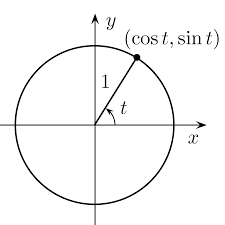
\includegraphics[scale=0.5]{UnitCircle.png}
\caption{The Unit Circle and Parametric Equations}
\label{unitcirc}
\end{center}
\end{figure}

Since these curves are defined as a function of a parameter, multiple different equations can describe the same curve. For example, $x=cos(2t)$ and $y=sin(2t)$. Because the range of the $sin$ and $cos$ functions are the same, these equations would draw out the same curve as Figure \ref{unitcirc}.

A \textbf{family} of parametric equations is a group of equations with the same parameter that trace out similar curves, normally by changing a constant. Circles, Lines, and Cycloids can be traced out using families of parametric equations.

\subsection{Calculus with Parametric Curves}
\subsubsection{Slope of a Parametric Curve}
By eliminating the parameter $t$ the parametric equations $x=f(t)$ and $y=g(t)$ can be written in the general form $h(x)$:
\begin{gather*}
    y = g(t) = h(f(t))
\end{gather*}
Applying the chain rule,
\begin{gather*}
y'(t) = g'(t) = h'(f(t))*f'(t) = h'(x)*f'(t)
\end{gather*}
If $f'(t) \neq 0$ then
\begin{gather*}
    h'(x) = \frac{g'(t)}{f'(t)}
\end{gather*}
This can be rewritten as:
\begin{gather*}
    \frac{d}{dx} (y) = \frac{dy}{dx} = \frac{\frac{dy}{dt}}{\frac{dx}{dt}}
\end{gather*}
By replacing $y$ with $\frac{dy}{dx}$:
\begin{gather*}
    \frac{d}{dx} (\frac{dy}{dx}) = \frac{d^2y}{dx^2} = \frac{\frac{d}{dt} (\frac{dy}{dx})}{\frac{dx}{dt}}
\end{gather*}
\subsubsection{Areas and Volumes with Parametrics}
Since the area under a curve of $y = h(x)$ is given by $\int_a^b h(x) dx$, a similar formula can be obtained for parametric equations where $x=f(t)$ and $y=g(t)$:
\begin{gather*}
    Area = \int_a^b y\hspace{2pt}dx = \int_c^d y \hspace{2pt} \frac{dx}{dt} \hspace{2pt}dt = \int_c^d g(t) * f'(t) \hspace{2pt} dt
\end{gather*}
Where $c$ is the left endpoint and $d$ is the right endpoint.
\linebreak\linebreak
A similar formula can be proved for the arc length of a parametric curve:
\begin{gather*}
    Arc\hspace{2pt}Length = \int_a^b \sqrt{1+(\frac{dy}{dx})^2} \hspace{3pt}dx
    = \int_c^d \sqrt{1+(\frac{\frac{dy}{dt}}{\frac{dx}{dt}})^2} \hspace{3pt} \frac{dx}{dt} \hspace{2pt} dt
    \linebreak\linebreak
    = \int_c^d \sqrt{(\frac{dx}{dt})^2 + (\frac{dy}{dt})^2} \hspace{3pt} dt
\end{gather*}
Even if the parametric curve cannot be expressed in the form $y=h(x)$ a limit Riemann sum can be used to prove this equation true.

The Surface Area of a solid of revolution can be derived similarly, using the non-parametric formula.

\begin{gather*}
    SA = \int_c^d 2\pi y \sqrt{(\frac{dx}{dt})^2 + (\frac{dy}{dt})^2} \hspace{3pt} dt
\end{gather*}
\subsection{Polar Coordinates}
\subsubsection{Defining Polar Coordinates}
Sometimes Cartesian coordinates are not convenient to represent some functions, where \textbf{polar coordinates} could be used. A \textbf{polar axis}, corresponding to the x-axis in Cartesian, is used as the base axis. Every point $P$ in the plane can be represented with two coordinates $(r,\theta)$, where $r$ is the distance from the origin to $P$ and $\theta$ is the angle between the polar axis and the line drawn from the origin to $P$, as seen in Figure \ref{polar}.

A point $(-r,\theta)$ can be defined as $(r,\theta+\pi)$. Because points are specified using angles around the polar axis, multiple coordinates can specify the same location. For example, the coordinates $(r,\theta)$ can also be written as:
\begin{gather*}
(r, \theta+2\pi n)
\end{gather*}
\begin{center}
    or
\end{center}
\begin{gather*}
(-r, \theta+(2n+1)\pi)
\end{gather*}
\begin{figure}[H]
\begin{center}
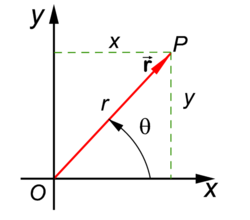
\includegraphics[scale=5]{MC11-polar.png}
\caption{Polar Coordinates}
\label{polar}
\end{center}
\end{figure}
Converting from polar to Cartesian coordinates can be done using trigonometric functions of $\theta$.
\begin{gather*}
    x = r cos(\theta)\hspace{50pt} y = r sin(\theta)
\end{gather*}
To convert from Cartesian to polar use:
\begin{gather*}
    r^2 = x^2 + y^2 \hspace{50pt} tan\hspace{2pt}\theta = \frac{y}{x}
\end{gather*}
The graph of a polar equation involves all points that can be represented using $(r,\theta)$ and whose coordinates make the equation true.\\
\subsubsection{Symmetry}
Polar symmetry can be used to help graph polar equations easier. Similar to Cartesian symmetry in $x$ and $y$, there are a few rules for polar symmetry.\\

If the Polar equation is unchanged when:
\begin{enumerate}
    \item $\theta$ is switched with $-\theta$, then the graph is symmetric over the polar axis.
    \item $r$ is switched with $-r$ or $\theta$ is replaced with $\theta + \pi$, the curve is symmetric about the origin(180 degree rotation symmetry).
    \item $\theta$ is replaced by $\pi - \theta$, then the graph is symmetric about the '$y$' axis, (the line $\theta = \frac{\pi}{2}$).
\end{enumerate}
\subsubsection{Slope of a Polar Curve}
To find the instantaneous slope or tangent line at a point on a polar curve, rewrite the polar function $r=f(\theta)$ as parametric equations with $\theta$ as a parameter.
\begin{gather*}
    x = r cos(\theta) = f(\theta)cos(\theta)\hspace{20pt}y = r sin(\theta) = f(\theta)sin(\theta)
\end{gather*}
Now by finding the slope of the now-parametric curve:
\begin{gather*}
    \frac{dy}{dx} = \frac{\frac{dy}{d\theta}}{\frac{dx}{d\theta}}
    = \frac{\frac{dr}{d\theta}*sin(\theta) + r cos(\theta)}{\frac{dr}{d\theta}*cos(\theta) - rsin(\theta)}
\end{gather*}
For the special case $r=0$:
\begin{gather*}
    \frac{dy}{dx} = tan(\theta) \hspace{5pt} for \hspace{5pt} \frac{dr}{d\theta} \neq 0
\end{gather*}
\subsection{Areas and Lengths in Polar Coordinates}
\subsubsection{Areas in Polar}
The area of a region bounded by a polar equation can be derived from the area of a sector of a circle(since polar equations also depend on the angle):
\begin{gather*}
    A = \frac{1}{2}r^2\theta
\end{gather*}
Where $A$ is the area and $\theta$ is measured in radians.

Given a region bounded by a curve $r=f(\theta)$ and the lines given by the polar equations $\theta=c$ and $\theta=d$, $0 < d - c \leqslant 2\pi$. Dividing the region into areas with equal width $\Delta \theta$, the area of Region $i$ can be approximated as:
\begin{gather*}
    A_i \approx \frac{1}{2} [f(\theta_i)]^2 * \Delta \theta
\end{gather*}
And so, a Riemann sum can be used to improve the approximation as $\Delta \theta \to 0$ and $n \to \infty$.
\begin{gather*}
    A = \lim_{n \to \infty} \sum_{i=1}^{n} \frac{1}{2} [f(\theta_i)]^2 * \Delta \theta = \int_c^d \frac{1}{2} [f(\theta_i)]^2 \hspace{2pt}d\theta
\end{gather*}
Since $r=f(\theta)$, this can also be written in a form similar to the circle sector formula:
\begin{gather*}
    A = \int_c^d \frac{1}{2} r^2 \hspace{2pt}d\theta
\end{gather*}
The area between two polar curves $f(\theta)$ and $g(\theta)$ can be derived using integral rules, where $j$ and $k$ are the angle coordinate of the points of intersection on both curves:
\begin{gather*}
    A = \frac{1}{2} \int_j^k ([f(\theta)]^2 - [g(\theta)]^2) \hspace{2pt}d\theta
\end{gather*}
The above works for $f(\theta) \geqslant g(\theta) \geqslant 0$ for all $\theta$ between $j$ and $k$.
\subsubsection{Lengths in Polar}
The Arc Length of a polar curve $r=f(\theta)$ between $\theta = a$ and $\theta = b$ can be found by treating $\theta$ as a parameter. This means that the parametric equations describing these are:

\begin{gather*}
    x = r * cos(\theta) = f(\theta)*cos(\theta)
\\
    y = r * sin(\theta) = f(\theta) * sin(\theta)
\end{gather*}
Using the product rule, where $r' = \frac{dr}{d\theta}$:
\begin{gather*}
    \frac{dx}{d\theta} = r' * cos(\theta) - r * sin(\theta)
    \\
    \frac{dy}{d\theta} = r' * sin(\theta) + r * sin(\theta)
\end{gather*}
Squaring both and adding yields:
\begin{gather*}
    (\frac{dx}{d\theta})^2 + (\frac{dy}{d\theta})^2 = (r')^2(sin^2(\theta) + cos^2(\theta)) + r^2(sin^2(\theta) + cos^2(\theta)) = r^2 + (\frac{dr}{d\theta})^2
\end{gather*}
Using the arc length formula(see 11.2), with $\theta$ as a parameter:
\begin{gather*}
    Arc\hspace{2pt}Length = \int_a^b \sqrt{r^2 + (\frac{dr}{d\theta})^2} \hspace{2pt} d\theta
\end{gather*}
\subsection{Conic Sections}
Parabolas, ellipses, and hyperbolas can be formed by the intersection of a plane with a cone, which is why they are often called \textbf{conics} or \textbf{conic sections}.
\subsubsection{Parabolas}
A \textbf{parabola} is formed when a plane cuts into a cone at an angle so that it intersects the cone's base. It is the set of points that are equidistant from a \textbf{focus} point $F$ and a line(called the \textbf{directrix}.) The point directly halfway between the directrix and focus lies on the parabola, and this is the \textbf{vertex}. The perpendicular through $F$ and intersecting the directrix is the parabola's \textbf{axis}.

If the focus is on the origin, then the focus of a basic parabola can be defined as the point $(0,p)$ and the directrix $y=-p$.

Using the distance formula, the distance between any point $P(x,y)$ on the parabola to the focus is:
\begin{gather*}
    |PF| = \sqrt{x^2 + (y-p)^2}
\end{gather*}
Similarly, the distance from the line to $P$(perpendicularly) is:
\begin{gather*}
    d(P,directrix) = |y+p|
\end{gather*}
By definiton, these two should be equal.
\begin{gather*}
    \sqrt{x^2 + (y-p)^2} = |y+p|\\
    x^2 + (y-p)^2 = (y+p)^2\\
    x^2 + y^2 -2py + p^2 = y^2 + 2py + p^2\\
    x^2 = 4py
\end{gather*}
If $a = \frac{1}{4p}$, then the standard form of a parabola based on the origin is:
\begin{gather*}
    y = \frac{x^2}{4p}\\
    y = ax^2
\end{gather*}
If $p > 0$ then the parabola opens up, and the opposite when $p < 0$. Replacing $y$ and $x$ reflects the parabola over the line $y=x$:
\begin{gather*}
    y^2 = 4px
\end{gather*}
\subsubsection{Ellipses}
An \textbf{ellipse} is formed when a plane intersects a cone and comes out on the other side without touching the base. It is the set of all points in a plane such that the sum of the distances from two focal points(\textbf{foci}) is constant.

Assuming the simplest case, where the foci are located on the x-axis at equal distances from the origin, the foci are located at points $(c,0)$ and $(-c,0)$. The constant distance sum is $2a$, greater than zero.

$P(x,y)$  is a point on the ellipse if
\begin{gather*}
    |PF_1| + |PF_2| = 2a\\
    \sqrt{(x+c)^2 + y^2} + \sqrt{(x-c)^2 + y^2} = 2a\\
    \sqrt{(x-c)^2 + y^2} = 2a - \sqrt{(x+c)^2 + y^2}\\
    x^2 - 2xc + c^2 + y^2 = 4a^2 - 4a\sqrt{(x+c)^2 + y^2} + x^2 + 2xc + c^2 + y^2\\
    a\sqrt{(x+c)^2+y^2} = a^2 + cx\\
    a^2(x^2 + 2xc + c^2 + y^2) = a^4 + 2a^2xc + x^2c^2\\
    (a^2 - c^2)x^2 + a^2y^2 = a^2(a^2-c^2)
\end{gather*}
Since $2c < 2a$(Triangle Inequality Theorem), we can define $b^2 = a^2 - c^2 > 0$. This becomes:
\begin{gather*}
    b^2x^2 + a^2y^2 = a^2b^2\\
    \frac{x^2}{a^2} + \frac{y^2}{b^2} = 1
\end{gather*}
When $y = 0$, the x-intercepts of the ellipse are $x = \pm a$. These points $(\pm a,0)$ are the the \textbf{vertices} of the ellipse and lie on its \textbf{major axis}. The y-intercepts are found to be $y = \pm b$. Since $x$ and $y$ are both squared in the equation, the ellipse is symmetric around both axes. A circle is just an ellipse where both foci are at the same point($c = 0$), and $r = a = b$.
\subsubsection{Hyperbolas}
A \textbf{hyperbola} made up of two branches can be formed by cutting two bases of a conic cone with a plane inclined vertically. It is the set of all points in a plane where the differences of distances from two \textbf{foci} are constant. Similar to an ellipse, where the distances from the points are added.

This means that for any point $P(x,y)$ on the hyperbola, $|PF_1| - |PF_2| = \pm 2a$, where $a$ is a constant. Using a similar method to an ellipse, the equation for any hyperbola is:
\begin{gather*}
    \frac{x^2}{a^2} - \frac{y^2}{b^2} = 1
\end{gather*}
Where the foci are at $x = \pm c$ so that $c^2 = a^2 + b^2$, with vertices at $x = \pm a$. The slant asymptotes are at $y = \pm (\frac{b}{a})x$. If the ellipse's major axis is on or parallel to the y-axis:
\begin{gather*}
    \frac{y^2}{a^2} - \frac{x^2}{b^2} = 1
\end{gather*}
Where the foci are at $y = \pm c$ so that $c^2 = a^2 + b^2$, with vertices at $y = \pm a$. The slant asymptotes are at $y = \pm (\frac{a}{b})x$.
\subsubsection{Shifting Conics}
The above equations were derived for a conic with major axis on the x-axis. These conics can be shifted by replacing $x$ and $y$ with $(x-h)$ and $(y-k)$ where $h$ and $k$ are the horizontal and vertical shifts.
\subsection{Conics in Polar Coordinates}
Instead of defining the ellipse and hyperbola with just foci, a more uniform definition can be applied to all conics:

Let point $F$ be a focus and $l$ be a directrix. $e$ is a constant, the \textbf{eccentricity}. A conic can be defined as the set of all points $P$ in a plane where
\begin{gather*}
    \frac{|PF|}{|Pl|} = e
\end{gather*}
This conic is an ellipse if $e < 1$, a parabola if $e = 1$, and a hyperbola if $e > 1$.
\begin{proof}
If $e = 1$, then the above becomes the definition of a parabola.
\\By converting $P$ to polar coordinates$(r,\theta)$, and setting $F$ at the origin:
\begin{gather*}
    |PF| = r \hspace{5pt} |Pl| = d - x = d - r cos(\theta)
\end{gather*}
Since $|PF| = e|Pl|$,
\begin{gather*}
    r = e(d - r cos(\theta))
\end{gather*}
Squaring both sides, and using $r^2 = x^2 + y^2$:
\begin{gather*}
    (1-e^2)x^2 + 2de^2x + y^2 = e^2d^2\\
    (x+\frac{e^2d}{1-e^2})^2 + \frac{y^2}{1-e^2} = \frac{e^2d^2}{(1-e^2)^2}
\end{gather*}
By completing the square above, that resembles the equation of an ellipse for $e < 1$ since $1-e^2 \geqslant 0$.
\begin{gather*}
    \frac{(x-h)^2}{a^2} + \frac{y^2}{b^2} = 1\\
    h = \frac{-e^2d}{1-e^2}\hspace{25pt}a^2 = \frac{e^2d^2}{(1-e^2)^2}\hspace{25pt}b^2 = \frac{e^2d^2}{1-e^2}
\end{gather*}
Finding the foci of this ellipse comes down to this,
\begin{gather*}
    c^2 = a^2 - b^2 = \frac{e^4d^2}{(1-e^2)^2}\\
    c = \frac{e^2d}{1-e^2} = -h
\end{gather*}
Remember the foci are at $(\pm c, 0)$. Now reducing two of the above equations yields,
\begin{gather*}
    e^2 = \frac{c^2}{a^2}\\
    e = \frac{c}{a}
\end{gather*}
If $e > 1$, that means that $1-e^2$ is now negative, which would only change the sign of $b^2$:
\begin{gather*}
    \frac{(x-h)^2}{a^2} - \frac{y^2}{b^2} = 1
\end{gather*}
This now fits the last case, the equation of the hyperbola.
\end{proof}
Since $r = e(d-rcos(\theta)$, the polar form of a conic is:
\begin{gather*}
    r = \frac{ed}{1 + cos(\theta)}
\end{gather*}
Now the directrix could be on the left too, in which case $x = -d$. Or it could be parallel to the y-axis where $y = \pm d$.
\begin{gather*}
    r = \frac{ed}{1 \pm e\hspace{2pt} cos(\theta)} \hspace{5pt}or \hspace{5pt}r = \frac{ed}{1 \pm e\hspace{2pt} sin(\theta)}
\end{gather*}
Which is an ellipse if $e < 1$, a parabola if $e = 1$, or a hyperbola if $e > 1$.
\section{Infinite Sequences and Series}
\subsection{Sequences}
\subsubsection{Defining Sequences}
A \textbf{sequence} is similar to a list of numbers that have an order:
\begin{gather*}
    a_1,a_2,a_3,a_4,...a_n
\end{gather*}
Where $a_1$ is the \textit{first term}, and $a_2$ is the \textit{second term}, so $a_n$ is the \textit{nth term}.

With infinite sequences, the sequence never ends, so every term $a_n$ has a term after it $a_{n+1}$.

Function properties can also be used by defining a function $f(n) = a_n$ where the domain is the positive integers.

A sequence can be defined explicitly($a_n=2n$) or implicitly($a_n = 5 + a_{n-1}$).
\subsubsection{Limits of Sequences}
Some sequences, such as $a_n = \frac{n}{n+1}$, can converge upon a certain value. This is seen by graphing $f(n) = \frac{n}{n+1}$. $a_n$ seems to be approaching 1 as $n$ increases unbounded.
\begin{gather*}
    1 - \frac{n}{n+1} = \frac{n-n+1}{n+1} = \frac{1}{n+1}
\end{gather*}
So by increasing $n \to \infty$:
\begin{gather*}
    \lim_{n\to \infty} \frac{1}{n+1} = 0
\end{gather*}
This means that
\begin{gather*}
    \lim_{n\to \infty} \frac{n}{n+1} = 1
\end{gather*}
Any sequence $\{a_n\}$ with a limit $L$ can be written as
\begin{gather*}
    \lim_{n\to \infty} a_n = L
\end{gather*}
This is true if $a_n$ can get arbitrarily close to $L$ by choosing some applicable(usually large) value of $n$. If $\lim_{n\to \infty} a_n$ exists, then $a_n$ \textbf{converges}. If not, then it \textbf{diverges}.

A more formal $\mathcal{E}$ definition of a sequence limit can also be used:

If a sequence $a_n$ has a limit $L$ if for every positive $\mathcal{E}$, there is some integer $N$ in the domain of $a_n$ where
\begin{gather*}
    |a_n - L| < \mathcal{E}\hspace{5pt}when\hspace{5pt}n > N
\end{gather*}
This works as $\mathcal{E}$ can be arbitrarily small.
To use function properties with sequences, a function $f(x)$ can be defined so that $f(n) = a_n$ for all $n$ in the domain of $a_n$. It follows that:

If $lim_{x \to \infty} f(x) = L$ and $f(n) = a_n$ for all $n$ in the domain of $a_n$, then $lim_{n \to \infty} a_n = L$.

However, since $a_n$ is only defined for positive integer $n$, a new definition of limits to infinity is needed:

    $\lim_{n \to \infty} a_n = \infty$ means that for every positive number $M$, there is an integer $N$ where  $a_n > M$ and $n > N$

Limit Laws work with series similar to how they work with functions.

The squeeze theorem can also apply:

If $a_n \leqslant b_n \leqslant c_n$ for all $n > n_0$ and $\lim_{n \to \infty} a_n = \lim_{n \to \infty} c_n = L$, then $\lim_{n \to \infty} b_n = L$
\subsubsection{Absolute and Conditional Convergence(Sequences)}
Absolute Convergence is when the sequence $|a_n|$ converges, as opposed to conditional convergence, when just $a_n$ does.
\begin{gather*}
    \textrm{If} \lim_{n \to \infty} |a_n| = 0, \textrm{then} \lim_{n \to \infty} a_n = 0
\end{gather*}
\begin{proof}
\begin{gather*}
    \textrm{Given:} \lim_{n \to \infty} |a_n| = 0\\
    1) -|a_n| \leqslant a_n \leqslant |a_n|\\
    2) \lim_{n \to \infty} -|a_n| = -\lim_{n \to \infty} |a_n| = 0\\
    3) \textrm{ By the squeeze theorem, } \lim_{n \to \infty} a_n = 0
\end{gather*}
\end{proof}
\subsubsection{Increasing, Decreasing, and Monotonic Sequences}
A sequence is \textbf{increasing} if $a_n < a_{n+1}$ for all $n \geqslant 1$, and \textbf{decreasing} if $a_n > a_{n+1}$ for the same condition. It is \textbf{monotonic} if the sequence is either always increasing or always decreasing.

A sequence is \textbf{bounded above} if there is some number $M$ where
\begin{gather*}
    a_n \leqslant M\textrm{ for all $n \geqslant 1$}
\end{gather*}
and \textbf{bounded below} if there is a number $N$ where
\begin{gather*}
    a_n \geqslant N\textrm{ for all $n \geqslant 1$}
\end{gather*}
If $a_n$ is bounded both above and below, then it is a \textbf{bounded} sequence.

\textbf{If a sequence is bounded and monotonic, then it is convergent}.
\begin{proof}
Given $a_n$, an increasing monotonic sequence, the set given by $S = \{a_n|n \geqslant 1\}$ has a least upper bound by the \textbf{Completeness Axiom} $L$. If $\mathcal{E} > 0$, then $L - \mathcal{E}$ is not an upper bound, since $L$ is the \textit{least} upper bound.
\begin{gather*}
    a_N > L - \mathcal{E}\textrm{ for some constant integer N}
\end{gather*}
Since the sequence is increasing, $a_n \geqslant a_N$ if $n > N$, so
\begin{gather*}
    a_n > L - \mathcal{E}\\
    0 \leqslant L - a_n < \mathcal{E}
\end{gather*}
The zero part is true since $a_n \leqslant L$. So:
\begin{gather*}
    |L - a_n| < \mathcal{E}
\end{gather*}
This is the $\mathcal{E}$ definition of a limit, so $\lim_{n \to \infty} a_n = L$, which proves convergence. A similar proof works if $a_n$ is decreasing.
\end{proof}
\subsection{Infinite Series}
\subsubsection{Series Convergence and Divergence}
By adding the terms of any infinite sequence, we get an \textbf{infinite series}, which is noted as:
\begin{gather*}
    \sum_{n=1}^{\infty} a_n
\end{gather*}
Though a lot of sums increase unbounded as $n \to \infty$, some \textbf{converge} upon a value, and cannot increase past it. For example, the series $\sum_{n=1}^{\infty} \frac{1}{2^n}$ will never increase past $1$, since every term after $n=2$ combined will never add up to $a_1 = \frac{1}{2}$. These convergences can be considered by looking at partial sums.

A \textbf{partial sum} is a finite sum of a number of terms of an infinite sequence:
\begin{gather*}
    S_n = a_1 + a_2 + a_3 ... a_n = \sum_{i=1}^n a_i
\end{gather*}
If $\lim_{n \to \infty} S_n = q$ is a real number $q$, then $\sum_{n=1}^\infty a_n$ is convergent with $\sum_{n=1}^\infty a_n = q$. The \textbf{sum} of the series is $q$, and if $q$ doesn't exist, then the infinite sum of $a_n$ diverges.
\subsubsection{Geometric Series}
A geometric series is any series of the form:
\begin{gather*}
    a + ar + ar^2 + ar^3 ... ar^{n-1} = \sum_{n=1}^\infty ar^{n-1}\hspace{7pt}a,r \neq 0
\end{gather*}
For the special case $r = 1$, $S_n = a + a + a... = na \to \pm \infty$, so this series diverges. However, if $-1 \leqslant r < 1$, then:
\begin{gather*}
    \textrm{The geometric series converges to} \sum_{n=1}^\infty ar^{n-1} = \frac{a}{1-r}
\end{gather*}
If $r$ has any other value, then this series diverges.
\begin{proof}
If $r \neq 1$:
\begin{gather*}
    S_n = a + ar + ar^2...ar^{n-1}\\
    r * S_n = ar + ar^2 + ar^3...ar^n\\
    S_n - r*S_n = a - ar^n = a(1 - r^n) = S_n(1-r)\\
    S_n = \frac{a(1-r^n)}{1-r} = \frac{a}{1-r} - \frac{ar^n}{1-r}
\end{gather*}
The sum of any series is $\lim_{q \to \infty} \sum_{n=1}^q a_n$:
\begin{gather*}
    \lim_{n \to \infty} S_n = \lim_{n \to \infty} [\frac{a}{1-r} - \frac{ar^n}{1-r}] = \frac{a}{1-r} - \frac{a}{1-r} * \lim_{n \to \infty} r^n
\end{gather*}
Since $\lim_{n \to \infty} r^n = 0 \textrm{ when } -1 < r < 1$:
\begin{gather*}
    \lim_{n \to \infty} S_n = \sum_{n=1}^\infty ar^{n-1} = \frac{a}{1-r}
\end{gather*}
\end{proof}
\subsubsection{Limits and the Divergence Test}
The limit of a sequence $a_n$ is strongly related to the convergence of its infinite series. In fact:
\begin{gather*}
    \textrm{If a series} \sum_{n = 1}^\infty a_n \textrm{ is convergent,}\lim_{n \to \infty} = 0
\end{gather*}
\begin{proof}
If $S_n$ is the partial sum of $a_n$ for all $n$ required, then any $a_n = S_n - S_{n-1}$. Since the series $a_n$ is convergent, its partial sum sequence $S_n$ is convergent. Let $\lim_{n \to \infty} S_n = q$, then since $n-1 \to \infty$ when $n \to \infty$, $\lim_{n \to \infty} S_n= lim_{n \to \infty} S_{n-1}= q.$
\begin{gather*}
    a_n = S_n - S_{n-1}\\
    \lim_{n \to \infty} a_n = \lim_{n \to \infty} S_n - \lim_{n \to \infty} S_{n-1} = q - q = 0
\end{gather*}
\end{proof}
However, the reverse of this is not necessarily true. For example, even though $\lim_{n \to \infty} \frac{1}{n} = 0$, the harmonic series diverges.

If a series is not convergent, it must be divergent. Since the limit of the terms of a convergent series must be 0, those that do not are divergent. This is the Divergence Test or the $n^{th}$ term test.
\begin{gather*}
    \textrm{If}\lim_{n \to \infty} a_n \neq 0 \textrm{ or DNE, then the series } \sum_{n = 1}^\infty a_n \textrm{ diverges.}
\end{gather*}
\subsubsection{Rules of Series}
Since all infinite sums can be rewritten as limits of partial sums, all the limit rules apply when using operations on infinite series. If $\sum a_n$ and $\sum b_n$are convergent, then
\begin{gather}
    \sum_{n = 1}^\infty c * a_n = c\sum_{n = 1}^\infty a_n\\
    \sum_{n = 1}^\infty(a_n + b_n) = \sum_{n = 1}^\infty a_n + \sum_{n = 1}^\infty b_n\\
    \sum_{n = 1}^\infty(a_n - b_n) = \sum_{n = 1}^\infty a_n - \sum_{n = 1}^\infty b_n
\end{gather}
All of the above series are convergent. In (1), $c$ is a constant. This shows the sum or difference of two convergent series are also convergent.
\subsection{The Integral Test and Estimates of Sums}
\subsubsection{Improper Integrals and Infinite Series}
Sometimes it is really difficult to get the sum of an infinite series, and so it is often more useful to find if the series converges/diverges.

This can be done by drawing the graph of $f(n) = a_n$ and drawing Riemann approximations of width 1, since that means the area of each box would be $f(n) * 1 = a_n$. Now assume as $n \to \infty$, $f(n)$ eventually becomes decreasing and positive.

Now, by using the value of the infinite(improper) integral, it is possible to use an upper or lower bound on $\sum a_n$. For example, to prove convergence:
\begin{gather*}
    \sum_{n = 1}^\infty a_n < \int_1^\infty f(x)\hspace{3pt}dx = c
\end{gather*}
This means that the series of $a_n$ must be less than $c$, a finite constant. This means that $a_n$ must converge.

Similarly, if the integral diverged, and $\sum a_n > \int f(x) dx$, then the series would have to be infinite and diverge. This leads to the integral test:

If $f(x)$ is a continuous function on $[1,\infty]$ and positive and decreasing as $n \to \infty$ where $f(n) = a_n$, then:
\begin{gather}
    \textrm{If } \int_1^\infty f(x)\hspace{3pt}dx\textrm{ converges, then }\sum_{n=1}^\infty a_n \textrm{ converges.}\\
    \textrm{If } \int_1^\infty f(x)\hspace{3pt}dx\textrm{ diverges, then }\sum_{n=1}^\infty a_n \textrm{ diverges.}
\end{gather}
If the series starts at $n=c$, the integral $\int_c^\infty f(x)\hspace{3pt}dx$ should be used.
\subsubsection{The p-series test}
The integral test can also be used to prove the p-series test below:
\begin{gather*}
    \textrm{The series} \sum_{n=1}^\infty \frac{1}{n^p} \textrm{ converges only if } p > 1
\end{gather*}
\subsubsection{Estimating the Sum of a Series}
Now if $\sum a_n$ is convergent, then it has a sum $s$. While the integral test cannot be used to find the sum of a series, it is possible to find an approximation. Any partial sum $S_n$ is an approximation that gets better as $n \to \infty$, since $\lim_{n \to \infty} S_n = s$. The \textbf{remainder} is the error in the approximation, simply:
\begin{gather*}
    R_n = s - S_n = a_{n+1} + a_{n+2} + a_{n+3}...
\end{gather*}
Using the Riemann sum approximation from the previous section, the partial sum $S_n$ represents all the boxes from $a_1$ to $a_n$ so $R_n$ represents the boxes that are remaining(hence $s - S_n$). So if $f(x)$ is decreasing
\begin{gather*}
    R_n \leqslant \int_n^\infty f(x)\hspace{3pt}dx
\end{gather*}
Modifying the Reimann approximation a little, using the left side instead of the right, a new picture can be drawn, where the $a_{n+1}$ box is above the curve, as well as all the boxes after. This can be done by translating to the right 1 unit(see Figure 3/4 in 12.2). Since the approximation is above the curve:
\begin{gather*}
    R_n \geqslant \int_{n+1}^\infty f(x)\hspace{3pt}dx
\end{gather*}
This leads to: Given $f(m) = a_m$, and f is continuous, positive, and decreasing over $[n,\infty]$. If $\sum a_n$ converges,
\begin{gather*}
     \int_{n+1}^\infty f(x)\hspace{3pt}dx \leqslant R_n \leqslant \int_n^\infty f(x)\hspace{3pt}dx
\end{gather*}
By adding $S_n$ to both sides, since $s = R_n + s$:
\begin{gather*}
    S_n + \int_{n+1}^\infty f(x)\hspace{3pt}dx \leqslant s \leqslant S_n + \int_n^\infty f(x)\hspace{3pt}dx
\end{gather*}
\subsubsection{Formal Proof of the Integral Test}
\begin{proof}
Using the Reimann approximation where the rectangles are under the curve(starting at $n+1 = 1+1 = 2$):
\begin{gather*}
    a_2 + a_3 + a_4....a_n \leqslant \int_1^n f(x)\hspace{3pt}dx
\end{gather*}
Shifting to the left one unit:
\begin{gather*}
    \int_1^n f(x)\hspace{3pt}dx \leqslant a_1 + a_2 + a_3...a_{n-1}
\end{gather*}
Since $f(x) > 0$:
\begin{gather*}
    \sum_{i = 2}^n a_i \leqslant \int_1^n f(x)\hspace{3pt}dx \leqslant \int_1^\infty f(x)\hspace{3pt}dx
\end{gather*}
If $\int f(x)\hspace{3pt}dx$ converges to M, and $S_n = a_1 + \sum_{i = 2}^n a_i$:
\begin{gather*}
    S_n = a_1 + \sum_{i = 2}^n a_i \leqslant a_1 + \int_1^\infty f(x)\hspace{3pt}dx = M\\
    S_n \leqslant M
\end{gather*}
Since $a_n > 0$, $S_{n+1} > S_n$, and so $S_n$ is an increasing and monotonic sequence, which means $S_n$ is a convergent sequence, which means $\sum a_n$ is also convergent.

If $\int_1^\infty f(x)\hspace{3pt}dx$ diverges then $\int_1^n f(x)\hspace{3pt}dx \to \infty \textrm{ as } n \to \infty$. From the second Riemann sum:
\begin{gather*}
    \int_1^n f(x)\hspace{3pt}dx \leqslant \sum_{i=1}^{n-1} a_i = S_{n-1}
\end{gather*}
This shows that $S_{n-1} \to \infty$, which means $S_n \to \infty$ and $\sum a_n$ diverges.
\end{proof}
\subsection{The Comparison Tests}
Sometimes a smart way to check for convergence is by comparing to an easier series. For example, if $a_n < b_n$ and $b_n$ is convergent, then $a_n$ also has to be convergent, given that $a_n$ is increasing as $n \to \infty$. This idea only works when both series are positive(since \textit{series} are increasing the \textit{sequences} must be positive). The opposite logic works when negative.
\subsubsection{The Direct Comparison Test}
Let $\sum a_n$ and $\sum b_n$ be series with positive terms:
\begin{gather}
    \textrm{If } \sum b_n \textrm{ converges and } a_n \leqslant b_n\textrm{(for all n $\to \infty$) then } \sum a_n \textrm{ converges.}\\
    \textrm{If } \sum b_n \textrm{ diverges and } a_n \geqslant b_n\textrm{(for all n $\to \infty$) then } \sum a_n \textrm{ diverges.}
\end{gather}
\begin{proof}
(1) Let $s_n$ and $t_n$ be the partial sums of $a_n$ and $b_n$, respectively. Since $b_n$ converges(see (1) above), it has an infinite sum $t$. Since both \textit{sequences} are positive, their \textit{series} must be increasing. Since $a_n \leqslant b_n$, $s_n \leqslant t_n \leqslant t$. Since $s_n \leqslant t$, the series $\sum a_n$ is now bounded above \textit{and} increasing, so it must be convergent.

(2) If $b_n$ diverges, that means that $t_n \to \infty$($b_n$ is increasing so it can't go to $-\infty$). Since $a_n \geqslant b_n, s_n \geqslant t_n$. $\therefore$ $ s_n \to \infty$ and $\sum a_n$ diverges.
\end{proof}
\subsubsection{The Limit Comparison Test}
However, when $a_n$ is greater than a convergent series or less than a divergent series, the Direct Comparison test is useless. However, another kind of comparison test can help.

Let $\sum a_n$ and $\sum b_n$ be series with positive terms. Given that:
\begin{gather*}
    \lim_{n \to \infty} \frac{a_n}{b_n} = c
\end{gather*}
Where $c$ is any constant where $c > 0$. This means that both series either converge or diverge. In other words, if one converges then the other one does too, same for divergence.
\begin{proof}
Let $m$ and $M$ be two different positive numbers where $m < c < M$. Since $\frac{a_n}{b_n} \to c$ as $n$ gets very large, there must be some large integer $N$ where when $n > N$:
\begin{gather*}
    m < \frac{a_n}{b_n} < M \implies mb_n < a_n < Mb_n
\end{gather*}
If $\sum b_n$ converges, so does $M \sum b_n$. $a_n < Mb_n \therefore a_n$ converges. Similar logic can be used for divergence with $a_n > mb_n$.
\end{proof}
\subsubsection{Estimating Sums: Comparison Tests}
Series comparisons can also be used to \textit{bound} the error on a series. For example, the remainder of a series $a_n$ is $R_n$:
\begin{gather*}
    R_{a_n} = s - S_n = a_{n+1} + a_{n+2} + a_{n+3}...\\
    R_{b_n} = t - T_n = b_{n+1} + b_{n+2} + b_{n+3}...
\end{gather*}
Now since $a_n \leqslant b_n$, $R_{a_n} \leqslant R_{b_n}$(see above for why). The Comparison Test can be used in combination with the integral test to bound the error of more series:
\begin{gather*}
    R_{a_n} \leqslant R_{b_n} \leqslant \int_n^\infty f(x)\hspace{2pt}dx
\end{gather*}
\subsection{Alternating Series}
Some series contain terms that are not always positive, and one very important one is the \textbf{alternating series}. An alternating series is one where the series changes sign every term, for example:
\begin{gather*}
    \sum_{n=1}^\infty \frac{(-1)^{n-1}}{n} = 1 - \frac{1}{2} + \frac{1}{3} - \frac{1}{4} + \frac{1}{5}...
\end{gather*}
\subsubsection{The Alternating Series Test}
If an alternating series $\sum a_n = \sum_{n=1}^\infty (-1)^{n-1}b_n$ satisfies the following:
\begin{gather}
    b_n > 0\\
    b_{n+1} \leqslant b_n \textrm{ for all n($b_n$ is decreasing or constant)}\\
    \lim_{n \to \infty} b_n = 0
\end{gather}
Then $\sum a_n$ is convergent.

Before the formal proof, consider the logical proof. If an alternating series converges, it will be oscillating around a convergence value. If the terms in $b_n$ are decreasing, then the amplitude of oscillation will decrease as the series closes in on its sum. However, if $b_n$ is increasing(or never reaches zero), the series will never close in and converge.
\begin{proof}
Since all the even partial sums are increasing and the odds are decreasing(remember the series alternates):
\begin{gather*}
    S_2 = a_1 - a_2 \geqslant 0 \textrm{ since $a_2 \leqslant a_1$}\\
    S_4 = s_2 + (a_3 - a_4) \geqslant S_2 \textrm{ since $a_4 \leqslant a_3$}\\
    \textrm{For all even partial sums($S_{2n}$):}\\
    S_{2n} = S_{2n-2} + (a_{2n-1} - a_{2n}) \geqslant S_{2n-2} \textrm{ since $a_{2n} \leqslant a_{2n-1}$}
\end{gather*}
This shows that all the even partial sums are positive and increasing. All the even partial sums can be written as:
\begin{gather*}
    S_{2n} = a_1 - (a_2 - a_3) - (a_4 - a_5) ... - (a_{2n-2} - b_{2n-1}) - b_{2n}
\end{gather*}
Looking back at the quantities in parentheses, they are all positive, so $S_{2n}$ will never exceed $a_1$. Since $S_{2n}$ is increasing and bounded by $a_1$ it must be convergent, with a sum of $s$. Now for the odd partial sums:
\begin{gather*}
    \lim_{n \to \infty} s_{2n+1} = \lim_{n \to \infty} s_{2n} + \lim_{n \to \infty} a_{2n+1}
\end{gather*}
The second limit is zero by (3) of the series test above.
\begin{gather*}
    = s + 0 = s
\end{gather*}
Since the even and odd partial sums approach the same value $s$, the alternating series converges.
\end{proof}
\subsubsection{Estimating Sums: Alternating Series}
Alternating Series can also be used to estimate and bound the error of a partial sum.

If $\sum a_n$ is an alternating series that converges by the alternating series test(satisfies all conditions), then:
\begin{gather*}
    |R_n| = |s - S_n| \leqslant a_{n+1}
\end{gather*}
\begin{proof}
The following can be seen from the Alternating Series Test(see figure from textbook, visual intuition)
\begin{gather*}
    |R_n| = |s - S_n| \leqslant |S_{n+1} - S_n| = a_{n+1}\\
    |R_n| \leqslant a_{n+1}
\end{gather*}
\end{proof}
\subsection{Absolute Convergence and the Ratio and Root Tests}
\subsubsection{Absolute Convergence}
Many of the convergence tests only work when the series is always positive or alternating, but what if it isn't? With any given series $\sum a_n$, another series $\sum |a_n|$ can be used(useful since all terms are now positive or zero).

A series is \textbf{absolutely convergent} if $\sum |a_n|$ converges. Of course, this fact is not useful with positive $a_n$, since $|a_n| = a_n$ in that case.

Sometimes, series can be convergent, but not absolutely convergent. Example would be $a_n = \frac{(-1)^{n-1}}{n}$. This series converges by the Alternating Series Test, but $|a_n| = \frac{1}{n}$ diverges(harmonic series). When this happens, $a_n$ is called \textbf{conditionally convergent}.

However, the usefulness here comes from the following fact:
\begin{gather*}
    \textrm{If } \sum |a_n| \textrm{ converges, then } \sum a_n \textrm{ converges.}
\end{gather*}
\begin{proof}
\begin{gather*}
    0 \leqslant a_n + |a_n| \leqslant 2|a_n|
\end{gather*}
$2|a_n|$ must converge since $|a_n|$ converges, and therefore $a_n + |a_n|$ converges due to the direct comparison test. Since $a_n = (a_n + |a_n|) - (|a_n|)$, and both series in parenthesis are convergent, $a_n$ must be convergent.
\end{proof}
\subsubsection{The Ratio Test}
This test is often a very useful one:
\begin{gather}
    \textrm{If} \lim_{n \to \infty} |\frac{a_{n+1}}{a_n}|= L < 1, \textrm{then } \sum a_n \textrm{ converges.}\\
    \textrm{If} \lim_{n \to \infty} |\frac{a_{n+1}}{a_n}|= L > 1, \textrm{then } \sum a_n \textrm{ diverges.}\\
    \textrm{If} \lim_{n \to \infty} |\frac{a_{n+1}}{a_n}|= L = 1, \textrm{then Ratio Test is inconclusive.}
\end{gather}
\begin{proof}
To prove case (1), compare the given series to a convergent geometric series($r < 1$). Since $L < 1$ there has to be an $L < r < 1$ that fits between $L$ and $1$.
\begin{gather*}
    \lim_{n \to \infty} |\frac{a_{n+1}}{a_n}|= L < r < 1
\end{gather*}
After some $n = N$, the ratio $|\frac{a_{n+1}}{a_n}|$ will eventually become less than $r$:
\begin{gather*}
    |\frac{a_{n+1}}{a_n}| < r \textrm{ for $n \geqslant N$}\\
    |a_{n+1}| < |a_n|r \textrm{ for all $n \geqslant N$}
\end{gather*}
By using $N,N+1,N+2...$ into the equation:
\begin{gather*}
    |a_{N+1}| < |a_N|r\\
    |a_{N+2}| < |a_{N+1}|r < |a_N|r^2\\
    |a_{N+3}| < |a_{N+2}|r^3\\
\end{gather*}
A more general form:
\begin{gather*}
    |a_{N+k}| < |a_N|r^k
\end{gather*}
Now consider a (separate) geometric series :
\begin{gather*}
    \sum_{k=1}^\infty |a_N|r^k = |a_N|r + |a_N|r^2 + |a_N|r^3...
\end{gather*}
This series is convergent because it's a geometric series with common ratio $r$, remember from before $r < 1$. Since $|a_{N+k}| < |a_N|r^k$, the direct comparison test shows that the former converges. Remember since a finite number of terms doesn't effect the final outcome, if $\sum a_{N+k}$ converges, so does $\sum a_n$.

If $L >1$, then that means that eventually there must be an integer $N$ where:
\begin{gather*}
    |\frac{a_{n+1}}{a_n}| > 1\textrm{ for $n \geqslant N$}\\
    |a_{n+1}| > |a_n|
\end{gather*}
Therefore $a_n$ is increasing and $\lim_{n \to \infty} \neq 0$. This means $a_n$ diverges by the $n^{th}$ term test.
\end{proof}
\subsubsection{The Root Test}
This one is very similar to the ratio test:
\begin{gather}
    \textrm{If} \lim_{n \to \infty} \sqrt[n]{|a_n|} = L < 1, \textrm{then $\sum a_n$ converges.}\\
    \textrm{If} \lim_{n \to \infty} \sqrt[n]{|a_n|} = L > 1, \textrm{then $\sum a_n$ diverges.}\\
    \textrm{If} \lim_{n \to \infty} \sqrt[n]{|a_n|} = L = 1, \textrm{then the root test is inconclusive.}
\end{gather}
Note: \textbf{If $L=1$ on the ratio test, do not try the Root Test.}
\begin{proof}
The proof here is very similar to the Ratio Test. Let $r$ be a number so that it fits inside $L < r < 1$. There must be some large integer $N$ so that after that $\sqrt[n]{|a_n|} < r$.
\begin{gather*}
    \sqrt[n]{|a_n|} < r\textrm{ for $n \geqslant$ N}\\
    |a_n| < r^n
\end{gather*}
Now create a geometric series like so:
\begin{gather*}
    \sum_{n = 1}^\infty r^n = r + r^2 + r^3... \implies \textrm{converges since $r < 1$.}\\
    \sum_{n = 1}^\infty |a_n| < \sum_{n = 1}^\infty r^n \implies \sum a_n \textrm{ converges by Direct Comparison/Abs. Conv.}
\end{gather*}
Similarly, if $L > r > 1$, then $|a_n| > r^n$, which now diverges. By the comparison test, $a_n$ now diverges.
\end{proof}
\subsubsection{Rearranging Series}
Unlike with finite addition, the commutative property does not apply to infinite sums, which means rearranging terms can actually change the value of the series. A \textbf{rearrangement} of a series means changing the order of the terms in the series.

If a series has absolute convergence, it means that any rearrangement of the terms will not change the final sum. \textbf{However, if a series is conditionally convergent, given any real number $m$ there is sum rearrangement of terms that will result in a final sum of $m$.}
\subsection{Testing Series}
Testing series convergence can be difficult, but can be expedited by recognizing which series fit which tests the best, especially according to their general form.
\begin{enumerate}
    \item Before doing anything, if $\lim_{n \to \infty} a_n \neq 0$, $a_n$ automatically diverges.
    \item If $a_n$ is in some form of $\frac{1}{n^p}$, then the p-series test is the easiest to use.
    \item If the series has a similar form to a geometric series, more specifically where multiplying $a_n$ by a number $r$ gives $a_{n+1}$, the geometric series test can be used($|r| < 1$).
    \item If the series is similar to any of the other tests(especially geometric or p-series), a Direct or Limit Comparison normally does the trick. For example, if $a_n$ is similar to a p-series(ex. a polynomial), only the highest power of the numerator and/or denominator should be used in the compared series, since then $a_n < \textrm{p-series.}$
    \item If the series has a $(-1)^{n-1}$ or $(-1)^n$, try alternating series.
    \item If the series has irregularly signed terms, try testing for convergence for $\sum |a_n|$.
    \item Factorials and exponentials are often good with the Ratio or Root tests. \textbf{The Ratio or Root Tests do not work with algebraic/polynomial expressions.}
    \item If $\int f(x) dx$ is easy to evaluate, the Integral Test is a good option(make sure it fits the test though).
\end{enumerate}
\subsection{Power Series}
A \textbf{power series} is any series of the form:
\
\begin{gather*}
    \sum_{n=0}^\infty c_n x^n = c_0 + c_1 x + c_2 x^2 + c_3 x^3...
\end{gather*}
All $c$ are constants. Notice that this series starts with $n = 0$ instead of the normal $n=1$, which means $x^0 = 1$ and the first term will always be a constant $c_0$.

An example would be the power series given by $c_n = 1$, which would yield $\sum x^n$, the classic geometric series. This series converges when $|r| < 1$, or in this case when $|x| < 1$.

Normally, power series are more general, in the way that they can be shifted:
\begin{gather*}
    \sum_{n = 0}^\infty c_n (x-a)^n = c_0 + c_1 (x-a) + c_2 (x-a)^2...
\end{gather*}
This is also a power series, but one that is \textbf{centered at a}. All power series are convergent at $a$, because when $x \to a$, every term except $c_0$ is zeroed out and the series converges to $c_0$.

With power series, since they are full of exponentials, the Ratio Test(and sometimes Root Test) are very useful to find convergence. However, since the Ratio Test fails at $1$, other tests must be used to find convergence and divergence when the ratio test yields 1.

For any power series $\sum_{n = 0}^\infty c_n (x-a)^n,$ one of the following must be true:
\begin{gather}
    \textrm{The series converges only when } x = a.\\
    \textrm{The series converges for all } x.\\
    \textrm{The series converges when $|x-a| < R$ and diverges when $|x-a| > R$.}
\end{gather}
(3) is true for a positive number $R$(could be $0$ or $\infty$). Basically, the inequalities in (3) suggest there is an \textbf{interval of convergence}, where $a - R < x < a + R$, and the series converges. In this case, $R$ is the \textbf{radius of convergence}. Of course, the endpoints of this interval could converge or diverge, and that must be tested separately.
\subsection{Functions as Power Series}
\subsubsection{Functions as Geometric Series}
Because the sum of a convergent geometric series is $\frac{a}{1-r}$, many functions can actually be represented as sums of infinite geometric series. This makes it easier to differentiate/integrate, and to approximate. For example
\begin{gather*}
    f(x) = \frac{1}{1-x} = \sum_{n=0}^\infty x^n = 1 + x + x^2 + x^3...
\end{gather*}
In this case $r=x$, and remember this only works when $|x| < 1$, because otherwise the series does not converge.
\subsubsection{Differentiating and Integrating Power Series}
Because series are just sums, integrating and differentiating are easier on them than on their functional equivalents. This means utilizing something called \textbf{term-by-term differentiation or integration}, which uses the fact that the derivative of a sum is equal to the sum of the derivatives of each term, and same for integration, as follows:

If a power series $\sum_{n=0}^\infty c_n (x-a)^n$ has a radius of convergence $R > 0$, then $f(x)$, the function defined by the series is differentiable(and continuous) on $(a-R, a+R)$, and:
\begin{gather*}
    f'(x) = c_1 + 2c_2(x-a) + 3c_3(x-a)^2... = \sum_{n=1}^\infty nc_n(x-a)^{n-1}\\
    \int f(x) dx = c_0(x-a) + c_1\frac{(x-a)^2}{2} + c_2\frac{(x-a)^3}{3}...+C = \sum_{n=0}^\infty c_n \frac{(x-a)^{n+1}}{n+1} + C
\end{gather*}
The above comes from these simple rules:
\begin{gather}
    \frac{d}{dx} \bigg[\sum_{n=0}^\infty c_n(x-a)^n\bigg] = \sum_{n=0}^\infty \frac{d}{dx} \big[c_n(x-a)^n\big]\\
    \int \bigg[\sum_{n=0}^\infty c_n(x-a)^n\bigg] dx= \sum_{n=0}^\infty \int \big[c_n(x-a)^n\big] dx
\end{gather}
\subsection{Taylor and Maclaurin Series}
In the last section, we could find power series for functions that fit the geometric series($f(x) = \frac{a}{1-r}$). But what about for other functions, like maybe $f(x) = sin(x)$? This can be done by looking at power series in more general terms:
\begin{gather*}
    f(x) = c_n (x-a)^n = c_0 + c_1 (x-a) + c_2 (x-a)^2...
\end{gather*}
The only thing that could possibly change are the coefficients $c_n$, so $c_0$ can be found by using $x = a$:
\begin{gather*}
    f(a) = c_0 + c_1(a-a) + c_2(a-a)... = c_0
\end{gather*}
\subsubsection{Taylor and Maclaurin Series}
Now taking the derivative eliminates $c_0$, and "shifts" the function down one coefficient:
\begin{gather*}
    f'(x) = c_1 + 2c_2(x-a) + 3c_3(x-a)^2...
\end{gather*}
The same idea here:
\begin{gather*}
    f'(a) = c_1
\end{gather*}
However, things get a little more complicated when you take the next few:
\begin{gather*}
    f''(a) = 2c_2\\
    f^3(a) = 6c_3 = 3! * c_3
\end{gather*}
And the pattern continues, because the power rule multiplies the current coefficient by $(n-1)$ when taking a derivative, which means the final coefficient is going to be $n(n-1)(n-2)... = n!$ This leads to:
\begin{gather*}
    f^n(a) = n! c_n\\
    c_n = \frac{f^{(n)}a}{n!}
\end{gather*}
This means that if $f(x)$ has a power series form at $x = a$:
\begin{gather*}
    \textrm{If } f(x) = \sum_{n=0}^\infty c_n(x-a)^n\textrm{ and }|x-a| < R\\
    \textrm{then }c_n = \frac{f^{(n)}(a)}{n!}
\end{gather*}
For the special case $a = 0$, the series is called the \textbf{Maclaurin Series}:
\begin{gather*}
    f(x) = \sum_{n=0}^\infty \frac{f^{(n)}(0)}{n!} = f(0) + \frac{f'(0)}{1}x + \frac{f''(0)}{2!}x^2...
\end{gather*}
However, this is only an approximation(which gets worse away from $a$ and with fewer terms). When is a a Taylor series equal to the function(inside the radius of convergence)?

If $f(x)$ is equal to its Taylor series, then that must meant that $f(x) = \lim_{n \to \infty} T_n$, where $T_n$ are \textbf{nth degree Taylor polynomials}:
\begin{gather*}
    T_n = \sum_{i = 0}^n \frac{f^{(i)}(a)}{i!}(x-a)^i = f(a) + \frac{f'(a)}{1!}(x-a) + \frac{f''(a)}{2!}(x-a)^2...\frac{f^{(n)}(a)}{n!}(x-a)^n
\end{gather*}
As $n$ gets larger $T_n$ is a better approximation of $f(x)$, especially around $a$. This makes sense because $n=1$ is only going to be linear, $n=2$ quadratic, and so on.

So as $n \to \infty, f(x)$ is the sum of its taylor series if:
\begin{gather*}
    f(x) = \lim_{n \to \infty} T_n(x)
\end{gather*}
Now for any $n$, the difference between $f(x)$ and $T_n(x)$ is the \textbf{remainder} $R_n(x)$:
\begin{gather*}
    R_n(x) = f(x) - T_n(x)\\
    f(x) = R_n(x) + T_n(x)
\end{gather*}
Now if we find $\lim_{n \to \infty} R_n(x) = 0$, then:
\begin{gather*}
    \lim_{n \to \infty} T_n(x) = \lim_{n \to \infty}\bigg[f(x) - R_n(x)\bigg] = f(x)
\end{gather*}
It follows that if $\lim_{n \to \infty} R_n(x) = 0$, then $f(x)$ is equal to the sum of its Taylor series on $|x-a| < R$.
\subsubsection{Taylor's Inequality}
If $|f^{(n+1)}| \leqslant M$ for $|x-a| \leqslant d$, then the remainder $R_n(x)$:
\begin{gather*}
    |R_n(x)| \leqslant \frac{M}{(n+1)!}|x-a|^{n+1}
\end{gather*}
\begin{proof}
Consider the case $n = 1$, assuming that $|f''(x)|\leqslant M \implies f''(x) \leqslant |f''(x)| \leqslant M$. For $a \leqslant x \leqslant a+d$(not $a-d$ because integral starts at $a$):
\begin{gather*}
    \int_a^x f''(t) dt \leqslant \int_a^x M dt\\
\end{gather*}
So using the FTC:
\begin{gather*}
    f'(x) - f'(a) \leqslant M(x-a)\\
    f'(x) \leqslant f'(a) + M(x-a)
\end{gather*}
Now repeating:
\begin{gather*}
    \int_a^x f'(t) dt \leqslant \int_a^x \big[f'(a) + M(t-a)\big] dt\\
    f(x) - f(a) \leqslant f'(a)(x-a) + M\frac{(x-a)^2}{2}\\
    f(x) - f(a) - f'(a)(x-a) \leqslant M\frac{(x-a)^2}{2}
\end{gather*}
Remember $R_1(x) = f(x) - T_1(x) = f(x) - f(a) - f'(a)(x-a)$:
\begin{gather*}
    R_1(x) \leqslant \frac{M}{2}(x-a)^2
\end{gather*}
Now since $|f''(x)| \leqslant M, f''(x) \geqslant -M$, which gives(using a similar process as above):
\begin{gather*}
    R_1(x) \geqslant -\frac{M}{2}(x-a)^2\\
    |R_1(x)| \leqslant \frac{M}{2}(x-a)^2\\
    |R_1(x)| \leqslant \frac{M}{2}|x-a|^2
\end{gather*}
The last step required that $x > a$, but this is true when $x < a$ also. This proves the case $n = 1$ by integrating 2 times. Each $n$ case can be proved by integrating $n + 1$ times, to match $T_n(x)$.
\end{proof}
Taylor series are important because now it is possible to integrate functions that did not have easy anti-derivatives. For example, $f(x) = e^{-x^2}$ was not possible to integrate because there was no $2x$, but using series it is now.
\subsubsection{Multiplying and Dividing Power Series}
We know that adding and subtracting series behaves like polynomials do. However, it is also possible to multiply and divide them(ex. $f(x) = tan(x) = \frac{sin(x)}{cos(x)}$.

In fact, multiplying and dividing can be done just as for normal polynomials(ex. foiling(not useful for infinite series though), vertical multiplication, and long division).
\subsection{The Binomial Series}
These series expansions can be extended to functions under the Binomial Theorem, which is:
\begin{gather*}
    (a+b)^k = a^k + ka^{k-1}b + \frac{k(k-1)}{2!}a^{k-2}b^2 + \frac{k(k-1)(k-2)}{3!}a^{k-3}b^3...\\
    \binom{k}{0} = 1\\ \binom{k}{n} = \frac{k(k-1)(k-2)...(k-n+1)}{n!} \textrm{ for $n = 1,2..k$}\\
    (a+b)^k = \sum_{n=0}^k \binom{k}{n}a^{k-n}b^n
\end{gather*}
If $a = 1$ and $b = x$, then:
\begin{gather*}
    (a+b)^k = (1+x)^k = f(x) = \sum_{n=0}^k \binom{k}{n}x^n
\end{gather*}
However, the Binomial Theorem only works when $k$ is a positive integer, so to extend this construct a Maclaurin series off of $f(x)$:
\begin{gather*}
    f(x) = (1+x)^k\hspace{20pt}f(0) = 1\\
    f'(x) = k(1+x)^{k-1}\hspace{20pt}f'(0) = k\\
    f''(x) = k(k-1)(1+x)^{k-2}\hspace{20pt}f''(0) = k(k-1)\\
    f^{(n)}(x) = k(k-1)...(k-n+1)(1+x)^{k-n}\hspace{20pt}f^{(n)}(0) = k(k-1)...(k-n+1)
\end{gather*}
Now the Maclaurin series can be constructed:
\begin{gather*}
    \sum_{n=0}^\infty \frac{f^{(n)}(0)}{n!}x^n = \sum_{n=0}^\infty \frac{k(k-1)...(k-n+1)}{n!}x^n = \sum_{n=0}^\infty \binom{k}{n}x^n
\end{gather*}
By the Ratio Test:
\begin{gather*}
    \lim_{n \to \infty}|\frac{a_{n+1}}{a_n}| = \lim_{n \to \infty} \frac{|k-n|}{n+1}|x| = |-1||x| = |x|
\end{gather*}
So, this series converges when $|x| < 1$ and diverges when $|x| > 1$. However, the convergence at the endpoints depends on $k$. The series converges at $x = 1$ when $-1 < k < 0$ and at $\pm 1$ when $k \geqslant 0$. Remember that $\binom{k}{n}$ builds and adds factors each time. If $k$ is a positive integer and $n > k$, then there will eventually be a $(k-k) = 0$ factor in the numerator and the rest of the series will zero out. This means the series is not infinite anymore and actually reduces down to the normal binomial theorem.
\section{Vectors and the Geometry of Space}
\subsection{3D Coordinate Systems}
On a plane, a specific point can be found using only two numbers, $a$ and $b$. The point $(a,b)$ specifies the distance in the $x$ and $y$ directions of the location of the point relative to some origin point. Similarly, in 3D space, three numbers $(a,b,c)$ are needed. Also, a third directional axis, the $z$ axis is needed. Normally, the $z$-axis is a vertical axis and the $x$-axis is on the left and the $y$-axis is on the right. To verify and visualize, use the right hand rule.
\subsubsection{The Right Hand Rule}
Lay your right hand in the direction of the $+y$-axis, and curl in the direction of the $+x$-axis, the direction of thumb will give the $+z$-axis.

In 2D, the axes split the plane into 4 \textbf{quadrants}. In 3D, the 3 axis split space into twice that, or 8 \textbf{octants}.
\subsubsection{Projection}
Given a point $P(a,b,c)$ the projection of that point on the $xy$ plane is the same point except that the $z$-coordinate is 0. That means $P(a,b,c) \implies Q(a,b,0)$ where $Q$ is the projection. Similarly, the $xz$ projection is $(a,0,c)$ and $yz$ is $(0,b,c)$.\\\\
The notation for planes and space is written based on the set of points. For example, a 1D line is given by $\mathbb{R}$, the set of all $(\mathbb{R})$. A plane, since 2 points are needed to specify would be $\mathbb{R} * \mathbb{R} = \mathbb{R}^2$ since 2 real numbers are needed. A space is $\mathbb{R}^3$. It is important to note what dimension you are working in, since $y=c$ is a line in $\mathbb{R}^2$ but a plane in $\mathbb{R}^3$.
\subsubsection{3D Distances}
The distance $|P_1P_2|$ between two points $P_1(x_1,y_1,z_1)$ and $P_2(x_1,y_1,z_1)$ in space is:
\begin{gather*}
    |P_1P_2| = \sqrt{(x_2-x_1)^2+(y_2-y_1)^2+(z_2-z_1)^2}
\end{gather*}
Notice how the formula reduces to the 2D distance formula in $\mathbb{R}^2$. Also, since each term is squared, which point is chosen for $P_1$ or $P_2$ does not matter.
\begin{figure}[H]
\begin{center}
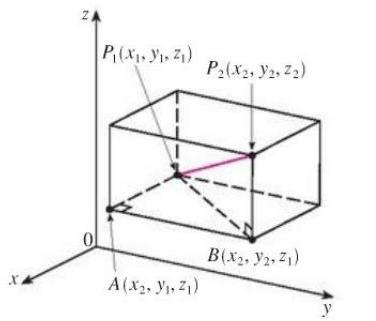
\includegraphics[scale=0.5]{3D-distance.jpg}
\caption{Distances in 3D}
\label{dist}
\end{center}
\end{figure}
\begin{proof}
In Figure \ref{dist}, the pink line represents the distance $|P_1P_2|$, and a rectangular prism is constructed using the two points as opposite vertices. Refer to the figure for points $A,B$ defined above.
\begin{gather*}
    |P_1A| = |x_2-x_1|\hspace{35pt}|AB| = |y_2-y_1|\hspace{35pt}|BP_2| = |z_2-z_1|
\end{gather*}
Using the Pythagorean theorem:
\begin{gather*}
    |P_1P_2|^2 = |P_1B|^2 + |BP_2|^2\\
    |P_1B|^2 = |AB|^2 + |P_1A|^2
\end{gather*}
Now substituting,
\begin{gather*}
    |P_1P_2|^2 = (x_2-x_1)^2+(y_2-y_1)^2+(z_2-z_1)^2\\
    |P_1P_2| = \sqrt{(x_2-x_1)^2+(y_2-y_1)^2+(z_2-z_1)^2}
\end{gather*}
\end{proof}
Applying the distance formula, we can find the equation of a sphere in 3D, since the distance between the center and any point on the sphere is $r$. Squaring both sides of the distance formula with $|P_1P_2| = r$ yields the formula of a sphere with center $C(h,k,l)$.
\begin{gather*}
    (x-h)^2 + (y-k)^2 + (z-l)^2 = r^2
\end{gather*}
\subsection{Vectors}
A \textbf{vector} is any quantity that can be described by a magnitude and a direction. Vectors are often represented by a line that has a direction(indicated with an arrow) and a magnitude(indicated by the length). The notation for vectors here will be: $\vv{AB}$ for a vector with \textbf{initial point} $A$ and \textbf{terminal point} $B$. The magnitude of this vector is $|\vv{AB}|$.

If two vectors $\vv{u}$ and $\vv{v}$ have the same magnitude and direction, they are considered equal. The \textbf{Zero Vector} is a vector with magnitude $0$ and no direction.
\subsubsection{Vector Operations}
If a particle moves along a displacement vector $\vv{AB}$ and another one $\vv{BC}$, then it's total displacement is called the \textbf{sum} of the vectors:
\begin{gather*}
    \vv{AC} = \vv{AB} + \vv{BC}
\end{gather*}
Visually, this \textbf{resultant} vector can be found by positioning the two vectors head to tail and drawing from the first head to the last tail as seen in Fig. \ref{vecadd}.
\begin{figure}[H]
\begin{center}
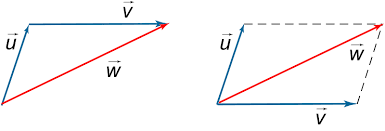
\includegraphics[scale=0.5,angle=2]{vectoraddition.png}
\caption{Vector Addition}
\label{vecadd}
\end{center}
\end{figure}
The resultant $\vv{w}$ can also be obtained by starting both vectors at the same point and drawing the diagonal of the parallelogram indicated in Fig. \ref{vecadd}. Note how the parallelogram can also show that vector addition is commutative.

\textbf{Scalar Multiplication} is multiplying any vector $\vv{v}$ by a constant $c$, forming a new vector $c\vv{v}$. Scalar Multiplication multiplies the magnitude of the vector by $c$. Remember a \textbf{scalar} is a vector with no direction.

The new vector $c\vv{v}$'s magnitude is equal to $c|\vv{v}|$ and it's direction is the same as $\vv{v}$ when $c > 0$ and the opposite when $c < 0$. Notice how $c\vv{v}$ has the same direction as $\vv{v}$ when $c > 0$.

The \textbf{negative} of $\vv{v}$ is $-\vv{v}$, simply $\vv{v}$ in the opposite direction. \textbf{Vector Subtraction} can be defined similar to algebraic subtraction:
\begin{gather*}
    a - b = a + (-b)\\
    \vv{u} - \vv{v} = \vv{u} + (-\vv{v})
\end{gather*}
\begin{figure}[H]
\begin{center}
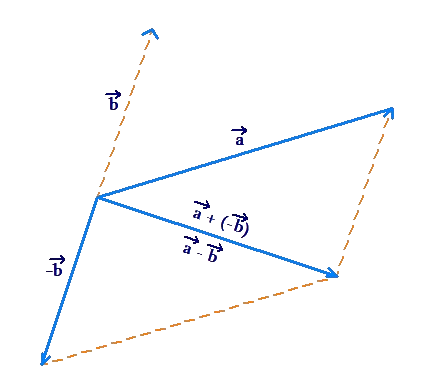
\includegraphics[scale=0.5,angle=0]{vecsub.png}
\caption{Vector Subtraction}
\label{vecsub}
\end{center}
\end{figure}
In Fig \ref{vecsub}, it can be seen how this works. Also, by lining up $\vv{a}$ and $\vv{b}$ at the same starting point, the vector connecting their tails is $\vv{a} - \vv{b}$. Notice how here subtraction is \textit{not} commutative.
\subsubsection{Components and Resultants}
To use vector mathematically, it makes sense to introduce a coordinate system. By convention, the vector starts at the origin and since 2 points define a line, only 2(or 3 in 3D) coordinates are needed to define a vector:
\begin{gather*}
    \vv{v} = \langle a,b \rangle
\end{gather*}
$\langle \rangle$ are used instead of $()$ to show that this is a vector and not a point. This representation from the origin to a particular point makes $\vv{v}$ a \textbf{position vector}.

If the vector doesn't start at the origin, and instead goes between two points $A(x_1,y_1,z_1)$ and $B(x_2,y_2,y_2)$ then:
\begin{gather*}
    \vv{AB} = \vl x_2 - x_1, y_2 - y_1, z_2 - z_1 \vr
\end{gather*}
Remember the magnitude of a vector is the length of its line representation, so using the Pythagorean Theorem in coordinates:
\begin{gather*}
    |\vv{v}| = \sqrt{(v_x)^2 + (v_y)^2}
\end{gather*}
Thinking about the vector addition triangle, to add/subtract two vectors, just add/subtract their components(coordinates). The same works for scalar multiplication, because of similar triangles(scaling up).

Sometimes vectors need to be greater than three dimensions, and so to represent $n$-dimensional vectors, the set $V_n$ represents the set of all possible $n$-dimensional vectors:
\begin{gather*}
    \vv{v_n} = \vl x,y,z...n \vr \in V_n
\end{gather*}
\subsubsection{Vector Properties}
\begin{gather}
    \vv{a} + \vv{b} = \vv{b} + \vv{a}\\
    \vv{a} + 0 = \vv{a}\\
    c(\vv{a} + \vv{b}) = c\vv{a} + c\vv{b}\\
    (\vv{a} + \vv{b}) + \vv{c} = \vv{a} + (\vv{b} + \vv{c})\\
    \vv{a} - \vv{a} = \vv{a} + -\vv{a} = 0\\
    (c+d)\vv{a} = c\vv{a} + c\vv{b}
\end{gather}
These are easily proved, either algebraically or geometrically.
\subsubsection{Unit Vectors}
Consider three 3D vectors:
\begin{gather*}
    \hat{i} = \vl 1,0,0 \vr\hspace{35pt}\hat{j} = \vl 0,1,0 \vr\hspace{35pt}\hat{k} = \vl 0,0,1 \vr
\end{gather*}
These \textbf{unit vectors} all have magnitude $1$ and point in the $x,y,z$ directions. This is interesting because any vector can now be written as scalar multiples of unit vectors:
\begin{gather*}
    \vv{v} = \vl x,y,z \vr = \vl x,0,0 \vr + \vl 0,y,0 \vr + \vl 0,0,z \vr = x\hat{i} + y\hat{j} + z\hat{k}
\end{gather*}
In essence, this notation represents any vector as the vector sum of its components in the $x,y,z...n$ directions.

In general, if $|\vv{v}| \neq 0$, then the unit vector $\hat{u}$ in the $v$-direction is:
\begin{gather*}
    \hat{u} = \dfrac{\vv{v}}{|\vv{v}|}
\end{gather*}
To show why this is true:
\begin{gather*}
    \vv{v} = |\vv{v}|\hat{u}\\
    \hat{u} = \dfrac{\vv{v}}{|\vv{v}|}
\end{gather*}
This is true since $|\vv{v}|$ is a scalar quantity.
\subsection{The Dot Product}
Addition, Subtraction, and Scalar Multiplication are possible, but can you multiply a vector by another vector? One way to do it is called the \textbf{dot product}.

Given $\vv{a} = \vl x_1,y_1,z_1 \vr$ and $\vv{b} = \vl x_2,y_2,z_2 \vr$, the dot product of these is:
\begin{gather*}
    \vv{a} \vdot \vv{b} = x_1x_2 + y_1y_2 + z_1z_2
\end{gather*}
Note that the dot product is \textit{not a vector} but simply a number(scalar). As a result, this product is often called the \textbf{scalar product}.

Some properties of the dot product are similar to numbers:
\begin{gather}
    \vv{a} \vdot \vv{a} = |\vv{a}|^2\\
    \vv{a} \vdot \vv{b} = \vv{b} \vdot \vv{a}\\
    \textrm{\textbf{0}} \vdot \vv{a} = 0
\end{gather}
These can be proved easily by looking at the vector coordinates. They should also make sense. Associative Property also works here(not shown).
\subsubsection{Visualizing the Dot Product}
The dot product of two vectors that start at the same point can be given in terms of the angle $\theta$ between them, where $\theta \in [0,\pi]$. This should make sense, because if $\theta > \pi$ then there would be a smaller angle on the other side(think reflex angles). This new definition is used a lot more in physics(ex. work):
\begin{gather*}
    \vv{a} \vdot \vv{b} = |\vv{a}||\vv{b}|cos(\theta)
\end{gather*}
\begin{proof}
Imagine a triangle $\Delta ABO$ where $OA,OB,AB$ represent $\vv{a},\vv{b},\vv{a}-\vv{b}$ respectively. Applying the law of cosines to $\theta = \measuredangle BOA$:
\begin{gather*}
    |\vv{a} - \vv{b}|^2 = |\vv{a}|^2 + |\vv{b}|^2 - 2|\vv{a}||\vv{b}|cos(\theta)\\
    (\vv{a} - \vv{b})\vdot(\vv{a} - \vv{b}) = \vv{a} \vdot \vv{a} + \vv{b} \vdot \vv{b} - 2|\vv{a}||\vv{b}|cos(\theta)\\
    \vv{a} \vdot \vv{a} - \vv{a} \vdot \vv{b} - \vv{b} \vdot \vv{a} + \vv{b} \vdot \vv{b} = \vv{a} \vdot \vv{a} + \vv{b} \vdot \vv{b} - 2|\vv{a}||\vv{b}|cos(\theta)\\
    -2(\vv{a} \vdot \vv{b}) = -2|\vv{a}||\vv{b}|cos(\theta) \implies \vv{a} \vdot \vv{b} = |\vv{a}||\vv{b}|cos(\theta)
\end{gather*}
\end{proof}
Using this we can conclude:
\begin{gather*}
    cos(\theta) = \dfrac{\vv{a} \vdot \vv{b}}{|\vv{a}||\vv{b}|}
\end{gather*}
Now since $\theta$ is the angle in between $\vv{a}$ and $\vv{b}$, these vectors are \textbf{perpendicular} or \textbf{orthogonal} if the angle between them is $90^{\circ} = \frac{\pi}{2}$ which leads to:
\begin{gather*}
    \vv{a} \vdot \vv{b} = |\vv{a}||\vv{b}|cos\bigg(\dfrac{\pi}{2}\bigg) = 0
\end{gather*}
So two vectors are \textbf{orthogonal} if and only if their dot product $= 0$.
\subsubsection{Direction Angles and Direction Cosines}
The \textbf{direction angles} of any nonzero vector $\vv{v}$ are the specific angles $\alpha,\beta,\gamma \in [0,\pi]$ that $\vv{v}$ makes with the positive $xyz$ axes. The cosines of these angles are called \textbf{direction cosines}.
\begin{gather*}
    cos(\alpha) = \dfrac{\vv{a} \vdot \hat{i}}{|\vv{a}||\hat{i}|} = \dfrac{\vl x_1,y_1,z_1 \vr \vdot \vl 1,0,0 \vr}{|\vv{a}|*1} = \dfrac{x_1}{|\vv{a}|}
\end{gather*}
Similarly:
\begin{gather*}
    cos(\beta) = \dfrac{y_1}{|\vv{a}|}\hspace{45pt}cos(\gamma) = \dfrac{z_1}{|\vv{a}|}
\end{gather*}
By squaring all expressions and using $(x_1)^2 + (y_1)^2 + (z_1)^2 = |a|^2$(dist. formula):
\begin{gather*}
    cos^2(\alpha) + cos^2(\beta) + cos^2(\gamma) = 1
\end{gather*}
Also, because of scalar multiplication:
\begin{gather*}
    \vv{a} = \vl x_1,y_1,z_1 \vr = \vl |\vv{a}|cos(\alpha),|\vv{a}|cos(\beta),|\vv{a}|cos(\gamma) \vr = |\vv{a}|\vl cos(\alpha),cos(\beta),cos(\gamma)\vr\\
    \dfrac{\vv{a}}{|\vv{a}|} = \vl cos(\alpha),cos(\beta),cos(\gamma)\vr = \hat{a}
\end{gather*}
So the vector made up of direction cosines of $\vv{a}$ is the unit vector in the \textbf{a}-direction, which makes sense since $cos(\theta) = 1 * cos(\theta)$, and $|\hat{a}| = 1$
\subsubsection{Projections}
\begin{figure}[H]
\begin{center}
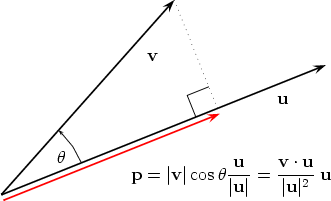
\includegraphics[scale=0.5,angle=0]{vecproj.png}
\caption{Vector Projections}
\label{vecproj}
\end{center}
\end{figure}
The figure above shows a \textbf{vector projection}, which is the vector component of $\vv{v}$ in the $\vv{u}$ direction, and it is represented by $\vv{p}$. It is obtained by first taking a \textbf{scalar projection}, which is the component of $\vv{v}$ along $\vv{u} = |\vv{v}|cos(\theta)$ and multiplying that by $\hat{u} = \frac{\vv{u}}{|\vv{u}|}$, the unit vector in the u-direction.
\begin{gather*}
    comp_a \vv{b} = \dfrac{\vv{a}}{|\vv{a}|}|\vv{b}|*cos(\theta) = \dfrac{\vv{a} \vdot \vv{b}}{|\vv{a}|}\\
    proj_a \vv{b} = \hat{a}*comp_a \vv{b} = \dfrac{\vv{a}}{|\vv{a}|}\bigg[\dfrac{\vv{a} \vdot \vv{b}}{|\vv{a}|}\bigg] = \vv{a}\bigg[\dfrac{\vv{a} \vdot \vv{b}}{|\vv{a}|^2}\bigg]
\end{gather*}
\subsection{The Cross Product}
A second type of vector product is called the \textbf{cross product}. However this time the product is not a scalar but an actual vector, and the cross product is often called the \textbf{vector product}.
\subsubsection{Cross Products and Determinants}
If $\vv{a} = \vl x_1,y_1,z_1 \vr$ and $\vv{b} = \vl x_2, y_2, z_2\vr$, then their cross product $\vv{a} \times \vv{b}$ is:
\begin{gather*}
    \vv{a} \times \vv{b} = \vl y_1z_2 - z_1y_2, z_1x_2 - x_1z_2, x_1y_2 - y_1x_2 \vr
\end{gather*}
This is an interesting product for one because $\vv{a} \times \vv{b}$ will always be $\perp$ to $\vv{a}$ and $\vv{b}$(shown later). Notice that cross products are only defined for 3D vectors $\vv{a}$ and $\vv{b}$.

Cross products are often denoted using \textbf{determinants}, for example an order 2 determinant:
\begin{gather*}
    \begin{vmatrix}
    a & b\\
    c & d
    \end{vmatrix}
    \implies
    \det
    \begin{pmatrix}
    a & b\\
    c & d
    \end{pmatrix}
    = ad - bc
\end{gather*}
Now an order 3 determinant can be defined with order 2 determinants:
\begin{gather*}
\det
    \begin{vmatrix}
    x_1 & x_2 & x_3\\
    y_1 & y_2 & y_3\\
    z_1 & z_2 & z_3
    \end{vmatrix}
    =
    x_1
    \begin{vmatrix}
    y_2 & y_3\\
    z_2 & z_3
    \end{vmatrix}
    - x_2
    \begin{vmatrix}
    y_1 & y_3\\
    z_1 & z_3
    \end{vmatrix}
    + x_3
    \begin{vmatrix}
    y_1 & y_2\\
    z_1 & z_2
    \end{vmatrix}
\end{gather*}
Notice how this works: For every $x_i$ in column $i$, $x_i$ is multiplied by the order 2 determinant found when the $x$-row and column $i$ are both deleted.

Now for cross products, when two vectors $\vv{a} = x_1\hat{i} + x_2\hat{j} + x_3\hat{k}$ and $\vv{b} = y_1\hat{i} + y_2\hat{j} + y_3\hat{k}$, their cross product is shown in this determinant:
\begin{gather*}
    \vv{a} \times \vv{b} =
    \begin{vmatrix}
    x_2 & x_3\\
    y_2 & y_3
    \end{vmatrix}
    \hat{i} -
    \begin{vmatrix}
    x_1 & x_3\\
    y_1 & y_3
    \end{vmatrix}
    \hat{j} +
    \begin{vmatrix}
    x_1 & x_2\\
    y_1 & y_2
    \end{vmatrix}
    \hat{k}
    =
    \begin{vmatrix}
    \hat{i} & \hat{j} & \hat{k}\\
    x_1 & x_2 & x_3\\
    y_1 & y_2 & y_3
    \end{vmatrix}
\end{gather*}
One interesting consequence of the cross product is that $\vv{a} \times \vv{b}$ is orthogonal(perpendicular) to $\vv{a}$ and $\vv{b}$. For this to even be possible for any vectors $\vv{a}$ and $\vv{b}$, this must take place in $V_3$.
\begin{proof}
This is easily proved by showing that $(\vv{a} \times \vv{b}) \vdot \vv{a} = 0$ and also for $\vv{b}$.
\end{proof}
\subsubsection{Visualizing Cross Products}
$\vv{a} \times \vv{b}$ is perpendicular to the plane of $\vv{a}$ and $\vv{b}$, and so it is always perpendicular to both vectors. To find if $\vv{a} \times \vv{b}$ points up or down, use the \textbf{right hand rule} with fingers curling in the direction of rotation from $\vv{a}$ to $\vv{b}$ on the smaller angle($\leqslant 180^{\circ})$.

To find the magnitude of the cross product: Given $\theta$, the angle between $\vv{a}$ and $\vv{b}$(the smaller one):
\begin{gather*}
    |\vv{a} \times \vv{b}| = |\vv{a}||\vv{b}|\sin(\theta)
\end{gather*}
\begin{proof}
Expand the vector coordinates to show that:
\begin{gather*}
    |\vv{a} \times \vv{b}|^2 = |\vv{a}|^2|\vv{b}|^2(1 - \cos^2(\theta)) = |\vv{a}|^2|\vv{b}|^2\sin^2(\theta)
\end{gather*}
\end{proof}
Note in this proof that square root of both sides yields $\sqrt{\sin^2(\theta)} = |\sin(\theta)| = \sin(\theta)$ for all $\theta \in [0,\pi]$.

Using this, two nonzero vectors are parallel if and only if $\vv{a} \times \vv{b} = 0$, because $\vv{a} \times \vv{b} = 0$ when $\theta = 0^{\circ}$ or $180^{\circ}$, which only happens when $\vv{a} \parallel \vv{b}$.
\subsubsection{Interpreting the Cross Product}
One interpretation of the magnitude of the cross product is here:
\begin{figure}[H]
\begin{center}
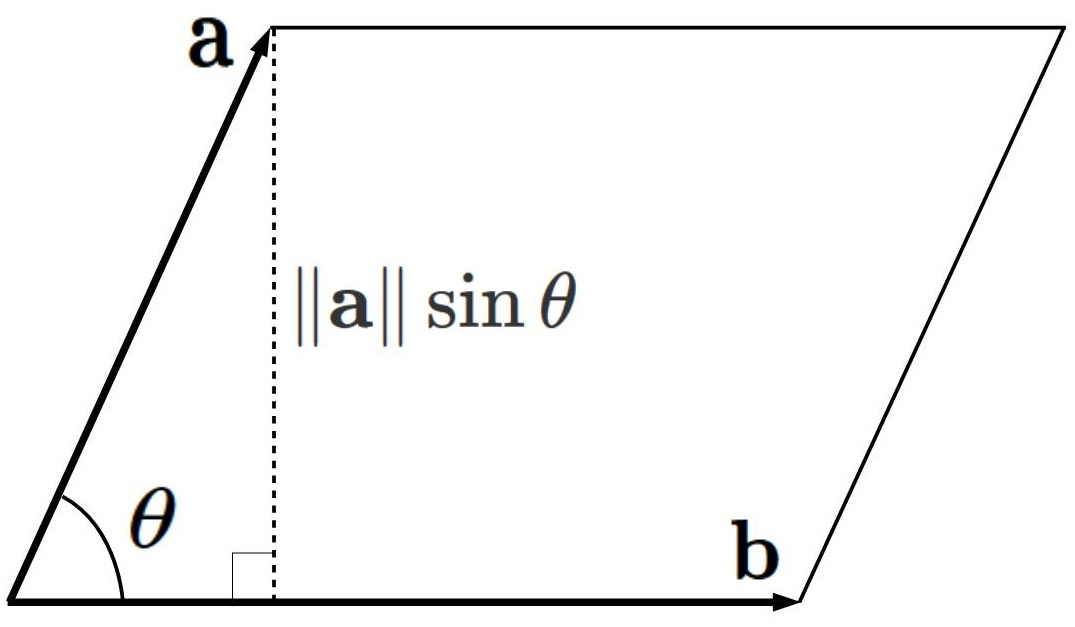
\includegraphics[scale=0.15,angle=0]{crossarea.jpg}
\caption{Area of a Parallelogram}
\label{crossarea}
\end{center}
\end{figure}
In Figure \ref{crossarea}, the area of a parallelogram formed by two vectors $\vv{a}$ and $\vv{b}$ is shown. This area can be expressed as:
\begin{gather*}
    A = Bh = |\vv{b}|*h = |\vv{b}|*(|\vv{a}|\sin(\theta)) = |\vv{a} \times \vv{b}|
\end{gather*}
Notice how the area is $|\vv{a} \times \vv{b}|$ not $\vv{a} \times \vv{b}$. This is because the cross product is a vector, and also in general $\vv{a} \times \vv{b} \neq \vv{b} \times \vv{a}$. These two products will have the same magnitude but will point in opposite directions(right hand rule).

Also, because the cross product is always perpendicular to both vectors:
\begin{gather*}
    \hat{i} \times \hat{j} = \hat{k}\hspace{75pt}\hat{j} \times \hat{i} = -\hat{k}
\end{gather*}
These unit vectors will be perpendicular to each other, also notice how $\hat{k}$ and $-\hat{k}$ point in opposite directions but both have a magnitude of $1$.

Notice how(determinants):
\begin{gather*}
    \vv{a} \vdot (\vv{b} \times \vv{c}) =
    \begin{vmatrix}
    a_1 & a_2 & a_3\\
    b_1 & b_2 & b_3\\
    c_1 & c_2 & c_3
    \end{vmatrix}
\end{gather*}
This combined product is called a \textbf{scalar triple product}, because it combines three vectors into a single scalar. Now why is this important? Refer to the figure below:
\begin{figure}[H]
\begin{center}
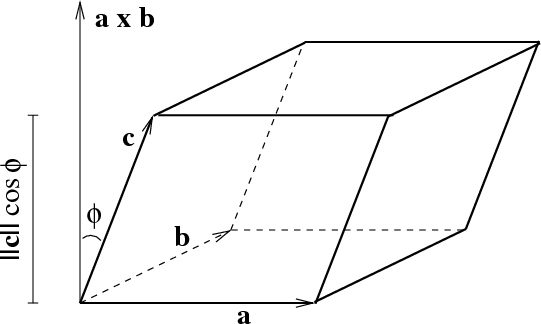
\includegraphics[scale=0.3,angle=0]{crossvol.png}
\caption{Volume of a  Parallelepiped}
\label{crossvol}
\end{center}
\end{figure}
We know from Figure \ref{crossarea} that the base of this figure is a parallelogram with area $|\vv{a} \times \vv{b}|$.
\begin{gather*}
    V = Ah = |\vv{a} \times \vv{b}|h = |\vv{a} \times \vv{b}||\vv{c}|\cos(\phi) = |\vv{c} \vdot (\vv{a} \times \vv{b})|
\end{gather*}
Notice how this is a form of the scalar triple product. Also note that if the volume determined this way is zero, then all three vectors must lie in the same plane, since $\vv{a} \times \vv{b} \perp \vv{c}$.
\subsubsection{Applications}
One application of the cross product is in physics, in torque for example:
\begin{gather*}
    \vv{\tau} = \vv{r} \times \vv{F}
\end{gather*}
This is because the only force that can turn something is the component of it that is perpendicular to the $\vv{r}$. This is also why the direction of a torque can be found using the right hand rule.
\subsection{Equations of Lines and Planes}
Equipped with cross and dot products, we can come up with new definitions in geometry, that are easier to use in 3D space.
\subsubsection{Lines}
A line can be determined in a plane by giving a point and a direction(slope), which is how point-slope form works. Similarly, a 3D line can be defined using a point $P_0(x_0,y_0,z_0)$ and a direction, which here takes the form of a vector $\vv{v}$ parallel to the line. Now draw position vectors $\vv{r_0}$ and $\vv{r}$ to $P_0$ and $P(x,y,z)$ which will represent any point on the line. Now imagine a final vector $\vv{a}$ which goes between $P$ and $P_0$ on the line, and since both \textbf{$r$}-vectors start on the same point:
\begin{gather*}
    \vv{a} = \vv{r} - \vv{r_0}\\
    \vv{r} = \vv{r_0} + \vv{a}
\end{gather*}
Since $\vv{a}$ is on the line, $\vv{a}$ and $\vv{v}$ are parallel, which means $\vv{a} = \vv{v}t$ for some scalar $t$(both vectors point in the same direction but have different lengths).
\begin{gather*}
    \vv{r} = \vv{r_0} + \vv{v}t
\end{gather*}
This is the \textbf{vector equation} of the line. The line is traced out as the \textbf{parameter} $t$ varies. When $t > 0$, $\vv{r}$ traces on one side of $P_0$ and when $t < 0$, $\vv{r}$ traces the other side.

Rewriting $\vv{v} = \vl a,b,c \vr$, then $\vv{v}t = \vl ta, tb, tc\vr$. For our two position vectors $\vv{r} = \vl x,y,z \vr$ and $\vv{r_0} = \vl x_0, y_0, z_0 \vr$ so:
\begin{gather*}
    \vl x,y,z \vr = \vl x_0 + at, t_0 + bt, z_0 + ct \vr
\end{gather*}
Finally, equating components:
\begin{gather*}
    x = x_0 + at\hspace{30pt}y = y_0 + bt\hspace{30pt}z = z_0 + ct
\end{gather*}
These are called \textbf{parametric equations}(can you see why?) and they trace out a line, as each value of $t$ gives a point $(x,y,z)$ on the line. Notice the similarity between this and $y = mx + b$.

Notice how any vector $\vv{v}$ parallel to the line could be used(with any magnitude) and the same line will be formed. If we use $\vv{v} = \vl a,b,c \vr$ then the numbers $a,b,c$ are called the \textbf{direction numbers} of the line. Since any magnitude of $\vv{v}$ could be used, the same line will be formed if $\vv{v} = \vl na, nb, nc \vr$.

We can eliminate the parameter $t$ from all parametric equations by solving for it and substituting:
\begin{gather*}
    \dfrac{x-x_0}{a} = \dfrac{y - y_0}{b} = \dfrac{z - z_0}{c}
\end{gather*}
for $a,b,c \neq 0$. These non-parametric equations are called the \textbf{symmetric equations} of the line. However, as long as at least one of the direction numbers are not zero, this can be used. Ex. if $a = 0$, then $x = x_0 + (0)t$ and:
\begin{gather*}
    x = x_0\hspace{60pt}\dfrac{y-y_0}{b}=\dfrac{z-z_0}{c}
\end{gather*}
This also shows that the line lies on the plane $x = x_0$(in 3D space).

Since $\vv{v} = \vl a,b,c \vr$, and $\vv{v}$ can be the vector drawn between any two points $P(x_0,y_0,z_0)$ and $P_1(x_1,y_1,z_1)$:
\begin{gather*}
    \vv{v} = \vl a,b,c \vr = \vl x_1 - x_0,y_1-y_0,z_1-z_0 \vr\\
    a = x_1 - x_0\hspace{25pt}b = y_1 - y_0\hspace{25pt}c = z_1-z_0\\
    \dfrac{x - x_0}{x_1 - x_0} = \dfrac{y - y_0}{y_1 - y_0} = \dfrac{z - z_0}{z_1 - z_0}
\end{gather*}
This can also be used as an equation of a line. Notice how you can derive the point slope form of a line from this. If you want to define a \textbf{line segment} instead of a whole line, restrict the parameter $t$.

In fact, if you need to find a line segment between two points $P_0$ and $P_1$, find position vectors $\vv{r_0}$ and $\vv{r_1}$ respectively. Since both position vectors have tips on the line and start at the same point, we can choose $\vv{v} = \vv{r_1} - \vv{r_0}$:
\begin{gather*}
    \vv{r} = \vv{r_0} + \vv{v}t = \vv{r_0} + (\vv{r_1}-\vv{r_0})t = \vv{r_0}(1-t) + \vv{r_1}t
\end{gather*}
As $t$ ranges from $0$ to $1$, $\vv{r}$ traces out the correct line segment between $P_0$ and $P_1$.
\subsubsection{Planes}
To define a plane, a single parallel vector is not enough. However, with a orthogonal($\perp$) vector and an initial point(a plane could be defined as all points perpendicular to the vector on the same "level" as the initial point. This vector $\vv{n}$ is called the \textbf{normal vector}. Let $P_0(x_0,y_0,z_0)$ be the initial point and $P(x,y,z)$ be any point on the plane. Define position vectors $\vv{r}$ and $\vv{r_0}$. Since $\vv{r}$ and $\vv{r_0}$ start at the same point, $\vv{r} - \vv{r_0}$ will also be on the plane orthogonal to $\vv{n}$:
\begin{gather*}
    \vv{n} \vdot (\vv{r} - \vv{r_0}) = 0\\
    \vv{n} \vdot \vv{r} = \vv{n} \vdot \vv{r_0}
\end{gather*}
If $\vv{n} = \vl a,b,c \vr$, $\vv{r} = \vl x,y,z \vr$ and $\vv{r_0} = \vl x_0,y_0,z_0 \vr$:
\begin{gather*}
    \vl a,b,c \vr \vdot \vl x-x_0,y-y_0,z-z_0 \vr = 0\\
    a(x-x_0) + b(y-y_0) + c(z-z_0) = 0
\end{gather*}
This is the \textbf{scalar equation} of a plane. Notice that if $a,b,c$ are not all $0$ then the equation of a plane can take the form:
\begin{gather*}
    ax + by + cz + d = 0
\end{gather*}
The great thing about normal vectors is that they act as "markers" for planes. For example, two planes with normals $\vv{n_1}$ and $\vv{n_2}$ are parallel if their vectors are parallel, in other words is $\vv{n_2} = c\vv{n_1}$, where $c$ is a constant. If they aren't parallel, then they intersect in a line and the angle between the two planes($< 90^{\circ}$ is the angle between their vectors(use dot product).

Since the intersection of two planes is a line, a line can be written as the intersection of two planes.
\begin{gather*}
    \dfrac{x-x_0}{a} = \dfrac{y-y_0}{b}\hspace{45pt}\dfrac{y-y_0}{b} = \dfrac{z-z_0}{c}
\end{gather*}
These two equations are equations of planes, and when set equal become an equation of a line!

Lastly, the distance between two \textit{parallel} planes is:
\begin{gather*}
    D = \dfrac{|ax_1 + by_1 + cz_1 + d|}{\sqrt{a^2 + b^2 + c^2}}
\end{gather*}
This can be found by finding the projection of a vector between one point on each plane on their \textit{shared} normal vector.
\subsection{Cylinders and Quadric Surfaces}
Planes are a more simple type of surface, and graphing those are not too difficult. However, in more complex surfaces it is often useful to get the cross sections of the surface on different planes, which are called \textbf{traces}.
\subsubsection{Cylinders}
A cylinder is a type of surface that is made up of a set of lines(called \textbf{rulings}) that are all parallel to a given(central) line and pass through a curved plane. Note that a cylinder does not always have to be the cylinder you're thinking of(see \textbf{parabolic cylinder}).
\subsubsection{Quadric Surfaces}
A \textbf{quadric surface} is the result of a degree 2 polynomial equation written in $x,y,z$:
\begin{gather*}
    ax^2 + by^2 + cz^2 + dxy + eyz + fxz + gx + hy + Iz + j = 0
\end{gather*}
Quadric surfaces are the 3D equivalent to the 2D conics(see 11.5)
\subsubsection{Sketching Surfaces}
The main method for sketching surfaces is to use traces(cross-sections) that are parallel to the $xyz$ planes. For example, to graph:
\begin{gather*}
    \dfrac{x^2}{a^2} + \dfrac{y^2}{b^2} + \dfrac{z^2}{c^2} = 1
\end{gather*}
First find the traces in each direction, by substituting $x=k$ then $y=k$ and finally $z=k$, where $k$ is any number. This simplifies the 3D surface into a bunch of slices of 2D curves.
\begin{gather*}
    \dfrac{x^2}{a^2} + \dfrac{y^2}{b^2} = 1 - \dfrac{k^2}{c^2}
\end{gather*}
This is an example of $z = k$, where every term on the right side is a constant, which means that when $k^2 < c^2$ then the right side is $< 1$ and the trace is an ellipse.
\subsection{Cylindrical and Spherical Coordinates}
In 3D, polar coordinates are expressed in two different but useful coordinate systems.
\subsubsection{Cylindrical Coordinates}
In \textbf{cylindrical coordinates} any point in 3D space can be represented by three numbers $(r,\theta,z)$ where $r$ and $\theta$ are the polar coordinates of the point on 2D space(on the $xy$ plane), and $z$ is the $z$-coordinate of the point.
\begin{figure}[H]
\begin{center}
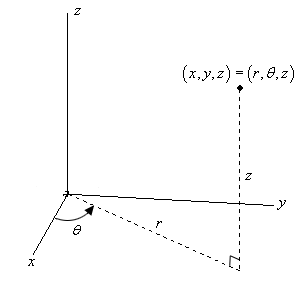
\includegraphics[scale=0.6,angle=0]{cylcoords.png}
\caption{Cylindrical Coordinates}
\label{cylcoords}
\end{center}
\end{figure}
To convert from cylindrical to rectangular:
\begin{gather*}
    x = r\cos(\theta)\hspace{20pt}y=r\sin(\theta)\hspace{20pt}z=z
\end{gather*}
To convert back to rectangular:
\begin{gather*}
    r^2 = x^2 + y^2\hspace{20pt}\tan(\theta) = \dfrac{y}{x}\hspace{20pt}z=z
\end{gather*}
Cylindrical coordinates are the best to choose when dealing with symmetry about a certain axis(especially the $z$-axis). Imagine a cylinder around the $z$-axis $x^2 + y^2 = c^2$. In cylindrical coordinates, that equation is $r=c$, since $\theta$ and $z$ can vary to create the cylinder.
\subsubsection{Spherical Coordinates}
\begin{figure}[H]
\begin{center}
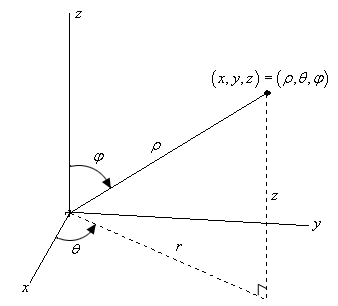
\includegraphics[scale=0.6,angle=0]{spherical.png}
\caption{Spherical Coordinates}
\label{sphcoords}
\end{center}
\end{figure}
The \textbf{spherical coordinates} of a point in 3D can be described using $(\rho, \theta, \phi)$, where $\rho = |OP|$(dist. from origin to $P$) and $\theta$ is the same angle in cylindrical. $\phi$ is the angle between $\rho$ and the $z$-axis.
\begin{gather*}
    \rho \geqslant 0\hspace{25pt}0 \leqslant \phi \leqslant \pi
\end{gather*}
This coordinate system is useful when dealing with symmetry about a point. Easiest way to see this is with a sphere, with equation $\rho = c$, since $\theta$ and $\phi$ can vary wildly, drawing out a sphere with all points a distance $\rho = c$ away from the origin.

Some common spherical coordinate uses are $\theta = c$(a half plane), $\phi = c$, a cone above the $xy$ plane when $c \in [0, \frac{\pi}{2}]$ and below when $c \in [\frac{\pi}{2},\pi]$.

To convert from spherical to rectangular, refer to Figure \ref{sphcoords}, and imagine points $P(x,y,z)$, $Q$, which is when a line is drawn straight from $P$ to the $z$-axis, and $P'$, which is when a line is drawn straight down from $P$ to the $xy$ plane. Using the Alt. Interior Angle theorem, the angle between $\rho$ and $z$ in the figure is $\phi$:
\begin{gather*}
    z = \rho\cos(\phi)\hspace{20pt}x = r\cos(\theta) = \rho\sin(\phi)\cos(\theta)\hspace{20pt}y = r\sin(\theta) = \rho\sin(\phi)\sin(\theta)
\end{gather*}
Finally, to convert from rectangular to spherical, use the distance formula(along with the above):
\begin{gather*}
    \rho^2 = x^2 + y^2 + z^2
\end{gather*}
\section{Vector Functions}
\subsection{Vector Functions and Space Curves}
\subsubsection{Limits and Continuity}
Since a function in a basic sense is a mapping of one element of the \textbf{domain} to another element in the \textbf{range}, a \textbf{vector-valued function} is a mapping from a scalar domain to a vector range. In simple terms, every number $t$ in the domain can be mapped to some vector in $V_3$ defined as $\vv{r} = \ve{f(t),g(t),h(t)}$, where $f,g$ and $h$ are the \textbf{component functions} of $\vv{r}$:
\begin{gather*}
    \vv{r}(t) = \ve{f(t),g(t),h(t)} = f(t)\hat{i} + g(t)\hat{j} + h(t)\hat{k}
\end{gather*}
As usual, the domain of $\vv{r}(t)$ is the set of all $t$ where $f,g$ and $h$ are defined. The \textbf{limit} of a vector function is simply the limit of it's components:
\begin{gather*}
    \lim_{t \to c} \vv{r}(t) = \ve{\lim_{t \to c} f(t), \lim_{t \to c} g(t), \lim_{t \to c} h(t)}
\end{gather*}
If all limits exist, then the vector function's limit exists. If the limit of $\vv{r}(t)$ is $\vv{L}$, then the magnitude and direction of $\vv{r}(t)$ approaches that of $\vv{L}$ for values close to $c$. Limits of vector functions obey the same laws as real functions do. It follows that:

Any vector function $\vv{r}(t)$ is continuous at $c$ if:
\begin{gather*}
    \lim_{t \to c} \vv{r}(t) = \vv{r}(c)
\end{gather*}
It follows that $\vv{r}(t)$ is continuous if and only if it's components are.
\subsubsection{Space Curves}
Imagine a vector function $\vv{r}$ with components $f,g$ and $h$, which are all continuous. Now imagine a curve C drawn using the set of points:
\begin{gather*}
    x = f(t)\hspace{40pt}y=g(t)\hspace{40pt}z=h(t)
\end{gather*}
Look familiar? Yes, these are \textbf{parametric equations} of the curve C, and the vector $\vv{r}$ traces out C as $t$ varies. These are just like 3D parametric equations! If C fits the case, the C is a \textbf{space curve}.
\subsubsection{Visualizing Space Curves}
Computer drawing with space curves is a good way to visualize it, but when you do not have technology at your disposal it's good to have a way of visualizing these. You can think of the parametric equations as "traces", similar to drawing surfaces.

Another way to visualize space curves is to draw them on surfaces, for example you could visualize a curve of intersection between two cylinders.
\subsection{Derivatives and Integrals of Vector Functions}
\subsubsection{Derivatives}
Because the limit of a vector function is defined similar to a normal function, we can define the derivative similarly as well(since derivatives are based off limits).

The \textbf{derivative} $\vv{r}'$ of a vector function $\vv{r}$:
\begin{gather*}
    \dfrac{d\vv{r}}{dt}=\vv{r}'(t) = \lim_{h \to 0}\dfrac{\vv{r}(t+h) - \vv{r}(t)}{h}
\end{gather*}
Remember that $\vv{r}(t+h)$ and $\vv{r}(t)$ are both position vectors that start at the same point. So $\vv{r}(t+h) - \vv{r}(t)$ is the distance between them because of simple vector subtraction, which can be treated as secant vector on the curve. As $h \to 0$, the secant vector becomes a \textbf{tangent vector} as long as $\vv{r}'(t)$ exists and $\vv{r}'(t) \neq 0$. So now the \textbf{tangent line} is defined as the line parallel to the vector $\vv{v} = \vv{r}'(t)$ that goes through the point of tangency $P$.

The \textbf{unit tangent vector}, or the unit vector in the direction of the tangent:
\begin{gather*}
    \vv{T}(t) = \dfrac{\vv{r}'(t)}{|\vv{r}'(t)|}
\end{gather*}
However, there is an easier way to get the derivative of a vector function. If $\vv{r} = \ve{f(t),g(t),h(t)}$, where $f,g$ and $h$ are differentiable:
\begin{gather*}
    \vv{r}'(t) = \ve{f'(t),g'(t),h'(t)}
\end{gather*}
This is easily shown by applying the limit definition to each component.

The \textbf{second derivative} is simply the derivative of the derivative, or $\vv{r}''(t)$.

A curve of a function $\vv{r}(t)$ is smooth on an interval if $\vv{r}'$ is continuous and $\vv{r}'(t) \neq 0$, except possibly on the endpoints.

Differentiation rules are the same for a vector function as for a normal function. Dot products and cross products of vectors obey the product rule.
\subsubsection{Integrals}
We can apply the same vector derivative logic to integration with limits to Riemann sums:
\begin{gather*}
    \int_a^b \vv{r}(t) dt = \lim_{n \to \infty} \sum_{i = 1}^n \vv{r}(t_i)\Delta t
\end{gather*}
Applying this to each component, we get:
\begin{gather*}
    \int_a^b \vv{r}(t) dt = \Bigg\vl\bigg[\int_a^b f(t) dt\bigg], \bigg[\int_a^b g(t) dt\bigg], \bigg[\int_a^b h(t) dt\bigg]\Bigg\vr
\end{gather*}
The FTC also works with vector functions:
\begin{gather*}
    \int_a^b \vv{r}(t) dt = \bigg[\vv{R}(t)\bigg]_a^b = \vv{R}(b) - \vv{R}(a)
\end{gather*}
where $\vv{R}$ is the antiderivative of $\vv{r}$.
\subsection{Arc Length and Curvature}
\subsubsection{Arc Length}
From chapter 11, the arc length of a 2D curve with parametric equations $x = f(t)$ and $y = g(t)$ between $a$ and $b$ has arc length:
\begin{gather*}
    L = \int_a^b \sqrt{\bigg[f'(t)\bigg]^2 + \bigg[g'(t)\bigg]^2}\d t
\end{gather*}
where $f'$ and $g'$ must be continuous on the interval. This is found by taking the limit of an n-sided inscribed polygon(as $n \to \infty$). Doing the exact same thing with parametric equations $x = f(t), y = g(t), z = h(t)$. If the curve is traced exactly one time from $a$ to $b$:
\begin{gather*}
    L = \int_a^b \sqrt{\bigg[f'(t)\bigg]^2 + \bigg[g'(t)\bigg]^2+\bigg[h'(t)\bigg]^2}\d t\\
    = \int_a^b \sqrt{\bigg[\dfrac{dx}{dt}\bigg]^2 + \bigg[\dfrac{dy}{dt}\bigg]^2+\bigg[\dfrac{dz}{dt}\bigg]^2}\d t\\
    = \int_a^b |\vv{r}'(t)|\d t
\end{gather*}
Even though different \textbf{parametrizations} of a curve C are possible(different parametric equations that show the same curve), the arc length found will be the same.

Let C be a curve given by $\vv{r}(t) = f(t)\hat{i} + g(t)\hat{j} + h(t)\hat{k}$ for $t \in [a,b]$, and C is traced exactly once in the interval. C's \textbf{arc length function}:
\begin{gather*}
    s(t) = \int_a^t |\vv{r}'(u)| \d u = \int_a^t \sqrt{\bigg[\dfrac{dx}{du}\bigg]^2 + \bigg[\dfrac{dy}{du}\bigg]^2+\bigg[\dfrac{dz}{du}\bigg]^2}\d u
\end{gather*}
Taking the derivative of both sides and using FTC:
\begin{gather*}
    \dfrac{ds}{dt} = |\vv{r}'(t)|
\end{gather*}
It is often useful to parametrize a curve \textbf{with respect to arc length} because arc length is a distance, which is not relative(doesn't change depending on your coordinate system). If any curve $\vv{r}(t)$ and $s(t)$, the arc length function is given, then you can solve for $t$ asa fucntion of $s$: $t = t(s)$. Now since $\vv{r} = \vv{r}(t) \implies \vv{r} = \vv{r}(t) = \vv{r}(t(s))$. For example, $\vv{r}(t(3))$ represents the position vector of $\vv{r}$ at the point 3 units of arc length from the starting point.
\subsubsection{Curvature}
If C is a smooth curve defined by $\vv{r}(t)$, then $\vv{r}'(t) \neq 0$, also the unit tangent vector $\vv{T}$, which is the unit of the derivative:
\begin{gather*}
    \vv{T}(t) = \dfrac{\vv{r}'(t)}{|\vv{r}'(t)|}
\end{gather*}
Imagining a curve, the direction of $\vv{T}$ will change fast when the curve is sharply curved, and slower when the curve is straighter. The \textbf{curvature} of C at a point is how fast the curve changes direction at that point. It is the rate of change of the unit tangent with respect to arc length. Arc length is used because as mentioned it doesn't change when parameterized:
\begin{gather*}
    \kappa(t) = |\dfrac{d\vv{T}}{ds}|
\end{gather*}
Using the chain rule:
\begin{gather*}
    \dfrac{d\vv{T}}{dt} = \dfrac{d\vv{T}}{ds}\dfrac{ds}{dt}\\
    \kappa = |\dfrac{d\vv{T}}{ds}| = |\dfrac{\frac{d\vv{T}}{dt}}{\frac{ds}{dt}}| = \dfrac{|\vv{T}'(t)|}{|\vv{r}'(t)|}
\end{gather*}
This can be used to show that small circles have large curvature and large circles have smaller curvature. The curvature of a circle with radius $a$ is:
\begin{gather*}
    \kappa = \dfrac{1}{a}
\end{gather*}
The following is often more convenient to use:
\begin{gather*}
    \kappa(t) = \dfrac{|\vv{r}'(t) \times \vv{r}''(t)|}{|\vv{r}'(t)|^3}
\end{gather*}
\begin{proof}
Since $\vv{T} = \dfrac{\vv{r}'}{|\vv{r}'|}$ and $|\vv{r}'| = \dfrac{ds}{dt}$:
\begin{gather*}
    \vv{r}' = |\vv{r}'|\vv{T} = \dfrac{ds}{dt}\vv{T}\\
\end{gather*}
Taking a derivative(use product rule):
\begin{gather*}
    \vv{r}'' = \dfrac{d^2s}{dt^2}\vv{T} + \dfrac{ds}{dt}\vv{T}'
\end{gather*}
Cross both sides, and use the fact that $\vv{T} \times \vv{T} = 0$:
\begin{gather*}
    \vv{r}' \times \vv{r}'' = \bigg(\dfrac{ds}{dt}\bigg)^2(\vv{T} \times \vv{T}')
\end{gather*}
Since $\vv{T}$ is a unit vector, $|\vv{T}(t)| = 1$. Since $1$ is a constant, $\vv{T}$ is orthogonal to $\vv{T}'$. Also using $|\vv{a} \times \vv{b}| = |\vv{a}||\vv{b}| \sin(\theta)$:
\begin{gather*}
    |\vv{r}' \times \vv{r}''| = \bigg(\dfrac{ds}{dt}\bigg)^2|\vv{T} \times \vv{T}'| = \bigg(\dfrac{ds}{dt}\bigg)^2|\vv{T}||\vv{T}'| = \bigg(\dfrac{ds}{dt}\bigg)^2|\vv{T}'|\\
    |\vv{T}'| = \dfrac{|\vv{r}' \times \vv{r}''|}{(ds/dt)^2} = \dfrac{|\vv{r}' \times \vv{r}''|}{|\vv{r}'|^2}\\
    \kappa = \dfrac{|\vv{T}'|}{|\vv{r}'|} = \dfrac{|\vv{r}' \times \vv{r}''|}{|\vv{r}'|^3}
\end{gather*}
\end{proof}
For the special case of a 2D curve with equation $y = f(x)$, we can use $x$ as the parameter: $\vv{r}(x) = x\hat{i} + f(x)\hat{j}\implies\vv{r}''(x) = f''(x)\hat{j}$. When crossing, since $\hat{i} \times \hat{j} = \hat{k}$, and $\hat{j} \times \hat{j} = 0: \vv{r}' \times \vv{r}'' = f''(x)\hat{k}$. Also noting that the arc length in 2D:
\begin{gather*}
    L = |\vv{r}'(x)| = \sqrt{1 + [f'(x)]^2}\\
    \kappa(x) = \dfrac{|f''(x)|}{[1 + (f'(x))^2]^\frac{3}{2}}
\end{gather*}
\subsubsection{Normal and Binormal Vectors}
At any point on a space curve $\vv{r}(t)$, there will be many vectors orthogonal to $\vv{T}$, but you can find one by noting that $|\vv{T}| = 1$, so $\vv{T'} \perp \vv{T}$. NOTE: \textbf{$\vv{T}'$ is not a unit vector!} But if $\vv{r}'$ is smooth(derivative not zero), the \textbf{unit normal vector} $\vv{N}(t)$, the unit vector of the unit tangent's derivative(a mouthful!):
\begin{gather*}
    \vv{N}(t) = \dfrac{\vv{T}'(t)}{|\vv{T}'(t)|}
\end{gather*}
The vector given by $\vv{B}(t) = \vv{T}(t) \times \vv{N}(t)$ is called the \textbf{binormal vector}. Since it's a cross, it is perpendicular to both $\vv{T}$ and $\vv{N}$.
\begin{figure}[H]
\begin{center}
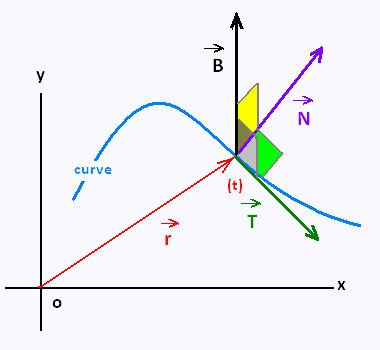
\includegraphics[scale=0.5,angle=0]{tnb.png}
\caption{Tangent, Normal, and Binormal}
\label{tnb}
\end{center}
\end{figure}
The plane defined by $\vv{N}$ and $\vv{B}$ at any point $P$ is called the \textbf{normal plane} at $P$. It contains all lines that are orthogonal to $\vv{T}$. The plane using $\vv{T}$ and $\vv{N}$ is the \textbf{osculating plane} at $P$(\textit{osculum} in Latin means \textit{kiss}). This plane is the closest to containing the part of the curve near $P$. In a 2D curve, this plane is simply the entire plane containing the curve.

The circle that lies in the osculating plane and has the same tangent at $P$, which also lies on the concave side of $C$(the direction $\vv{N}$ points), and has radius $r = \frac{1}{\kappa}$ is the \textbf{osculating circle} at $P$. It best describes how C behaves near $P$, since it shares the same tangent, normal, and curvature.
\subsection{Motion in Space: Velocity and Acceleration}
Tangent and Normal Vectors can be used in physics to study motion, which starts with position, velocity, and acceleration.
\subsubsection{Position, Velocity, and Acceleration}
\begin{gather*}
    \vv{v}(t) = \lim_{h \to 0}\dfrac{\vv{r}(t + h) - \vv{r}(t)}{h}
\end{gather*}
As $h \to 0$, this vector approximates the distance traveled(traced by $\vv{r}$) over a small time interval. And as the limit is taken, this \textbf{velocity} becomes instantaneous. This \textbf{velocity vector} points in the direction of the tangent line(it is the tangent vector).

The \textbf{speed} at time $t$ of a particle is the magnitude of the velocity vector, which makes sense since:
\begin{gather*}
    |\vv{v}(t)| = |\vv{r}'(t)| = \dfrac{ds}{dt}
\end{gather*}
which is the rate of change of distance with respect to time.

In 1 dimension, the \textbf{acceleration} of a particle is the change in velocity:
\begin{gather*}
    \vv{a}(t) = \vv{v}'(t) = \vv{r}''(t)
\end{gather*}
Integrating the vectors allows you to go "backwards":
\begin{gather*}
    \vv{v}(t) = \vv{v}(t_0) + \int_{t_0}^t \vv{a}(t) \d t
\end{gather*}
\subsubsection{Forces}
The equation relating the force, mass, and acceleration experienced by an object is called \textbf{Newton's Second Law} of Motion. If an object in experiences a force $\vv{F}(t)$ with mass $m$ and acceleration $\vv{a}(t)$:
\begin{gather*}
    \vv{F}(t) = m\vv{a}(t)
\end{gather*}
\subsubsection{Tangential and Normal Components}
It is often useful to find the tangential and normal components of the acceleration vector. Using $v$ for speed:
\begin{gather*}
    \vv{T}(t) = \dfrac{\vv{r}'(t)}{|\vv{r}'(t)|} = \dfrac{\vv{v}}{v}\\
    \vv{v} = v\vv{T}
\end{gather*}
Taking the derivative(use Product Rule):
\begin{gather*}
    \vv{a} = \vv{v}' = v'\vv{T} + v\vv{T}'\\
    \kappa = \dfrac{|\vv{T}'|}{|\vv{r}'|} = \dfrac{|\vv{T}'|}{v}\implies |\vv{T}'| = \kappa v
\end{gather*}
Since $\vv{N} = \frac{\vv{T}'}{|\vv{T}'|}$:
\begin{gather*}
    \vv{T}' = |\vv{T}'| \vv{N} = \kappa v \vv{N}\\
    \vv{a} = v'\vv{T} + \kappa v^2 \vv{N}
\end{gather*}
Since both $\vv{T}$ and $\vv{N}$ are unit vectors, their "coefficients" are the components in the tangential and normal directions:
\begin{gather*}
    \vv{a} = a_t \vv{T} + a_n \vv{N}\\
    a_t = v'\hspace{40pt}a_n = \kappa v^2
\end{gather*}
Since there is no third component, this derivation proves that the acceleration of an object must lie in the $\vv{T}\vv{N}$ plane, the \textit{osculating plane}! Now remember that $\vv{T}$ points in the direction of motion(\textit{tangent}) and $\vv{N}$ points in the direction the curve is turning. So the tangential component of $\vv{a}$ is $v'$, which makes sense since in 1 dimension, acceleration is the derivative of velocity.

Another example: If the object is moving in a circle, it's curvature is $\kappa = \frac{1}{r}$. So:
\begin{gather*}
    a_n = \kappa v^2 = \dfrac{1}{r}v^2 = \dfrac{v^2}{r}
\end{gather*}
which is the equation for centripetal acceleration, go figure! Oftentimes, it is easier to work with equations based on position vectors and their derivatives, so:
\begin{gather*}
    \vv{v} \vdot \vv{a} = v\vv{T} \vdot (v' \vv{T} + \kappa v^2 \vv{N})\\
    = vv'\vv{T}\vdot \vv{T} + \kappa v^3 \vv{T} \vdot \vv{N}\\
    = vv'
\end{gather*}
Last step because the dot product of two unit vectors is $1$, and the dot product of orthogonal vectors($\vv{T}$ and $\vv{N}$) is $0$.
\begin{gather*}
    a_t = v' = \dfrac{\vv{v} \vdot \vv{a}}{v} = \dfrac{\vv{r}'(t) \vdot \vv{r}''(t)}{|\vv{r}'(t)|}\\
    a_n = \kappa v^2 = \dfrac{|\vv{r}' \times \vv{r}''|}{|\vv{r}'|^3}|\vv{r}'(t)|^2 = \dfrac{|\vv{r}' \times \vv{r}''|}{|\vv{r}'|}
\end{gather*}
\section{Partial Derivatives}
\subsection{Functions of Several Variables}
In some applications, a function requires a \textit{multivariable} input. This means it takes 2+ variables, such as $T = f(x,y)$. The temperature at a point on Earth requires a latitude and longitude input. The \textbf{domain} of $f$ is the constraints on lat and long($-90,90$ and $-180,180$). The range is the set of possible outputs. If no $D$ or $R$ is given, $D$ is assumed to be all numbers that make the function defined, and $R$ the outputs of $f(x_D,y_D)$.

A function of 2 variables means that the input space is a subset of $\mathbb{R}^2$, a subset of the plane, and then range is a subset of $\mathbb{R}$, a number line.
\subsubsection{Graphs}
Normally, graphing is done similar to single variable functions. Like $y = f(x)$, $z = f(x,y)$. This creates a \textbf{surface}, like an paraboloid.
\begin{figure}[H]
\begin{center}
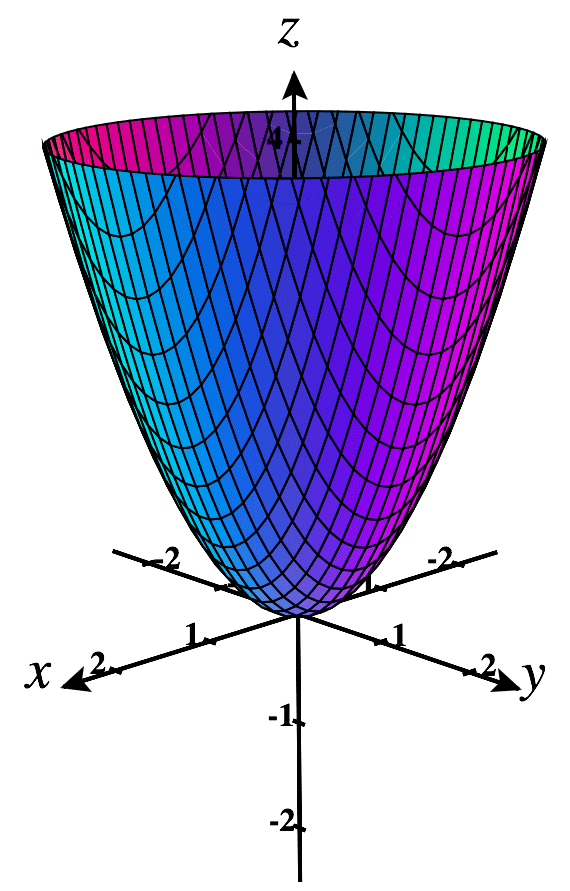
\includegraphics[scale=0.2]{Graphingf.png}
\caption{A Simple Surface}
\label{surface}
\end{center}
\end{figure}
One special function:
\begin{gather*}
    \textrm{\textbf{Linear Multivariable Function: }} f(x,y) = ax + by + c
\end{gather*}
This function forms a plane when graphed.
\subsubsection{Level Curves}
Another way to visualize this type of function is a \textbf{level curve}. Think of traces of a function such that $f(x,y) = k$. This parallels contour maps and helps visualize the peaks and valleys of a function. The surface is steep when the contours are close together and further apart when the surface is shallow(note this steep/shallow does NOT correspond to direct height, just height \textit{change}). These are also similar to lines of electric potential(equipotential lines?).

Note that without numbers you can only see the magnitude of the steepness, not the direction(it could be steep up or steep down).
\subsubsection{Functions of 3+ Variables}
Functions of \textit{three} or more variables are tricky but possible to work with. Using the same temperature example, you could write $T = f(x,y,t)$ where $t$ is now the \textit{time of year}, which is useful.

Notice that the graph of $f(x,y)$ is generated in $3D$. Similarly, the graph of $f(x,y,z)$ is in $4D$ which is very difficult to imagine. However, you can imagine the traces of it like $f(x,y,z) = k$. For example, the function $f(x,y,z) = x^2 + y^2 + z^2$ has traces which are concentric spheres.

For example, to find the total cost of a product which consists of $n$ parts, one could write:
\begin{gather*}
    f(x_1,x_2...x_n) = c_1x_1 + c_2x_2 ... c_nx_n
\end{gather*}
If you write two vectors $\vv{x} = \vl x_1, x_2...x_n \vr$ and $\vv{c}$ similarly, you can rewrite:
\begin{gather*}
    f(\vv{x}) = \vv{c} \vdot \vv{x}
\end{gather*}
\subsection{Limits and Continuity}
Taking an example function:
\begin{gather*}
    f(x,y) = \frac{\sin(x^2-y^2)}{x^2+y^2}
\end{gather*}
As $x$ and $y$ both approach $0$(the origin), we can find that the function approaches $1$. This can be written using multivariable limit notation:
\begin{gather*}
    \lim_{(x,y) \to (0,0)} f(x,y) = 0
\end{gather*}
This means that if you take any path in the domain of $f$ to $(0,0)$, you will approach $1$. You can get as close to the limit $L$ as you want by taking $(a,b)$ sufficiently close to $(0,0)$. The epsilon-delta definition:

Let $f$ be a function of two variables, where the domain has all points \textit{arbitrarily} close to $(a,b)$(a small circle around the point). The \textbf{limit} of $f$ is $L$:
\begin{gather*}
    \lim_{(x,y) \to (a,b)} f(x,y) = L
\end{gather*}
if for every real number $\varepsilon > 0$ there is another number $\delta > 0$ where $f$ is $\varepsilon$ close to $L$ ($|f(x,y) - L| < \varepsilon$) whenever $(x,y)$ is in the domain and $0 < \sqrt{(x-a)^2 + (y-b)^2} < \delta$

Note the final part. That is the distance formula in 2D, from $(x,y)$ to $(a,b)$. This is used because there are multiple directions of approach in 3D functions. Back in 2D you could only approach from left or right. Now you can from any direction, which is why this definition uses \textit{distance}.

In fact, for a limit to be true it must be able to be approached from \textbf{all directions}. If it even fails in one direction then the limit \textbf{does not exist}.
\subsubsection{Existing Limits}
Calculating limits for multivariable functions can be greatly simplified by using limit laws. The squeeze theorem also works(though it's very interesting to squeeze a surface in between two others). Mainly use the epsilon-delta definition and start with:
\begin{gather*}
    |f(x,y) - L| < \varepsilon
\end{gather*}
Then work to find a $\delta$ using inequalities which fits the requirements and constraints given by the function and inequality methods. If you really can't find one it probably doesn't exist.
\subsubsection{Continuity}
A characteristic property of continuity in single variable functions is that $\lim_{x \to a} f(x) = f(a)$, which proves the function of continuous. Similarly, that works here:

A function $f(x,y)$ is \textbf{continuous} at $(a,b)$ if
\begin{gather*}
    \lim_{(x,y) \to (a,b)} f(x,y) = f(a,b)
\end{gather*}
$f$ is continuous entirely if it fits this defintion over its entire domain. Using limit laws you can see why adding, subtracting, multiplying or dividing two continuous functions will still give a continuous function.

A \textbf{polynomial function} in two variables takes the form:
\begin{gather*}
    f(x,y) = c_0x^my^n + ...
\end{gather*}
Since these functions are built up from the functions $f(x,y) = x, y, c$, all of which are continuous, \textbf{all polynomial functions are continuous}. \textbf{Rational Functions}, which are ratios of two polynomials, are also continuous(yes they are!) because limits work over division too.

Now what about undefined polynomials? Like when the denominator is zero. Remember to be continuous, a function only needs to be continuous over it's \textit{domain}. Therefore, rational functions are still continuous. Lastly, it can be shown that for two continuous functions $f$ and $g$, $f \circ g$ is also continuous.
\subsubsection{Functions of 3+ Variables}
Everything done so far in this section can be extended to functions of $n$ variables, like:
\begin{gather*}
    \lim_{(x,y,z) \to (a,b,c)} f(x,y,z) = L
\end{gather*}
In this case the distance would be $\sqrt{(x-a)^2 + (y-b)^2 + (z-c)^2}$.

To extend this further, we can use the vector notation from last section:

If $f(\vv{x})$ is a function over its domain in $\mathbb{R}^n$, then $\lim_{\vv{x} \to \vv{a}} f(\vv{x}) = L$ if for every (small) number $\varepsilon > 0$ there is a $\delta > 0$ where:
\begin{gather*}
    |f(\vv{x}) - L| < \varepsilon \textrm{ whenever } x \in \textrm{ domain and } 0 < |\vv{x} - \vv{a}| < \delta
\end{gather*}
Notice how that last part is the \textit{magnitude} of the subtracted vector, which is basically the distance between them. Genius!
\subsection{Partial Derivatives}
\subsubsection{The Partial Derivative}
Sometimes it becomes useful(with multivar functions) to see the effect that a tiny change in a single variable has on the function. This is done by keeping the other variable constant(which means this new derivative will also vary with the value of the other variable). This derivative is called a \textbf{partial derivative}. For example, a function $f(x,y)$ can have a partial derivative with respect to $x$:
\begin{gather*}
    f_x(x,y) = f_x = \frac{\p f}{\p x} = \lim_{h \to 0} \frac{f(x+h,y) - f(x,y)}{h}
\end{gather*}
This can also be written as $\frac{\p z}{\p x}$. Finding partial derivatives isn't that difficult. You just take the derivative of the function with respect to the variable, while treating other variables as constants(yes if a function is made of just a constant than it's derivative is zero).
\subsubsection{Geometric Interpretations of Partial Derivatives}
\begin{figure}[H]
\begin{center}
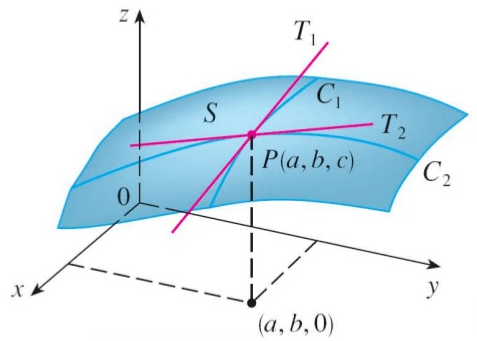
\includegraphics[scale=0.4]{PartialInterpretations.png}
\caption{Geometric Partial Derivatives}
\label{partderiv}
\end{center}
\end{figure}
A surface $S$ is defined by $z = f(x,y)$, where a point $P(a,b,c)$ is present. By setting $y = b$ constant, we focus on the intersection between the plane $y = b$ and $S$, which is the curve $C_1$. Now by taking the derivative respect to $x$ here, you're locating the tangent $T_1$, where the slope of that tangent is $f_x(a,b)$. The same works for $f_y(a,b)$ on $C_2$ and $T_2$.
\subsubsection{Functions of 3+ variables}
To define partials with functions of 3+ variables, just keep 2+ constant and take with respect to one of them.
\begin{gather*}
    f_x(x,y,z) = \lim_{h \to 0} \frac{f(x+h,y,z) - f(x,y,z)}{h}
\end{gather*}
Geometric interpretation here is difficult. Partial derivatives can be taken with functions of any number of variables.
\subsubsection{Higher Order Derivatives}
If $f$ is a function of two variables, then the partial derivatives will also be functions of two variables. This means you can take $f_{xx}$ or $f_{yy}$. You can also take things like:
\begin{gather*}
    f_{xy} = \frac{\p}{\p y}\bigg(\frac{\p f}{\p x}\bigg) = \frac{\p^2f}{\p y \p x}
\end{gather*}
Note that this notation can sometimes be a little confusing, since $f_{xy} = \frac{\p^2f}{\p y \p x}$. So when you see the Leibniz notation, evaluate the rightmost partial first and then the one on the left.

An interesting relationship here is that for most functions, $f_{xy} = f{yx}$, which is called \textbf{Clairaut's Theorem}. It works only when both second order partials are continuous on a "small enough disk" that contains the point.
\begin{proof}
You can prove this by using the limit definiton and you will find that taking the limit of the limit(second derivative) will yield the same number either way(and this will only work when continuous).
\end{proof}

You can also define 3rd order partials similar to how you would define them for normal derivatives.
\subsubsection{Partial Differential Equations}
Partial derivatives occur often in physics as \textbf{partial differential equations} to express physical laws. For example,
\begin{gather*}
    \frac{\p^2 u}{\p x^2} + \frac{\p^2 u}{\p y^2} = 0
\end{gather*}
is called \textbf{Laplace's Equation} and functions that satisfy this are called \textbf{harmonic functions}, which have applications in many physical fields.

The basic \textbf{wave equation}:
\begin{gather*}
    \frac{\p^2 u}{\p t^2} = a^2 \frac{\p^2 u}{\p x^2}
\end{gather*}

This describes the motion of a wave where $u(x,t)$ is the (vertical) displacement of a string from equilibrium. This says that the acceleration of the string's distance from equilibrium is proportional to the acceleration in the string's height with respect to the distance(2nd derivative). For example, functions like $sin(x - at)$ would satisfy this.

\subsection{Tangent Planes and Linear Approximations}
If you zoom in far enough to a single variable function, you will get something that starts to look more and more like a line, the tangent line. This idea should be similar in 3D, instead having a differential that works with two-variable functions instead.
\subsubsection{Tangent Planes}
Let's say a surface $S$ has an equation $z = f(x,y)$, and let $P_0(x_0,y_0,z_0)$ be a point on $S$. Using the direction curves from last section, the \textbf{tangent plane} of $S$ at $P_0$ is defined to be the plane that contains the intersecting tangents which are the slopes of the partial derivatives.
\begin{figure}[H]
\begin{center}
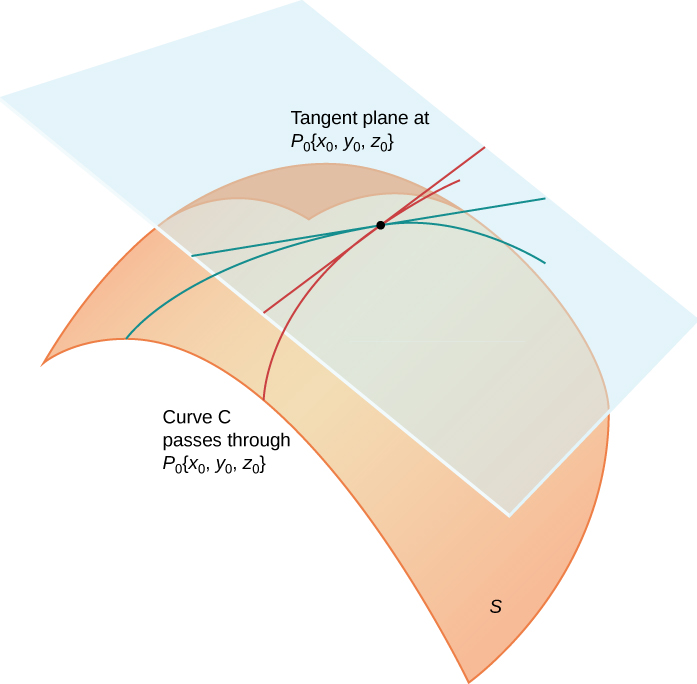
\includegraphics[scale=0.7]{TangentPlanes.jpeg}
\caption{Tangent Plane}
\label{tanplanes}
\end{center}
\end{figure}
The general equation for a plane is:
\begin{gather*}
    A(x-x_0) + B(y-y_0) + C(z-z_0) = 0
\end{gather*}
Dividing by $C$, and letting $a = -\frac{A}{C}$, and $b = -\frac{B}{C}$:
\begin{gather*}
    z - z_0 = a(x-x_0) + b(y-y_0)
\end{gather*}
Now by intersecting it with the plane $y = y_0$:
\begin{gather*}
    z - z_0 = a(x-x_0) \hspace{50pt} y = y_0
\end{gather*}
Notice how this looks similar to point-slope form, wherre $a$ is the slope, which we know to be $f_x(x_0,y_0)$. Doing the same for $y$ we can get:
\begin{gather*}
    z - z_0 = f_x(x_0,y_0) (x-x_0) + f_y(x_0,y_0) (y-y_0)
\end{gather*}
As you zoom in further to $P_0$, the level curves of the function begin to look more and more like parallel lines(with the same slope as a tangent plane), which is similar to the single variable equivalent.
\subsubsection{Linear Approximations}
Note how a tangent plane is similar to a tangent line. In fact, using the tangent plane equation can be a good approximation for the function, but only near the point of approximation and not further. The function $L$ of the tangent plane to a point is called the \textbf{linearization} of $f$ at the point.
\subsubsection{Differentiability}
Sometimes the partial derivatives of a function can exist, so the "differentiability implies continuity" doesn't really work for partial derivatives. Consider $f(x,y)$ with small changes to it:
\begin{gather*}
    \Delta z = f(a + \Delta x, b + \Delta y) - f(a,b)
\end{gather*}
So you can define real differentiability to be when $\Delta z$ can be expressed as:
\begin{gather*}
    \Delta z = f_x(a,b)\Delta x + f_y(a,b) \Delta y + \varepsilon_1 x + \varepsilon_2 y
\end{gather*}
Where both $\varepsilon \to 0$ as $\Delta x, \Delta y \to 0$.

That definition is pretty hard to use so you can see if $f_x$ and $f_y$ exist near $(a,b)$ and are both continuous at that point, then $f$ is differentiable(can you see why?)
\subsubsection{Differentials}
In single-variable calculus, a differential is a small number $dx$ that can be given any small value. The other differential $dy$ is defined as:
\begin{gather*}
    dy = f'(x) dx
\end{gather*}
Now the \textbf{total differential} $dz$ can be defined as adding up all the changes coming from the other differentials, using partial derivatives:
\begin{gather*}
    dz = \frac{\p z}{\p x}dx + \frac{\p z}{\p y}dy
\end{gather*}
So instead using $dx = \Delta x = x - a$ and $dy = \Delta y = y - b$, we can write this in a familiar form:
\begin{gather*}
    dz = f_x(a,b)(x-a) + f_y(a,b)(y-b)
\end{gather*}
This is similar to a linear approximation, in fact we can rewrite the entrie linear approximation as:
\begin{gather*}
    f(x,y) \approx f(a,b) + dz
\end{gather*}
To see the geometric interpretation, $\Delta z$ is the change in the height of the surface, while $dz$ is the change in the height of the \textit{tangent plane}.
\subsubsection{Functions of 3+ Variables}
Extending again to three variables, the \textbf{linear approximation} is:
\begin{gather*}
    f(x,y,z) \approx f(a,b,c) + f_x(a,b,c)(x-a) + f_y(a,b,c)(y-b) + f_x(a,b,c)(z-c)
\end{gather*}
The \textbf{differential}, this time called $dw$:
\begin{gather*}
    dw = \frac{\p w}{\p x}dx + \frac{\p w}{\p y}dy + \frac{\p w}{\p z}dz
\end{gather*}
\subsection{The Chain Rule}
For single variable calculus, the chain rule was:
\begin{gather*}
    \frac{dy}{dt} = \frac{dy}{dx}\frac{dx}{dt}
\end{gather*}
The new chain rule has a few different versions for its different cases.
\subsubsection{Chain Rule One}
\begin{gather*}
    \frac{dz}{dt} = \frac{\p f}{\p x}\frac{dx}{dt} + \frac{\p f}{\p y}\frac{dy}{dt}
\end{gather*}
\begin{proof}
Dividing the definition in the last section by $\Delta t$ yields:
\begin{gather*}
    \frac{\Delta z}{\Delta t} = \frac{\p f}{\p x}\Delta x + \frac{\p f}{\p y} \Delta y + \frac{\varepsilon_1 \Delta x}{\Delta t} + \frac{\varepsilon_2 \Delta y}{\Delta t}
\end{gather*}
Now taking $t \to 0$:
\begin{gather*}
    \frac{dz}{dt} = \frac{\p f}{\p x}\frac{dz}{dt} + \frac{\p f}{\p y} \frac{dy}{dt} + \lim_{t \to 0} \varepsilon_1 \frac{dx}{dt} + \lim_{t \to 0} \varepsilon_2 \frac{dy}{dt}
\end{gather*}
Since both $\varepsilon \to 0$, the final form is proved.
\end{proof}
This theorem should make a lot of sense.
\subsubsection{Chain Rule Two}
This case is used for when $x$ and $y$ are functions of two \textbf{independent variables} $s$ and $t$. By holding one of them constant, you can calculate the partial with respect to the other one by using Chain Rule One.

\begin{gather*}
    \frac{\p z}{\p s} = \frac{\p z}{\p x}\frac{\p x}{\p s} + \frac{\p z}{\p y}\frac{\p y}{\p s}
\end{gather*}
Then do the same thing for the $t$ variable. This should also make sense since you're adding up all the partial changes to get the full change.
\subsubsection{Chain Rule General}
The general chain rule now extends to $n$ variables, and takes on the same form:
\begin{gather*}
    \frac{\p u}{\p t_i} = \frac{\p u}{\p x_1}\frac{\p x_1}{\p t_1} + \frac{\p u}{\p x_2}\frac{\p x_2}{\p t_2}...\frac{\p u}{\p x_n}\frac{\p x_n}{\p t_i}
\end{gather*}
\subsubsection{Implicit Differentiation}
If there's a function of two variables that is defined implicitly: $F(x,y) = 0$. You can differentiate both sides(assume $y = f(x)$):
\begin{gather*}
    \frac{\p F}{\p x}\frac{dx}{dx} + \frac{\p F}{\p y}\frac{dy}{dx}
\end{gather*}
Solving for the derivative:
\begin{gather*}
    \frac{dy}{dx} = -\frac{\frac{\p F}{\p x}}{\frac{\p F}{\p y}} = -\frac{F_x}{F_y}
\end{gather*}
The \textbf{Implicit Function Theorem} from advanced calculus can back this up, showing with certain assumptions that $y$ is a function of $x$ and that this definition holds.

Now if $z = f(x,y)$ and $z$ is a third input variable into a 3 variable function, $F(x,y,f(x,y)) = 0$, then we can write:
\begin{gather*}
    \frac{\p F}{\p x}\frac{\p x}{\p x} + \frac{\p F}{\p y}\frac{\p y}{\p x} + \frac{\p F}{\p z}\frac{\p z}{\p x} = 0
\end{gather*}
Since $\frac{\p y}{\p x} = 0$, we can cancel that term and solve for the other partials:
\begin{gather*}
    \frac{\p z}{\p x} = -\frac{\frac{\p F}{\p x}}{\frac{\p F}{\p z}}\\
    \frac{\p z}{\p y} = -\frac{\frac{\p F}{\p x}}{\frac{\p F}{\p y}}
\end{gather*}
\subsection{Directional Derivatives and the Gradient}
\subsubsection{The Directional Derivative}
Imagining any surface, we know how to find the rate of change going in the $x$ or $y$ directions. However, what if you want to go in \textit{any} direction? Like a direction specified by a point or vector? Enter the \textbf{directional derivative}.

The partial derivatives $f_x$ and $f_y$ already give special cases of the partial derivative in the $\hat{i}$ and $\hat{j}$ directions. But if we want to find the rate of change for $z$ at a point $(x_0,y_0.z_0)$, we can use a general vector $\vv{u} = \vl a,b \vr$. Now consider a random surface $S$.
\begin{figure}[H]
\begin{center}
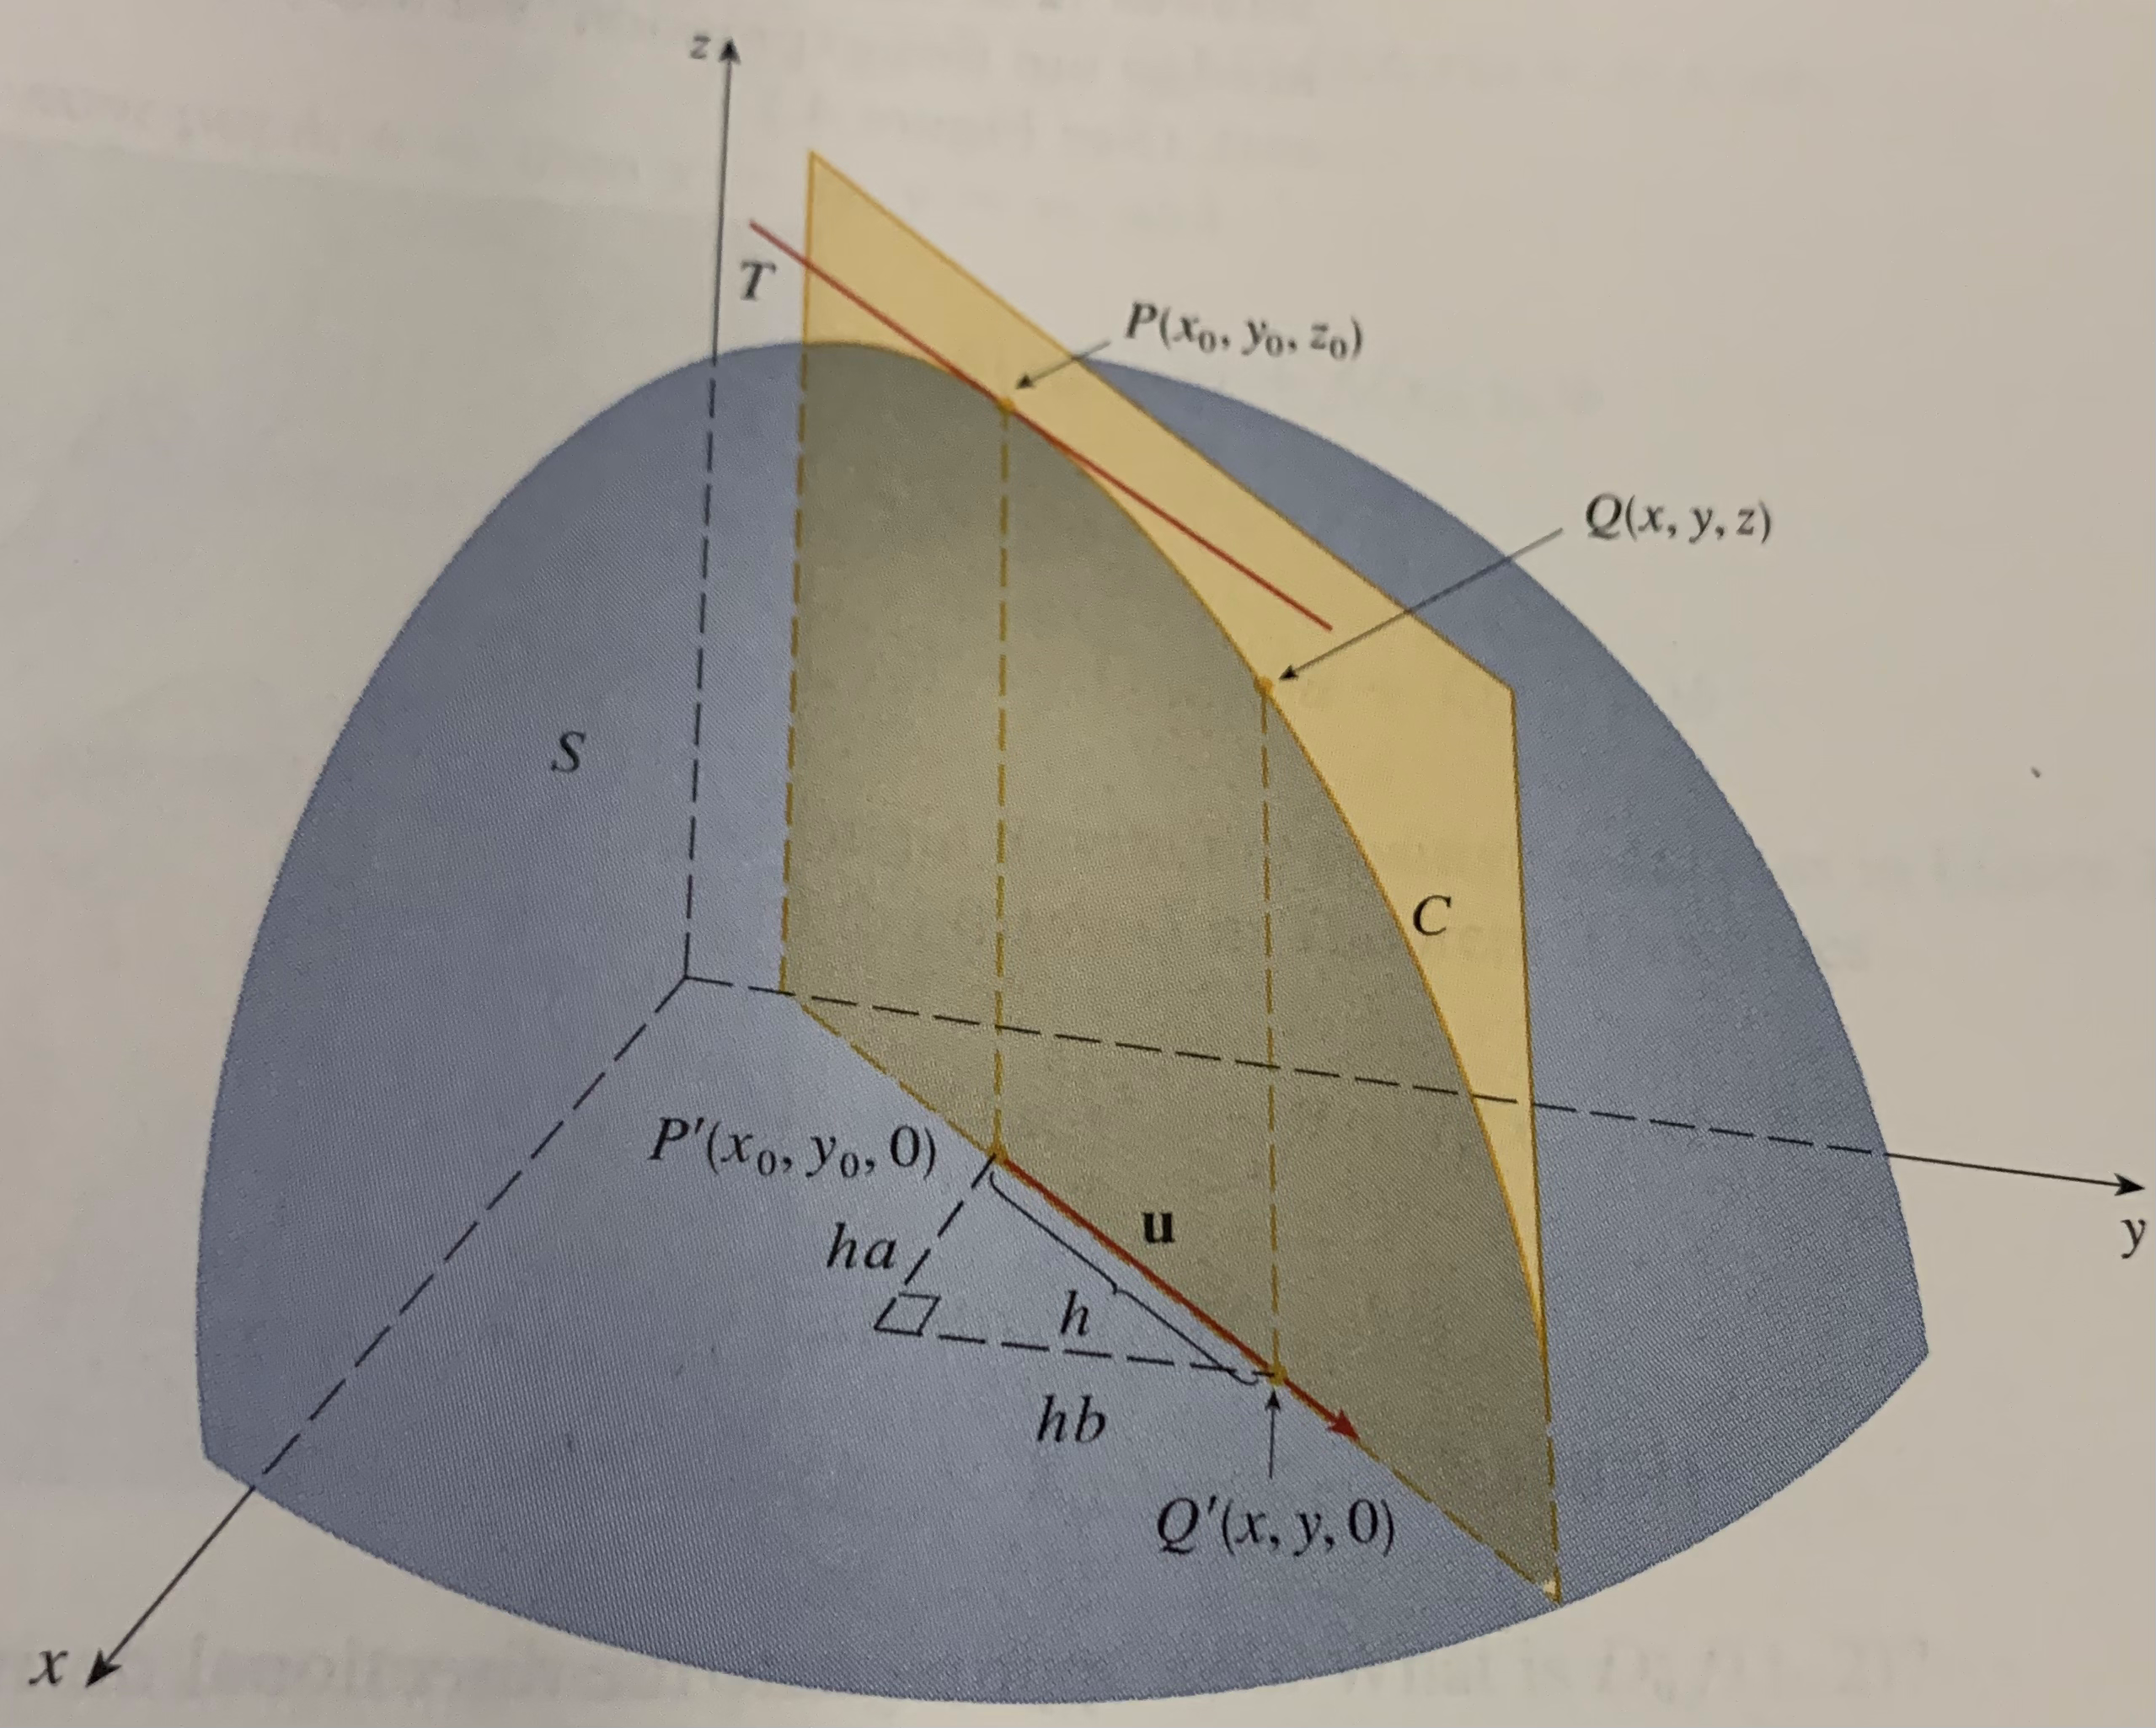
\includegraphics[scale=0.15]{DirectDeriv.png}
\caption{Directional Derivative}
\label{dirderiv}
\end{center}
\end{figure}
The plane that slices through the surface is in the direction of $\vv{u}$ and therefore the tangent $T$ represents the directional derivative in the $\vv{u}$ direction. Imagine a general point $Q(x,y,z)$ on the curve and project both points to $P',Q'$ on the $xy$ plane. Then:
\begin{gather*}
    \vv{P'Q'} = h\vv{u}
\end{gather*}
because $\vv{u}$ is parallel to $\vv{P'Q'}$ since both projected points were on the plane($h$ is a constant here). Looking at the right triangle in Fig. \ref{dirderiv}:
\begin{gather*}
    \Delta x = x - x_0 = ha\\
    \Delta y = y - y_0 = hb\\
    \frac{\Delta z}{h} = \frac{z-z_0}{h} = \frac{f(x_0 + ha, y_0 + hb) - f(x_0,y_0)}{h}
\end{gather*}
Now by taking $h \to 0$, we can find the directional derivative:
\begin{gather*}
    D_{\vv{u}}f(x_0,y_0) = \lim_{h \to 0} \frac{f(x_0 + ha, y_0 + hb) - f(x_0,y_0)}{h}
\end{gather*}
There is often an easier way to apply this, because:
\begin{gather*}
    D_{\vv{u}}f(x,y) = f_x a + f_y b
\end{gather*}
\begin{proof}
Imagine a function of \textbf{single variable} $h$. Remember $h$ is not a constant here, such that:
\begin{gather*}
    g(h) = f(x_0 + ha, y_0 + hb)
\end{gather*}
The normal definition of a derivative gives:
\begin{gather*}
    g'(0) = \lim_{h \to 0}\frac{f(x_0 + ha, y_0 + hb) - f(x_0,y_0)}{h} = D_{\vv{u}}f(x_0,y_0)
\end{gather*}
If we rewrite $g(h) = f(x,y)$, then $x = x_0 + ha$ and $y = y_0 + hb$, now using the Chain Rule:
\begin{gather*}
    g'(h) = \frac{\p f}{\p x}\frac{dx}{dh} + \frac{\p f}{\p y}\frac{dy}{dh} = f_x a + f_y b
\end{gather*}
Now by taking $g'(0)$, we can see that both equations for $g'(0)$ are equal and so QED.
\end{proof}
Note that $\vv{u}$ must be a \textbf{unit vector} for this(pending verification here). Since it is a unit vector, we can use $a = \cos(\theta)$ and $b = \sin(\theta)$ to make $\vv{u} = \vl \cos(\theta), \sin(\theta) \vr$ and you can use an angle to specify the direction instead.
\subsubsection{The Gradient Vector}
Note that from the formula for the directional derivative, you can rewrite it as a dot product of two vectors.
\begin{gather*}
    D_{\vv{u}} f = f_x a + f_y b\\
    = \vl f_x, f_y \vr \vdot \vv{u}
\end{gather*}
The first vector, which consists of the partial derivatives of $f$, is called the \textbf{gradient vector}, or \textbf{grad} $f$, or $\nabla f$, which is read "del" f.n So:
\begin{gather*}
    \nabla f = \frac{\p f}{\p x}\hat{i} + \frac{\p f}{\p y}\hat{j}\\
    D_{\vv{u}} f = \n f \vdot \vv{u}
\end{gather*}
All the concepts discussed in this section so far work for multiple dimensions as well.
\subsubsection{Maximizing the Directional Derivative}
Imagine a differentiable function $f$ of 2-3 variables. The \textbf{maximum value} of the directional derivative is $|\n f(\vv{x})|$ and it occurs when $\vv{u}$ points in the same direction as $\vv{\n f(x)}$.
\begin{proof}
\begin{gather*}
    D_{\vv{u}} f = \n f \vdot \vv{u} = |\n f||\vv{u}| \cos(\theta) =  |\n f| \cos(\theta)
\end{gather*}
The max. value occurs when $\theta = 0$, and it's the magnitude of the gradient vector. When $\theta = 0$, that means $\vv{u}$ and $\n f$ are in the same direction.
\end{proof}
\subsubsection{Tangent Planes to Level Surfaces}
Imagine a level surface with $F(x,y,z) = k$ with $P(x_0,y_0,z_0)$. Define a curve $C$ that lies on the surface, so the curve can be detailed by $\vv{r}(t) = \vl x(t), y(t), z(t) \vr$, where P is a point on that. If $F$ and $x,y,z$ are differentiable:
\begin{gather*}
    \frac{\p F}{\p x}\frac{dx}{dt} + \frac{\p F}{\p y}\frac{dy}{dt} + \frac{\p F}{\p z}\frac{dz}{dt} = 0
\end{gather*}
Synthesizing this with a dot product:
\begin{gather*}
    \n F \vdot \vv{r}'(t) = 0
\end{gather*}
Particularly, $\n F(x_0,y_0,z_0) \vdot \vv{r}'(t_0) = 0$. Notice how this equation looks very similar to a plane. This equation means that the gradient is always perpendicular to the tangent vector to any curve that passes through the point on the surface. So now we can define the \textbf{tangent plane} to be the plane with normal vector $\n F$ that passes through the point $P$. Rewriting tihs:
\begin{gather*}
    F_x(x - x_0) + F_Y(y-y_0) + F_z(z-z_0) = 0
\end{gather*}
Converting this to the symmetric form:
\begin{gather*}
    \frac{x-x_0}{F_x} = \frac{y - y_0}{F_y} = \frac{z - z_0}{F_z}
\end{gather*}
Remember that we talked about tangent planes before, for the special case when it's only $z = f(x,y)$. You can write $F(x,y,z) = f(x,y) - z = 0$. Since you know $F = 0$ always, you can write the partial derivatives:
\begin{gather*}
    F_x = f_x\hspace{20pt}F_y = f_y \hspace{20pt}F_z = -1
\end{gather*}
So this special case becomes:
\begin{gather*}
    f_x(x-x0) + f_y(y-y_0) -(z-z_0) = 0
\end{gather*}
Rearranging this will get the tangent plane equation we found in section 15.4.
\subsubsection{Significance of the Gradient}
The gradient vector will always point in the direction of the \textbf{fastest increase}, we also know that the gradient will also point in the perpendicular direction to the level surface. Along the level surface, $f$ stays constant, so traveling $\perp$ to that will give you the fastest increase(think equipotential lines in a way). The gradient vector from a point can map out a curve that draws the curve of fastest ascent of $f$.
\subsection{Maximum and Minimum Values}
One of the most useful applications of the normal derivative was to find maximum and minimum values. $f(a,b)$ is a local maximum if for all points $(x,y)$ on a disk near $(a,b)$, $f(a,b) \geq f(x,y)$ and less for a local minimum. If these work for all points in the domain then they are absolute maxima or minima.

If $f(a,b)$ is a local maximum or minimum at a point and the partial derivatives exist, then both partial derivatives must be zero at that point.
\begin{proof}
The reason this makes sense is because if you take a slice in the x or y directions, the same first derivative test should work as well(intuition there).
\end{proof}
If you think about it, whenever you have a local max or min, the tangent plane should be tangent. A point is a \textbf{critical point} if $f_x$ and $f_y$ both $= 0$. Now if you remember from single variable calculus, not all critical points are maxima or minima. Some are neither.

This is actually possible in 3D. You can have a tangent plane be horizontal and not be a local min or max.
\begin{figure}[H]
\begin{center}
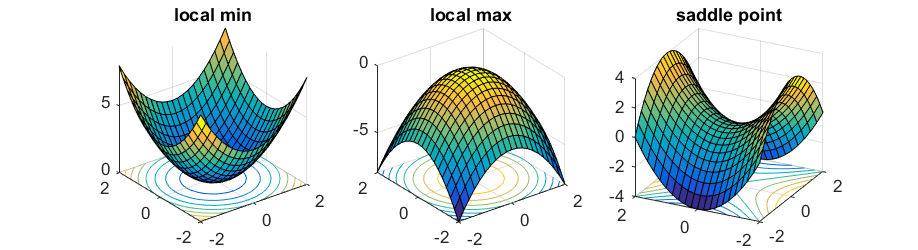
\includegraphics[scale=0.7]{saddlePoint.png}
\caption{Saddle Point}
\label{saddle}
\end{center}
\end{figure}
It's not a local maximum or minimum, but the tangent at the center is horizontal. This is called a \textbf{saddle point}. There's also something similar to the \textit{second derivative test} in single variable calculus.

If the second partial derivatives of $f$ are continuous on a disk around $(a,b)$, where $f_x = 0$ and $f_y = 0$ there. Basically, $(a,b)$ is a critical point. Let:
\begin{gather*}
    D = D(a,b) = f_{xx}(a,b)f_{yy}(a,b) - \bigg[f_{xy}(a,b)]\bigg]^2
\end{gather*}
\begin{enumerate}
    \item If $D > 0$ and $f_{xx}(a,b) > 0$, then $f(a,b)$ is a local max.
    \item If $D > 0$ and $f_{xx}(a,b) < 0$, then $f(a,b)$ is a local min.
    \item If $D < 0$, then this point is neither, it is a \textbf{saddle point}.
\end{enumerate}
This form can be written as a determinant:
\begin{gather*}
\begin{bmatrix}
f_{xx} & f_{xy}\\
f_{yx} & f_{yy}
\end{bmatrix}
\end{gather*}
Notice how this form works and is easy to remember.
\begin{proof}
The first order directional derivative on $\vv{u} = \vl h,k \vr$ is:
\begin{gather*}
    D_{\hat{u}} f = f_x h + f_y k
\end{gather*}
Take the directional derivative a second time and complete the square(it's actually pretty complicated to do).
\end{proof}
\subsubsection{Absolute Maxima and Minima}
For a function of one variable continuous on $[a,b]$, $f$ must attain a maximum and a minimum value by the extreme value theorem. This can be similar for two variable functions as well. However, to define an interval here we need to use a disk. A \textbf{closed set} contains the disk as well as the circle bounding it while an \textbf{open set} does not. A \textbf{bounded set} is a set which is contained within one disk. Within a closed, bounded set, a continous function $f$ must attain a maximum and minimum value at some point within it. To find these values:
\begin{enumerate}
    \item Find the values of $f$ which are critical points.
    \item Find the max and min values on the boundary of the interval(set).
    \item Compare those values to find the absolute max and min
\end{enumerate}
\subsection{Lagrange Multipliers}
Lagrange's Method makes it possible to find the maximum and minimum values of a function $f$ of 2+ variables when there is a constraint(s) $g(x,y) = k$ or $g(x.y,z) = k$.
\begin{figure}[H]
\begin{center}
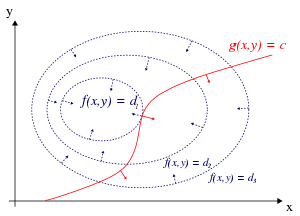
\includegraphics[scale=0.7]{LagrangeMultiplier.png}
\caption{Level Curve Intersections}
\label{lag-mult}
\end{center}
\end{figure}
We want to find any extreme values of $f$ when $f(x,y)$ lies on the level curve $g(x,y) = k$. This maximum value happens at the largest level curve of $f$(level curves in red) where they just barely meet. This largest value will have share the tangent with $g$. This works because remember $f$ has infinitely many level surfaces, so the highest one does exist and does share the tangent. Since both $\n f$ and $\n g$ are perpendicular to their tangents, a shared tangent means the gradient vectors are parallel.

Since they are parallel, there must be a number $\lambda$ such that:
\begin{gather*}
    \n f(x_0,y_0,z_0) = \lambda \n g(x_0,y_0,z_0)
\end{gather*}
This number is called the \textbf{Lagrange Multiplier}.

So to find the max and min values, first solve the system of equations for all $(x,y,z)$ such that:
\begin{gather*}
    \n f(x,y,z) = \lambda \n g(x,y,z)\hspace{20pt}g(x,y,z) = k
\end{gather*}
The compare these points to find the min. and max. values of $f$. If you write the equations in terms of scalar components:
\begin{gather*}
    f_x = \lambda g_x\hspace{20pt}f_y = \lambda g_y\hspace{10pt}...\hspace{10pt}g(x,y,z) = k
\end{gather*}
\subsubsection{Two Constraints}
When using 4D functions, you can add two constraints. When you imagine the level surfaces of such a function, they would be normal 3D surfaces. This means that you could intersect them to form a curve $C$. The gradients to both surfaces would be orthogonal to C, and so they themselves are perpendicular(assuming they aren't parallel). You can write(similar to $\hat{i}$ and $\hat{j}$ vector notation):
\begin{gather*}
    \n f = \lambda \n g + \mu \n h
\end{gather*}
By using components, which are the partials in each direction, you can effectively solve a system of equations that would find all the points, and compare those to find the max and min.
\section{Multiple Integrals}
\subsection{Double Integrals Over Rectangles}
The single integral was used to solve the problem of area under a curve, so a \textbf{double integral} could possibly be used to find the volume under a surface by taking the integral of the integral.
\subsubsection{Single Integrals}
Recall that:
\begin{gather*}
    \int_a^b f(x) dx = \lim_{n \to \infty} \sum_{i = 1}^n  f(x_i) \Delta x
\end{gather*}
Where that integral represents the area under $f(x)$ from $a$ to $b$.
\subsubsection{Double Integrals and Volume}
We can start by defining $f(x,y)$ defined on a closed rectangle $a \leqslant x \leqslant b$ and $c \leqslant y \leqslant d$.
\begin{figure}[H]
\begin{center}
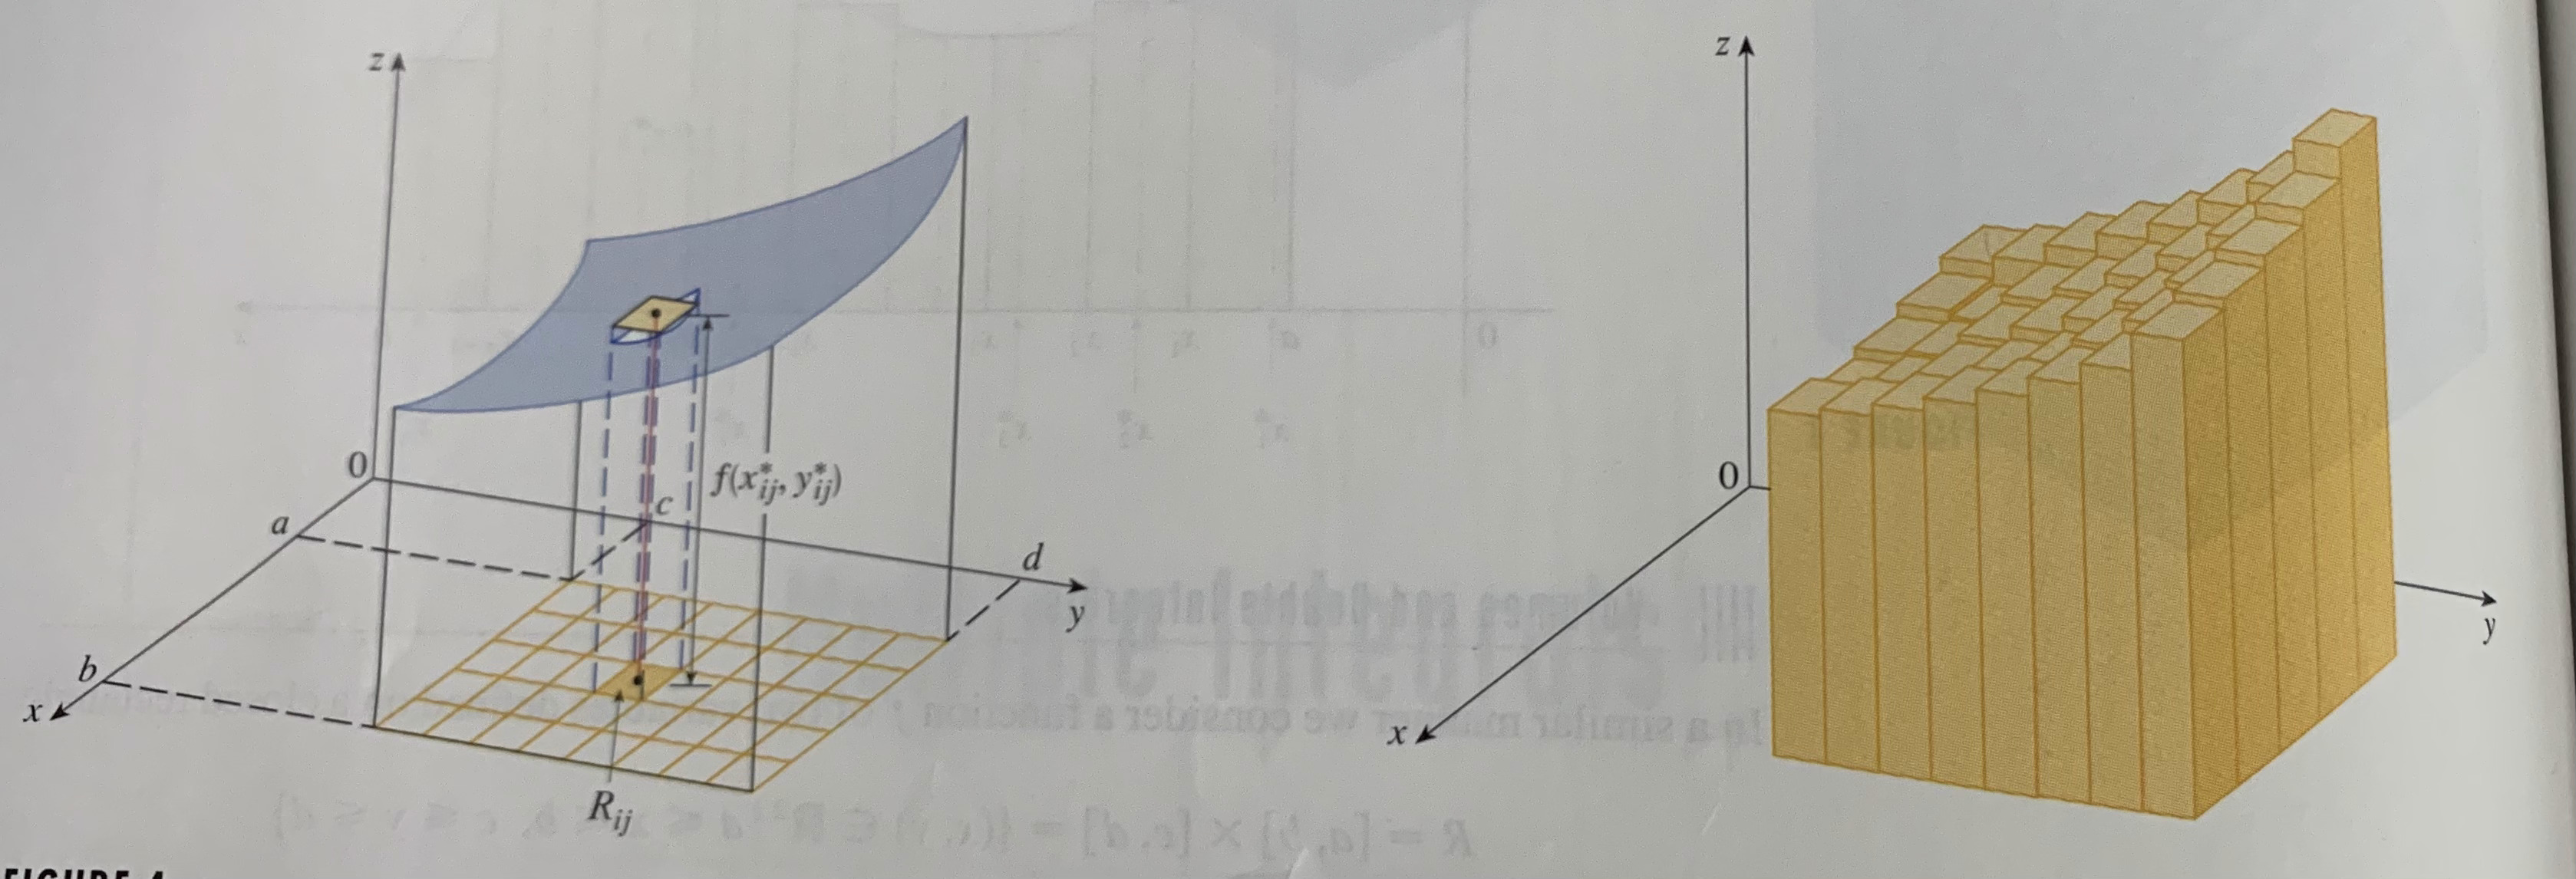
\includegraphics[scale=0.15]{doubleint.jpg}
\caption{Approximating Double Integrals}
\label{doubleint}
\end{center}
\end{figure}
Split the area on the $xy$ plane into a bunch of smaller squares to approximate. Each square has area $\Delta A = \Delta x \Delta y$. If we choose some sample point $(x_i*,y_i*)$ on each square, the volume of each box is given by:
\begin{gather*}
    V_{ij} = f(x_i*,y_i*) \Delta A
\end{gather*}
To add all these boxes up:
\begin{gather*}
    V \approx \sum_{i = 1}^m\sum_{j = 1}^n f(x_{ij}*,y_{ij}*) \Delta A
\end{gather*}
As $m$ and $n$ get larger, the approximation will get better, so to find our final volume we need to take the limit.
\begin{gather*}
    V = \lim_{m,n \to \infty}\sum_{i = 1}^m\sum_{j = 1}^n f(x_{ij}*,y_{ij}*) \Delta A
\end{gather*}
So we can define the double integral over a rectangle $R$ as:
\begin{gather*}
    \iint_R f(x,y) dA = \lim_{m,n \to \infty}\sum_{i = 1}^m\sum_{j = 1}^n f(x_{ij}*,y_{ij}*) \Delta A
\end{gather*}
If $f(x,y) \geqslant 0$, then you can define the volume below $z = f(x,y)$:
\begin{gather*}
    V = \iint_R f(x,y)
\end{gather*}
\subsubsection{The Midpoint Rule}
All the integral approximation methods for single integrals all have counterparts for double integrals. For example, the midpoint rule here uses a double Reimannn sum with points $(x_i,y_j)$ that are in the center of the boxes. These points are $\bar{x_i} = x_i - x_{i-1}$ and similarly for $y$.
Therefore, we can define the midpoint rule:
\begin{gather*}
    \iint_R f(x,y) dA = \lim_{m,n \to \infty}\sum_{i = 1}^m\sum_{j = 1}^n f(\bar{x_{i}},\bar{y_{i}}) \Delta A
\end{gather*}
\subsubsection{Average Value}
Remember that the average value of a single variable function was:
\begin{gather*}
    Average = \frac{1}{b - a}\int_a^b f(x) dx
\end{gather*}
Think about why this works. Area is base times height, and so taking the area and dividing by the base($b-a$) should give you the average height.

So similarly, average value can be shown as:
\begin{gather*}
    Average = \frac{1}{A(R)}\iint_R f(x,y) dA
\end{gather*}
where $A(R)$ is the area of the region $R$. If you have $f \geqslant 0$, you can say that:
\begin{gather*}
    A(R) \times Average = \iint_R f(x,y) dA
\end{gather*}
This says that the square area of the region times the average height has the same volume as the volume under the surface.
\subsubsection{Properties of Double Integrals}
Most of the same properties in single integrals apply to double as well, since both are composed of similar sums. For example, addition of integrals(called \textit{linearity}) holds too. Multiplying a constant $c$ by an integral can be removed from the integral, etc.
\subsection{Iterated Integrals}
Imagine a function $f(x,y)$ that is continuous on a rectangle $R = [a,b] \times [c,d]$. So $\int_c^d f(x,y) \d y$ means that $x$ is held constant while the integral is carried out, which is called \textbf{partial integration}. Note how this is similar to a partial derivative. Since the actual value of the integral depends on $x$, we can write:
\begin{gather*}
    A(x) = \int_c^d f(x,y) dy
\end{gather*}
Now if we integrate once more we get:
\begin{gather*}
    \int_a^b \int_c^d f(x,y) \,dy \,dx
\end{gather*}
When you integrate this, you always start from the inside and work your way out(similar to the Leibniz notation on partial derivatives).

Now you can probably see where this is going. According to \textbf{Fubini's Theorem}, if $f(x,y)$ is continuous on $R$ then:
\begin{gather*}
    \iint_R f(x,y) \,dA = \int_a^b \int_c^d f(x,y) \,dy\,dx = \int_c^d \int_a^b f(x,y) \,dx\,dy
\end{gather*}
The actual proof for this is a little difficult, but if you think about integrating a solid, holding one variable constant gives you the area of a \textit{slice} of the solid. Now integrating the other variable will add up those area slices and give you the solid(which is the volume or the double integral). This should work both ways if you think about it.
\subsection{Double Integrals Over General Regions}
When integrating with a single integral, you always need to integrate over an interval(i.e $[0,2$). But with a double integral you need to integrate over a region which may or may not be a rectangle. But is that really true? With $f(x,y)$, define a new function $F$ which is $f(x,y)$ when you're in $R$ but $0$ if you're outside of it. $F$ should be defined on a rectangle so you can integrate. Since the parts outside $R$ do not contribute to the integral, they don't change the answer.
\subsubsection{Type I and II Regions}
A region is \textbf{Type I} if it lies between the graphs of two continuous functions of $x$, for example:
\begin{gather*}
    D = {(x,y) | a \leqslant x \leqslant b, g_1(x) \leqslant y \leqslant g_2(x)}
\end{gather*}
This means the region is bounded by 2 continuous functions and two lines $x=a$ and $x=b$. But how does this help integration?
\begin{figure}[H]
\begin{center}
\includegraphics[scale=0.5]{genregions.png}
\caption{Type I and II Regions}
\label{genregions}
\end{center}
\end{figure}
So to integrate:
\begin{gather*}
    \iint_R f(x,y) \,dA = \int_a^b\int_c^d f(x,y) \,dA = \int_a^b\int_{g_1(x)}^{g_2(x)} f(x,y) \,dA
\end{gather*}
Notice why this works. To the $y$ variable, both functions of $x$ are essentially constants. Remember integration is just addition, so you take each piece of $y$ that has it's own $g$-values, and add them together.

A \textbf{Type II} region is similar except that the functions are of $y$ and not $x$.
\textbf{Important}: Make sure you always draw a diagram or visualize what you are integrating. If you don't, you risk making mistakes.
\subsubsection{Properties of Double Integrals}
Two properties of double integrals we already know from 16.1. The \textbf{linearity}, an integral of a sum is the sum of the integrals, and you can pull a constant out of an integral. This one should also make sense. When $f \geqslant g$:
\begin{gather*}
    \iint_D f(x,y) \,dA \geqslant \iint_D g(x,y) \,dA
\end{gather*}
Now imagine the region $D$. If you split that region into two $D_1$ and $D_2$ that together can form $D$:
\begin{gather*}
    \iint_D f(x,y) \,dA = \iint_{D_1} f(x,y) \,dA + \iint_{D_2} f(x,y) \,dA
\end{gather*}
Another property:
\begin{gather*}
    \iint_D 1 \,dA = Area(D)
\end{gather*}
This should make sense. Think about a box. If the height of the box is $1$, then the volume of the box is numerically the same as the area of the box.

So by making use of the last few properties, given that $m \leqslant f(x,y) \leqslant M$:
\begin{gather*}
    m\times A(D) = \iint_D f(x,y) \,dA \leqslant M\times A(D)
\end{gather*}
This is a little confusing, but you can get this simply by integrating the given inequality. This is useful though, since it allows you to bound the value of the integral if you can bound the value of $f$.
\subsection{Double Integrals in Polar Coordinates}
Why do we use polar coordinates? Some regions are easier to describe using them. So if we want to evaluate a double integral over a circle, or a region bounded by circles, polar coordinates could come in handy.

Remember from Ch. 11 that these conversions apply:
\begin{gather*}
    r = x^2 + y^2 \hspace{20pt} x = r\cos(\theta) \hspace{20pt} y = r\sin(\theta)
\end{gather*}
So now we can define a \textbf{polar rectangle}, where the dimensions are the polar dimensions:
\begin{gather*}
    R =\{(r,\theta)\,|\, a \leqslant r \leqslant b,\, \alpha \leqslant \theta \leqslant \beta\}
\end{gather*}
\begin{figure}[H]
\begin{center}
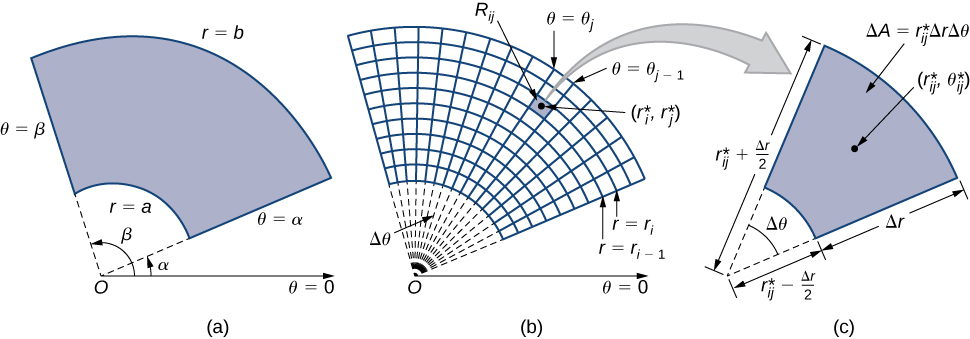
\includegraphics[scale=0.5]{PolarRect.png}
\caption{Polar Integration}
\label{polrect}
\end{center}
\end{figure}
We can split this rectangle into small sections too, into $m$ subsections where $\Delta r = \frac{b-a}{m}$ and $\Delta \theta = \frac{\beta - \alpha}{m}$. So the circles $r = r_i$ and outward lines $\theta = \theta_j$ split the big rectangle into many smaller ones.

The center of one of the subrectangles has polar coordinates:
\begin{gather*}
    r_i^* = \frac{1}{2}(r_{i-1} + r_i)\hspace{20pt}\theta_j^* = \frac{1}{2}(\theta_{j-1} + \theta_j)
\end{gather*}
Now we can find the area of the subrectangle by subtracting circles $r = b$ and $r = a$ over $\Delta \theta = \theta_j - \theta_{j-1}$:
\begin{gather*}
    \Delta A_i = \frac{1}{2}(r_i^2 - r_{i-1}^2) \,\Delta \theta = \frac{1}{2}(r_i + r_{i-1})(r_i - r_{i-1}) \,\Delta \theta = r_i^* \Delta r \Delta \theta
\end{gather*}
So using this we can write a Reimann sum, where $f(x,y)$ now becomes $f(r_i^* \cos(\theta_j^*), r_i^* \sin(\theta_j^*))$. So if we write $g(r,\theta) = r * f(r\cos(\theta),r\sin(\theta))$ then we can get:
\begin{gather*}
    \sum_{i=1}^m\sum_{j=1}^n g(r_i^*,\theta_j^*) \Delta r \Delta \theta = \int_\alpha^\beta \int_a^b g(r,\theta) \,dr \,d\theta = \int_\alpha^\beta \int_a^b f(r \cos(\theta), r \sin(\theta))\,r\,dr\,d\theta
\end{gather*}
\textbf{Important:} Notice the leftover $r$ factor. This is because in a polar rectangle $dA = r\,dr\,d\theta$. Think about why this is. The total circumference of a circle is $\theta r$, where $\theta = 2\pi$. So the small circumference element will be $r \, d\theta$. A rectangle has $A = bh$, where $b = r \, d\theta$ and $h = dr$. So it makes sense that $dA = r\,dr\,d\theta$. Sidenote, make sure that you use the correct limits on the integral when using this formula.
\subsubsection{General Regions}
We can imagine a random polar region bounded by $r = h_2(\theta)$ and $r = h_1(\theta)$. So if the surface function $f$ is continuous on the region then:
\begin{gather*}
    \iint_R f(x,y) \, dA = \int_\alpha^\beta \int_{h_1(\theta)}^{h_2(\theta)} f(r \cos(\theta), r \sin(\theta))\,r\,dr\,d\theta
\end{gather*}
Notice how if you use $f(x,y) = 1$, you can get $\int \frac{1}{2} r^2(\theta) \, d\theta$, which we know is correct since $\iint_R \, dA = A$.
\subsection{Applications of Double Integrals}
Double integrals have many useful physical applications such as finding mass, electric charge, center of mass, and moment of inertia.
\subsubsection{Density and Mass}
A \textbf{lamina} is a 2D plate which looks similar to a region. Imagine a lamina as a region $D$ which its \textbf{density} $\rho(x,y)$ is a continuous function where in mass and area:
\begin{gather*}
    \rho(x,y) = \lim_{\textrm{rect} \to 0} \frac{\Delta m}{\Delta A}
\end{gather*}
This is where the dimensions of a small rectangle enclosing $(x,y)$ approach $0$. If we divide up the lamina into many smaller rectangles, we can find the total mass using the density. For a constant density, remember that $m = \rho A$, so we can use a similar integral form:
\begin{gather*}
    m = \iint_D \rho(x,y) \, dA
\end{gather*}
This idea works for any type of density. For example the \textbf{charge density} $\sigma$ can be used to find total charge on an area.
\begin{gather*}
    Q = \iint_D \sigma(x,y)\, dA
\end{gather*}
\subsubsection{Moments and Centers of Mass}
The \textbf{moment} of a particle on an axis is the product of its mass and distance from the axis. We can find the moment of the entire thing by adding up the particle moments. So we know that for density $m = \rho \Delta A$, so we can write for each particle:
\begin{gather*}
    M_x = (\rho(x,y) \Delta A)y \implies \iint_R y\rho(x,y)\,dA
\end{gather*}
If we're going around the $x$-axis. If we use the $y$-axis then we can use $x$ in the integral instead. This should make sense, since $y$ is the distance from the $x$-axis to the edge of the thing.

The \textbf{center of mass} is a point where we can treat all the mass of something concentrated there. This basically is the weighted "average" point for the mass of the entire thing. In other words, for the $y$-moment: $M_y = m\bar{x}$. The bar just means center fo mass point. Therefore:
\begin{gather*}
    \bar{x} = \frac{1}{m}\iint_R x\rho(x,y) \, dA\\
    m = \iint_R \rho(x,y) \, dA
\end{gather*}
So to find center of mass you may need to solve two double integrals.
\subsubsection{Moments of Inertia}
The \textbf{moment of inertia}(not to be confused with the other moment) of any particle about an axis is $mr^2$, where $m$ is the mass and $r$ is the distance from the axis. So we can find the moment of inertia of a lamina by using a similar method as the last section.
\begin{gather*}
    I_x = \iint_R y^2 \rho(x,y) \,dA
\end{gather*}
It is also useful to find the moment of inertia \textbf{about the origin}, which is also called the \textbf{polar moment of inertia}:
\begin{gather*}
    I_0 = \iint_R (x^2+y^2) \rho(x,y) \, dA
\end{gather*}
Notice how $I_0 = I_x + I_y$. If you need to solve all three, don't be an idiot and actually do all three double integrals.

In general, the moment of inertia is the analog of mass in rotational motion(i.e. $F = ma$ becomes $\tau = I \alpha$).

The \textbf{radius of gyration} of a lamina around an axis is the number $R$ such that:
\begin{gather*}
    I = mR^2
\end{gather*}
This means that if all the mass of the lamina were pushed to a distance $R$ from the axis, then the moment of inertia would be the same as the current lamina. So around the $x$-axis, we have:
\begin{gather*}
    I_x = m\bb{y}^2
\end{gather*}
Here the double bars represent the radius of gyration. So if all the mass was concentrated at $(\bb{x},\bb{y})$ then the moment of inertia \textit{with respect to the axes} would not change.
\subsubsection{Probability}
The probability density function $f(x)$ for any continuous random variable shows the probability that the variable lies at any particular point. This means that $f(x) \geqslant 0$ and that $\int_{-\infty}^\infty f(x) = 1$, which should make sense since if you add all the probabilities everywhere you should get $1$. But to find the probability that the variable exists between $a$ and $b$, you can just use:
\begin{gather*}
    P = \int_a^b f(x) \, dx
\end{gather*}
If you consider two variables $X$ and $Y$(don't confuse them with the lowercase ones), we can use a \textbf{joint density function} to see the chances that $(X,Y)$ lies in a region $D$.

Because probabilities can never be negative and must total to be 1, we have these properties:
\begin{gather*}
    f(x,y) \geqslant 0 \hspace{20pt} \iint_{\mathbb{R}^2} f(x,y) \, dA = 1
\end{gather*}
Just to note, we define $\mathbb{R}^2$ as the limit of $(-\infty, \infty)$ in any coordinate system(expanding boxes, expanding circles, etc.)

If $X$ is a random variable with probability function $f_1(x)$ and $Y$ another one with $f_2(y)$, then $X$ and $Y$ are \textbf{independent} if:
\begin{gather*}
    f(x,y) = f_1(x) f_2(y)
\end{gather*}
That's how independent variables work normally. What are the odds of flipping heads and it raining outside? Multiply the odds of both happening.

If $\mu$ is the average waiting time, then you can model waiting times by using the exponential decay function:
\begin{gather*}
    f(t) = \left\{
        \begin{array}{ll}
            0 & \quad t < 0 \\
            \mu^{-1}e^{\frac{-t}{\mu}} & \quad t \geq 0
        \end{array}
    \right.
\end{gather*}
\subsubsection{Expected Values}
If $X$ is a random variable, then its \textbf{mean} location is:
\begin{gather*}
    \mu = \int_{-\infty}^\infty xf(x) \, dx
\end{gather*}
This should make sense because $f(x)$ weights each location $x$ based on the probability. We can do a similar thing with a joint probability function:
\begin{gather*}
    \mu_x = \iint_{\mathbb{R}^2} xf(x,y) \, dA \hspace{20pt} \mu_y = \iint_{\mathbb{R}^2} yf(x,y) \, dA
\end{gather*}
Notice how these equations are very similar to the moment ones. You can calculate probability just like you calculate mass, by integrating some density function over a region. The total "mass" is $1$ here. You can think about the $\mu$ values as the center of mass.

Lastly, there are \textbf{normal distributions}, which are true if the density function is:
\begin{gather*}
    f(x) = \frac{1}{\sigma \sqrt{2\pi}}e^\frac{-(x-\mu)^2}{2\sigma^2}
\end{gather*}
\subsection{Surface Area}
We can use double integrals to find out the surface area of a surface bounded by some region on the $xy$-plane. So let $S$ be a surface given by $z = f(x,y)$ and you can approximate a small rectangle on the $xy$-plane and find the corner of the rectangle closest to the origin. Get the tangent plane to that and if you do it for smaller and smaller rectangles, your approximation will get better and better.

The tangent plane has to be some sort of parallelogram(think about it), so it can be defined by two vectors:
\begin{gather*}
    \vv{a} = \Delta x \,\hat{i} + f_x \Delta x \,\hat{j}\\
    \vv{b} = \Delta y \,\hat{i} + f_y \Delta y \,\hat{j}
\end{gather*}
We know the area of a parallelogram here is $|\vv{a} \times \vv{b}|$ and so if you cross them you get:
\begin{gather*}
    |\vv{a} \times \vv{b}| = \sqrt{\bigg(\frac{\p z}{\p x}\bigg)^2 + \bigg(\frac{\p z}{\p y}\bigg)^2 + 1} \, \Delta A
\end{gather*}
So now if we convert it to double integral form:
\begin{gather*}
    A = \iint_D \sqrt{\bigg(\frac{\p z}{\p x}\bigg)^2 + \bigg(\frac{\p z}{\p y}\bigg)^2 + 1} \, dA
\end{gather*}
Notice how this is similar to the arc length formula.
\subsection{Triple Integrals}
Single integrals work for $f(x)$, double integrals work for $f(x,y)$, so were can define \textbf{triple integrals} to work for $f(x,y,z)$. So in this case the "region" used would be a box, where we use the same constraints as double integrals with $r \leqslant z \leqslant s$.

If we divide the big box into smaller sub boxes, we can have each box with $\Delta V = \Delta x \, \Delta y \, \Delta z$. Using the same logic as the double integral:
\begin{gather*}
    \iiint_B f(x,y,z) \, dV = \sum_{i=1}^l\sum_{j=1}^m\sum_{k=1}^n f(x_i,y_j,z_k) \, \Delta V
\end{gather*}
This method is not really used in practice so we can apply Fubini's Theorem here:
\begin{gather*}
    \iiint_B f(x,y,z) \, dV = \int_r^s \int_c^d \int_a^b f(x,y,z) \, dx\, dy\, dz
\end{gather*}
Of course, you can integrate in whatever order is easiest and still get the same answer.
\subsubsection{Triple Integrals on General Regions}
We can do this the same way we did for double integrals, where we define it over a rectangle where the function exists but everything not on the rectangle is $0$, and so does not contribute to the integral.

A solid region is \textbf{type I} if it lies between two continuous $z$-functions(functions of $x,y$). So you would evaluate like so:
\begin{gather*}
    \iiint_E f(x,y,z) \, dV = \iint_D \int_{u_1(x,y)}^{u_2(x,y)} f(x,y,z) \,dz \, dA
\end{gather*}
It is not as easy here though, because the remaining region $D$ can also be bounded by functions, for example a \textbf{type I} plane region, where the 2D region is bounded by two functions of $y$.

Basically, integrate one step at a time and be sure you know exactly which order you are integrating in.

A solid region is \textbf{type II} if it is bounded by two surface $x$ functions, and \textbf{type III} if it is bounded by two $y$ surface functions. Of course, in each case after you pass the first integral, the 2D region $D$ could be either type I or type II. Don't confuse plane and solid regions.
\subsubsection{Applications of Triple Integrals}
Single integrals help find the area, double integrals help find volume, but triple integrals are meaningless there because their functions exist in 4D, and a 4D volume is difficult to visualize. However, triple integrals are useful when you have 3 inputs and 1 output, and still need a way to integrate over that.

First of all, if $f(x,y,z) = 1$, then:
\begin{gather*}
    V = \iiint_E \, dV
\end{gather*}
This should make sense, because you're just adding up the tiny blocks of the box, and then multiplying them by $1$.

Any applications of double integrals can easily be extended to triple, for example mass:
\begin{gather*}
    m = \iiint_E \rho(x,y,z) \, dV
\end{gather*}
This time, the moments will be with respect to the axis which is the intersection of the coordinate planes:
\begin{gather*}
    M_{yz} = \iiint_E x\rho(x,y,z) \, dV
\end{gather*}
To find the moment off of the intersection of any two planes, use the other variable in the integrand. Similarly for center of mass,
\begin{gather*}
    \bar{x} = \frac{M_{yz}}{m}
\end{gather*}
The center of mass is located at $(\bar{x},\bar{y},\bar{z})$. If density of is constant, then this point is called the \textbf{centroid}. The \textbf{moments of inertia} off of the three coordinate axes:
\begin{gather*}
    I_x = \iiint_E (y^2 + z^2) \rho(x,y,z) \, dV
\end{gather*}
and similarly for the rest of the variables.

The total electric charge on a solid object can be found with a triple integral(if the density is a function of three variables):
\begin{gather*}
    Q = \iiint_E \sigma(x,y,z)\, dV
\end{gather*}
If you want probability with three variables $XYZ$ then the \textbf{joint density function} satisfies:
\begin{gather*}
    f(x,y,z) \geqslant 0 \hspace{20pt} \int_{-\infty}^\infty\int_{-\infty}^\infty\int_{-\infty}^\infty f(x,y,z) \,dz \, dy \, dx = 1
\end{gather*}
Particularly, to find the probability that $(X,Y,Z)$ lies in the solid $E$:
\begin{gather*}
    P = \iiint_E f(x,y,z) \,dz\,dy\,dx
\end{gather*}
\subsection{Triple Integrals in Cylindrical and Spherical}
\subsubsection{Cylindrical Coordinates}
Remember how cylindrical coordinates work, they are basically polar coordinates but raised to 3D, which means all points are defined by $(r,\theta, z)$. If a solid region $E$ is bounded in height by two $z$-functions and on the $xy$-plane by two functions of theta, then you have:
\begin{gather*}
    E = \bigg\{(r,\theta, z)\,|\, \alpha \leqslant \theta \leqslant \beta, \, h_1(\theta) \leqslant r \leqslant h_2(\theta),\, u_1(x,y) \leqslant z \leqslant u_2(x,y)\bigg\}
\end{gather*}
In cylindrical, $x$ and $y$ are replaced by $r\cos(\theta)$ and $r\sin(\theta)$. So using a similar method to the previous section, we can find the triple integral:
\begin{gather*}
    \iiint_E f(x,y,z) \, dV = \int_\alpha^\beta \int_{h_1(\theta)}^{h_2(\theta)}\int_{u_1(r\cos(\theta),r\sin(\theta))}^{u_2(r\cos(\theta),r\sin(\theta))} f(x,y,z) \,r \, dz\,dr\,d\theta
\end{gather*}
Note what $dV$ is here. It is the same as $dA$ in polar coordinates but multiplied by $z$. Since $V = Az$, $dV = z\,dA$.
\subsubsection{Spherical Coordinates}
Remember spherical coordinates, where the coordinates of any point are $(\rho, \theta, \phi)$ and the following figure describes:
\begin{figure}[H]
\begin{center}
\includegraphics[scale=0.6,angle=0]{sphcoords.png}
\caption{Spherical Coordinates}
\label{sphcoords}
\end{center}
\end{figure}
Now we can define the triple integral in spherical but first we need to find the volume element $dV$ in these coordinates. We do that by finding the "polar rectangle" in spherical, which is called the \textbf{spherical wedge}. First we cut the space into spheres $\rho = \rho_i$, then half-planes $\theta = \theta_j$ and finally we cut above and below by half-cones $\phi = \phi_k$. This gives us a tiny wedge to work with:
\begin{figure}[H]
\begin{center}
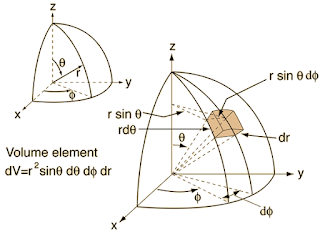
\includegraphics[scale=0.7,angle=0]{sphcoordel.png}
\caption{Spherical Volume Element}
\label{sphvol}
\end{center}
\end{figure}
This volume element is a type of box, so we need to find the dimensions of the box to find the element. The figure says $r$ but in our case assume $r$ in the figure is $\rho$. It also switches our $\phi$ and $\theta$. So if we take $\rho \sin(\phi)$ that gives us the projection of the radius onto the $xy$-plane. Then by rotating that through an angle $d\theta$ on the plane that gives us our first dimension, the side of the box that turns in the $\theta$ direction. Then we can find the $\phi$ dimension by rotating $\rho$ through $d\phi$, which gives $\rho \, d\phi$. Finally the outward direction is just $d\phi$. To find the volume we multiply everything and that gives:
\begin{gather*}
    dV = (\rho \sin(\phi) \,d \theta)(\rho \,d\phi)(d\rho) = \rho^2 \sin(\phi) \,d\theta \, d\phi\, d\rho
\end{gather*}
Now we can easily figure out the triple integral using $\rho \in [a,b]$, $\theta \in [\alpha, \beta]$ and $\phi \in [c,d]$:
\begin{gather*}
    \iiint_E f(x,y,z)\, dV = \int_c^d \int_\alpha^\beta \int_a^b f(\rho\sin(\phi)\cos(\theta), \rho\sin(\phi)\cos(\theta), \rho\cos(\phi)) \, \rho^2 \sin(\phi) \,d\rho\, d\theta\,d\phi
\end{gather*}
Normally spherical coordinates are used when the solid regions or surfaces of integration are spheres or cones(since those would work with $\rho$ or $\phi$).

\textbf{Important: }Make sure that you don't forget the $\rho^2 \sin(\phi)$ factor in the integral. This is just like the extra $r$ in polar or cylindrical integration, except a little more complicated.
\subsection{Change of Variables in Multiple Integrals}
\subsubsection{Double Integrals}
With single integrals we simplified them by making a \textbf{u-substitution}. We can do something similar for double integrals by making a \textbf{change of variables}. We've already seen this in action when converting to polar coordinates. We use:
\begin{gather*}
    x = r \cos(\theta)\hspace{20pt}y = r\sin(\theta)
\end{gather*}
We convert from the integration region in the $xy$ plane to a new region in the $r\theta$ plane, and this is called a \textbf{transformation}. A transformation is just a function who's domain and range are a plane. If no two input points have the same output, then it is \textbf{one-to-one}. If this is the case, then a transformation $T$ has an \textbf{inverse transformation} $T^{-1}$ to go backwards.

Imagine a transformation from $(u,v) \to (x,y)$ with two functions, $x = g(u,v)$ and $y = h(u,v)$. We could define a vector which defines the new region:
\begin{gather*}
    \vv{r} = g(u,v)\hat{i} + h(u,v)\hat{j}
\end{gather*}
To find the tangent parallelogram to the new region(it's not a plane because the region is confined), we need to pretend it is a tangent plane and write out two vectors like so:
\begin{gather*}
    \vv{r_u} = g_u\hat{i} + h_u\hat{j}\\
    \vv{r_v} = g_v\hat{i} + h_v\hat{j}
\end{gather*}
Now if you want to compute the change in the plane, the new tangent parallelogram is formed by:
\begin{gather*}
    \Delta u \,\vv{r_u}\\
    \Delta v \,\vv{r_v}
\end{gather*}
To find the area of the parallelogram you just take the cross product:
\begin{gather*}
    |(\Delta u \,\vv{r_u}) \times (\Delta v \,\vv{r_v})| \implies |\vv{r_u} \times \vv{r_v}| = \begin{vmatrix}
        \dfrac{\p x}{\p u} && \dfrac{\p x}{\p v}\\\\
        \dfrac{\p y}{\p u} && \dfrac{\p y}{\p v}
    \end{vmatrix}\hat{k}
\end{gather*}
This special determinant is called the \textbf{Jacobian} of the transformation and has some special notation:
\begin{gather*}
    \frac{\p (x,y)}{\p (u,v)}
\end{gather*}
Finally we can tie it all together to find the area element:
\begin{gather*}
    \Delta A = \bigg|\frac{\p (x,y)}{\p (u,v)}\bigg| \Delta u \Delta v \implies dA = \bigg|\frac{\p (x,y)}{\p (u,v)}\bigg| \,du\, dv
\end{gather*}
So the change of variables(or u,v substitution) for a double integral is:
\begin{gather*}
    \iint_R f(x,y) \, dA = \iint_S f(x(u,v),y(u,v)) \,\bigg|\frac{\p (x,y)}{\p (u,v)}\bigg| \, du \, dv
\end{gather*}
In fact, if you use this with $x = r\cos(\theta)$ and $y = r\sin(\theta)$ you will get the formula for polar coordinate double integration. The normal rectangle region will get transformed into the polar rectangle.
\subsubsection{Triple Integrals}
The process for triple integrals is similar, except now you have a transformation carried out by three functions of three variables, with one new function $z(x,y,w)$. The Jacobian is the same except for a new row for $z$ and a new column for the new variable $w$. So you can quite easily see:
\begin{gather*}
    \iiint_R f(x,y,z) \, dV = \iiint_S f(x(u,v,w), y(u,v,w), z(u,v,w)) \,\bigg|\frac{\p (x,y,z)}{\p (u,v,w)} \bigg| \,du\,dv\,dw
\end{gather*}
\newpage
\section{Vector Calculus}
\subsection{Vector Fields}
A \textbf{vector field} is a field which associates every point in space with a vector that has magnitude and direction. One type of vector field is a \textit{force field} where the vector being used is a force vector.

We can define a vector field to be a function which assigns each point in its domain $D$ to a vector $\vv{F}$. We can visualize a vector field by drawing the vector at representative points to get general idea of how it looks.

We can define the vector function $\vv{F}(x,y)$ for 2D in terms of two scalar(normal) functions $P$ and $Q$, where:
\begin{gather*}
    \vv{F} = P\,\hat{i} = Q\,\hat{j}
\end{gather*}
A vector function is continuous if it's component functions are continuous. In general, you can assign each point its position vector $\vv{x} = \vl x,y,z \vr$ and then write $\vv{F}(\vv{x})$.
\subsubsection{Gradient Fields}
Remember the gradient function from Chapter 15, where the gradient is a vector. Effectively since the gradient is a vector that depends on the point, we can use the gradient as a vector field which is called the \textbf{gradient field}.
\begin{gather*}
    \vv{F}(\vv{x}) = \n f(x,y,z) = f_x \, \hat{i} + f_y \, \hat{j} + f_z \, \hat{k}
\end{gather*}
A vector field is called a \textbf{conservative field} if it can be written as the gradient of some scalar function, where $\vv{F} = \n f$. Here $f$ is called the \textbf{potential function}(see the relationship here between force and potential). For example, the gravitational force can be written as the gradient of a potential function. Remember the formula for gravitational potential energy:
\begin{gather*}
    U_g = \frac{GMm}{r} = \frac{GMm}{\sqrt{x^2 + y^2 + z^2}}\\
    \n U_g = \frac{-GMmx}{(x^2 + y^2 + z^2)^{3/2}}\,\hat{i}+\textrm{y and z components}= \vv{F_g}
\end{gather*}
\subsection{Line Integrals}
You can think about a single integral as integrating where the 'region' is just a line. But what if the line is just a general case? What if you want to integrate values of a function over a curve? This could be useful when you're working with wires and magnetism. Using a curve $C$ which is given in 2D by:
\begin{gather*}
    x=x(t)\hspace{40pt}y=y(t)\hspace{40pt}a \leqslant t \leqslant b\\
    \vv{r}(t) = x(t)\,\hat{i} + y(t)\,\hat{j}
\end{gather*}
Assuming that this is a smooth curve, we can divide the curve into smaller and smaller elements $\Delta s$ and eventually we get the \textbf{line integral}:
\begin{gather*}
    \int_C f(x,y) \,ds = \lim_{n \to \infty}\sum_{i=1}^n f(x_i,y_i) \, \Delta s
\end{gather*}
Remember that:
\begin{gather*}
    L = \int_C ds = \int_a^b \sqrt{\bigg(\frac{dx}{dt}\bigg)^2 + \bigg(\frac{dy}{dt}\bigg)^2} \,dt
\end{gather*}
Finally, to parametrize a curve we can find the final form of the \textbf{line integral with respect to arc length}:
\begin{gather*}
    \int_C f(x,y)\,ds = \int_a^b f(x(t),y(t))\,\sqrt{\bigg(\frac{dx}{dt}\bigg)^2 + \bigg(\frac{dy}{dt}\bigg)^2} \,dt
\end{gather*}
To check that this works, we can parametrize with $t = x$ and see if we get the normal single integral:
\begin{gather*}
    \int_C f(x,y)\,ds \implies \int_a^b f(x) \,dx
\end{gather*}
\begin{figure}[H]
\begin{center}
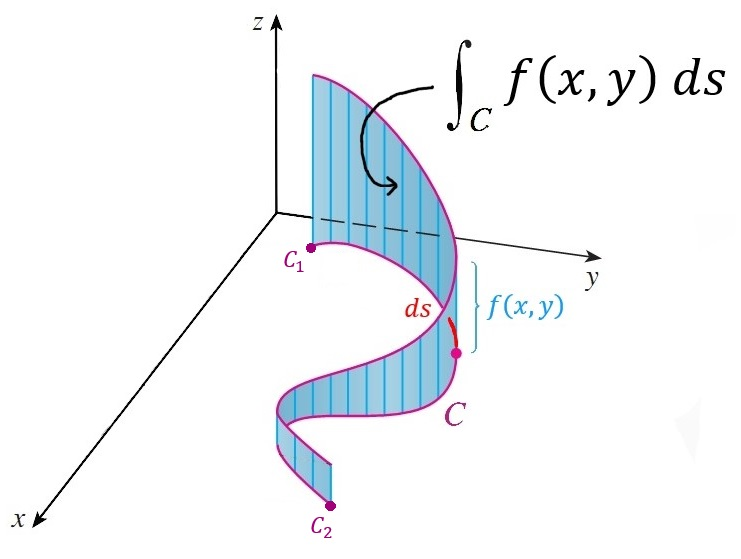
\includegraphics[scale=0.3]{LineInt.jpg}
\caption{Line Integrals Geometrically}
\label{lineint}
\end{center}
\end{figure}
If $C$ is a \textbf{piecewise-smooth curve}(which means it's made up of many smooth curves connected) then the following should be obvious:
\begin{gather*}
    \int_C f(x,y)\,ds = \int_{C_1} f\,ds + \int_{C_2} f\,ds + \int_{C_3} f\,ds...
\end{gather*}
Physical interpretations of the line integral depend on the function being integrated. For example, Integrating density gives you mass and center of mass.

Sometimes you will need to calculate line integrals \textbf{with respect to x or y}. Think about what this means, you are only counting the changes in the $x$-direction but not the $y-direction$. So if the normal line integral is the area of the 'curtain' then:
\begin{figure}[H]
\begin{center}
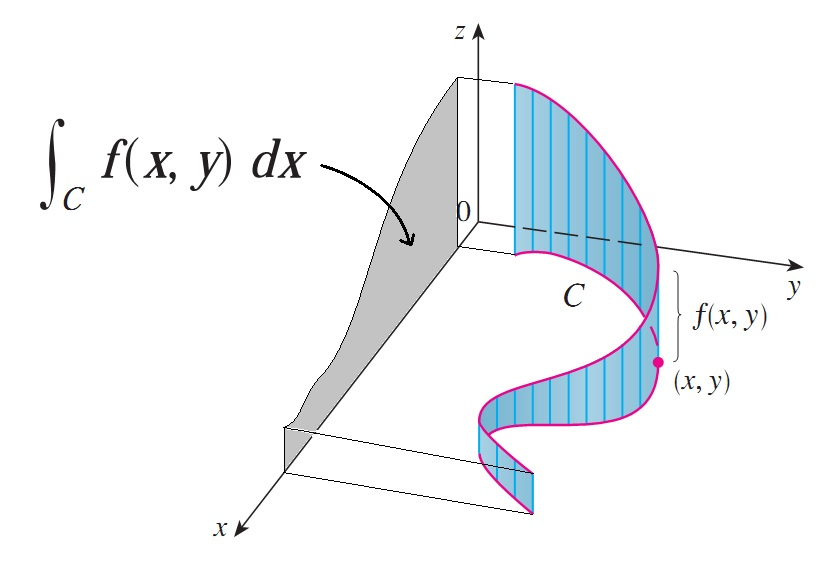
\includegraphics[scale=0.3]{Linedx.jpg}
\caption{Line Integral With Respect To $x$}
\label{linedx}
\end{center}
\end{figure}
By using the fact that $dx = \frac{dx}{dt}\,dt$:
\begin{gather*}
    \int_C f(x)\,dx = \int_C f(x(t))\,x'(t)\,dt
\end{gather*}
Sometimes when you have integrals with respect to $x$ and $y$ they can be written together:
\begin{gather*}
    \int_C\,f\,dx + \int_C\,g\,dy = \int_C f\,dx + g\,dy
\end{gather*}
Remember this is \textit{just} a shorthand.

When setting up line integrals, parametrizing curves is an important skill, one frequent parametrization is over a line. Given two points, the vector representation:
\begin{gather*}
    \vv{r}(t) = (1-t)\vv{r_0} + \vv{r_1}t\hspace{20pt}t \in [0,1]
\end{gather*}
When integrating with respect to a variable, you can get different answers based on the direction you're going in, or the curve's \textbf{orientation}.
\begin{gather*}
    \int_{-C}\,f\,dx = -\int_C\,f\,dx
\end{gather*}
However, this does not apply when integrating over arc length because $ds$ is always positive, while $dx$ can go in any direction.
\subsubsection{Line Integrals in Space}
For a curve given by $\vv{r}(t) = \vl x(t),y(t),z(t) \vr$ then in 3D we can say:
\begin{gather*}
    \int_C f\,ds = \int_a^b\,f(x(t),y(t),z(t))\,\sqrt{\bigg(\frac{dx}{dt}\bigg)^2 + \bigg(\frac{dy}{dt}\bigg)^2 + \bigg(\frac{dz}{dt}\bigg)^2}\,dt
\end{gather*}
Or more generally you can write:
\begin{gather*}
    \int_a^b f(\vv{r}(t))\,|\vv{r}'(t)| \,dt
\end{gather*}
\subsubsection{Line Integrals in Vector Fields}
To calculate the work done by a force $\vv{F}$ we can find work as $W = \vv{F} \vdot \vv{D}$. The force vector is obvious, but the displacement vector you need to approximate when $ds$ is small, which would be the \textbf{unit tangent vector} $\vv{T}$. It's a unit vector because you don't want to weight different parts of the curve more or less. So:
\begin{gather*}
    W = \int_C \vv{F} \vdot \vv{T}\,ds
\end{gather*}
More generally for any continuous vector field:
\begin{gather*}
    W = \int_C \vv{F} \vdot \vv{T}\,ds = \int_a^b \vv{F}(\vv{r}(t)) \,\frac{\vv{r}'(t)}{|\vv{r}'(t)|}\,dt = \int_a^b \vv{F}\,(\vv{r}(t)) \vv{r}'(t) \,dt = \int_C \vv{F}\,d\vv{r}
\end{gather*}
Remember that when using the $d\vv{r}$ form the integral needs the negative sign because $\vv{T}$ becomes negative when $C$ does.
\subsection{The Fundamental Theorem For Line Integrals}
From single-variable calculus,
\begin{gather*}
    \int_a^b f'(x)\,dx = f(b)-f(a)
\end{gather*}
This should make sense because adding up the individual rates of change is going to give you the total net change.

Similarly, if $C$ is a smooth curve defined by $\vv{r}(t)$ and $f$ is a differentiable function, whose gradient vector is continuous on $C$:
\begin{gather*}
    \int_C\n f\,d\vv{r} = f(\vv{r}(b)) - f(\vv{r}(a))
\end{gather*}
This means that you can evaluate the line integral over a conservative vector field just by knowing the endpoint values. We can prove this by using the chain rule and the original FTC:
\begin{gather*}
    \int_C \n f\,d\vv{r} = \int_a^b \n f(\vv{r}(t)) \,\vv{r}'(t)\,dt\\
    = \int_a^b \bigg(\frac{\p f}{\p x}\frac{dx}{dt} + \frac{\p f}{\p y}\frac{dy}{dt} + \frac{\p f}{\p z}\frac{dz}{dt}\bigg)\,dt\\
    = \int_a^b \frac{d}{dt} f(\vv{r}(t))\,dt\\
    = f(\vv{r}(b)) - f(\vv{r}(a))
\end{gather*}
Step 3 here is because of the chain rule in reverse and the final step is just the normal FTC.
\subsubsection{Path Independence}
An obvious consequence of this FTC is that for conservative vector fields, the path taken does not matter as long as you have the same initial and final points. A vector function $\vv{F}$ is called path independent if $\int_C \vv{F}\,d\vv{r}$ is the same for any path with the same endpoints.

Now if we imagine a \textbf{closed curve}, which is a curve that connects to itself(which means it technically does not have endpoints). However, if we split the curve into 2 curves using two endpoints(so one curve goes $A\rightarrow B$ and the other $B \rightarrow A$). Then adding those line integrals should give zero because their endpoints are switched. So,

$\int_C \vv{F}\,d\vv{r}$ is \textbf{path independent} if and only if $\int_D \vv{F}\,d\vv{r} = 0$ for any closed path $D$ in the domain.

An \textbf{open region} is a region where every point inside it is contained in a disk that is contained within the region. This means that any boundary points cannot be included(because then you can't have a disk). If you have a path independent vector field on that open region that is continuous, then you can say that the vector field is conservative on that region.
\begin{proof}
If we choose an open region $D$, then there must be a disk around any point $(x,y)$ in $D$. If you choose another point to the left of the point $(x_1,y)$ where $x_1 < x$. Then choose any other path $C_2$ from the initial point $(a,b)$ since the function is path independent it shouldn't matter. Then let $f$:
\begin{gather*}
    f(x,y) = \int_{C_1} \vv{F}\,d\vv{r} + \int_{C_2}\vv{F}\,d\vv{r} = \int_{(a,b)}^{(x_1,y)}\vv{F}\,d\vv{r} + \int_{C_2}\vv{F}\,d\vv{r}
\end{gather*}
Since the first integral doesn't depend on $x$, we can take the partial derivative of $f$ on both sides and that first integral will zero out.
\begin{gather*}
    \frac{\p}{\p x}f(x,y) = 0 + \frac{\p}{\p x}\int_{C_2}\vv{F}\,d\vv{r}
\end{gather*}
Because $C_2$ is horizontal, $dy = 0$ and so there is no relevant $y$-component to $\vv{F}$. This means that we can rewrite $\vv{F}\,d\vv{r}$ as just the scalar function $P\,dx$. Using a parameter $t$ so we can use FTC:
\begin{gather*}
    \frac{\p}{\p x}f(x,y) = \frac{\p}{\p x}\int_{C_2}P\,dx = \frac{\p}{\p x}\int_{x_1}^x P(t,y)\,dt = P(x,y)
\end{gather*}
The last step is because of the original FTC. Similarly we can show using a vertical line as $C_2$ that:
\begin{gather*}
    \frac{\p}{\p y}f(x,y) = Q(x,y)
\end{gather*}
Now since $\vv{F} = \vl P,Q \vr = \vl f_x, f_y \vr$, $\n f = F$ and so $\vv{F}$ is conservative.
\end{proof}
If $\vv{F} = \vl P, Q \vr$ is conservative, then we can write for $\vv{F} = \n f$:
\begin{gather*}
    P = \frac{\p f}{\p x}\hspace{40pt}Q = \frac{\p f}{\p y}
\end{gather*}
So by taking the other variable's derivative on both equations, and using the fact that the order of the derivatives doesn't matter:
\begin{gather*}
    \frac{\p P}{\p y} = \frac{\p^2 f}{\p y \p x} = \frac{\p Q}{\p x}
\end{gather*}
If the converse of this is true, then we can use this to find if a vector field is conservative. However, in order to make this work we need stricter conditions, so we define a \textbf{simple curve} to be one that doesn't intersect itself(like an infinity sign would not be simple). We can also define a \textbf{simply-connected region}(for use in 3D stuff) to be such that any simple closed curve in the region that you can draw between two points never leaves the region. This means no holes, gaps, or divisions.

So if the vector field satisfies the partial derivative condition and it is present on the open simply-connected region then we can say it is conservative. The reason for this is discussed in 17.4.

Now to actually find the potential function $f$(where $\vv{F} = \n f$, we can use \textbf{partial integration}(which is really just normal single integration)) to get one variable but you will need to deal with the '+C' issues because a constant with respect to one variable can still be a function of the other two.
\subsubsection{Conservation of Energy}
We can use the ideas of this section to show how energy is conserved in a conservative field. Using Newton's Second Law:
\begin{gather*}
    \vv{F} = m\vv{a} = m\vv{r}''(t)\\
    W_k = \int_C \vv{F}\,d\vv{r} = \int_a^b \vv{F}(\vv{r}(t)) \vv{r}'(t)\,dt = \int_a^b m\vv{r}''(t)\vdot \vv{r}'(t)\,dt
\end{gather*}
Now using the identity $\vv{r}'(t) \vdot \vv{r}''(t) + \vv{r}''(t)\vdot \vv{r}'(t) = 2\vv{r}'(t)\vdot\vv{r}''(t) = \dfrac{d}{dt} \bigg[\vv{r}'(t) \vdot \vv{r}'(t)\bigg] = \dfrac{d}{dt}\bigg|\vv{r}'(t)\bigg|^2$
\begin{gather*}
    = \frac{1}{2}m\int_a^b\dfrac{d}{dt}\bigg|\vv{r}'(t)\bigg|^2\,dt = \frac{1}{2}m\bigg[|\vv{r}'(b)|^2 - |\vv{r}'(a)|^2\bigg]
\end{gather*}
Since $\vv{r}'(t)$ is just velocity, this shows how $W = \Delta \frac{1}{2}mv^2 = \Delta KE$. Now we can define potential energy as the potential function where $\vv{F} = -\n P$, which makes sense because work is the negative of the change in PE.
\begin{gather*}
    W_p = \int_C \vv{F}\,d\vv{r} = -\int_C \n P\,d\vv{r} = P(a)-P(b)
\end{gather*}
Adding these two equations proves the \textbf{conservation of energy}:
\begin{gather*}
    P(a) + K(a) = P(b) + K(b)
\end{gather*}
\subsection{Green's Theorem}
\textbf{Green's Theorem} is useful because it provides a connection between the line integral of the border of a region and the double integral over that region. To use this we need to have \textbf{positive orientation}, which simply means always going counterclockwise so the region is always on the left.

If $C$ is a positively oriented, piecewise-smooth, simple closed curve in a plane and $D$ is a region bounded by $C$. If $P$ and $Q$ have continuous partial derivatives on the open region that contains $D$, then:
\begin{gather*}
    \oint_C P\,dx + Q\,dy = \iint_D \bigg(\frac{\p Q}{\p x} - \frac{\p P}{\p y}\bigg)\,dA
\end{gather*}
The new integral notation simply signifies a line integral in the positively oriented direction. Also the notation $\p D$ is used to signfiy the border of $D$. To prove this, let's define a region that can be expressed as a combination of type I and type II, called a \textbf{simple region}.
\begin{proof}
To prove Green's Theorem, we will need to split up the integral and prove that:
\begin{gather*}
    \oint_C P\,dx = -\iint_D \frac{\p P}{\p y}\,dA\\
    \oint_C Q\,dy = \iint_D \frac{\p Q}{\p x}\,dA
\end{gather*}
So to prove the first one we can express $D$ as a type I region(bounded by two functions of $y$). So using the partial FTC:
\begin{gather*}
    \iint_D \frac{\p P}{\p y}\,dA = \int_a^b\int_{g_1(y}^{g_2(y)}\frac{\p P}{\p y}\,dy\,dx = \int_a^b P(x,g_2(x)) - P(x,g_1(x))\,dx
\end{gather*}
So now to get the line integral, we can split the region into 4 curves, two that go up and down, and 2 that are defined by $g_1(y)$ and $g_2(y)$. Since we're going counterclockwise, one of the $g$-functions will be going the right way and one the wrong way. So we add the negative sign to it to work.
\begin{gather*}
    \oint_{C_1}P(x,y)\,dx = -\int_a^b P(x,g_2(x))\,dx\\
    \oint_{C_3}P(x,y)\,dx = \int_a^b P(x,g_1(x))\,dx
\end{gather*}
Now because the other 2 curves are vertical, they won't have any $dx$ so they don't contribute to the integral in the $x$-direction. So we can write:
\begin{gather*}
    \oint_C P(x,y)\,dx = \int_a^b P(x,g_1(x))\,dx - \int_a^b P(x,g_2(x))\,dx
\end{gather*}
Comparing the two equations we got, we can see how:
\begin{gather*}
    \oint_C P(x,y)\,dx = -\iint_D \frac{\p P}{\p y}\,dA
\end{gather*}
\end{proof}
When using this theorem, sometimes the line integral or the double integral might be easier to evaluate. For example, if both $P$ and $Q$ are zero on the \textbf{boundary}, then the line integral and the double integral will always be zero.

You can use it to find areas if you can find $P$ and $Q$ which make the integrand $1$. When you apply some possibilities:
\begin{gather*}
    \iint_D \,dA = A = \oint_C x\,dy = -\oint_C y\,dx = \frac{1}{2}\oint_C x\,dy - y\,dx
\end{gather*}
If you want to use Green's Theorem on a region with holes you can do that by adding up smaller regions that work with the theorem. The theorem can be extended to show that this works.
\subsubsection{Consequences of Green's Theorem}
Last section, we needed to prove that if $\vv{F} = \vl P,Q \vr$ is on an open simply connected region, and both scalar functions have continuous partial derivatives(1st order) and that:
\begin{gather*}
    \frac{\p P}{\p y} = \frac{\p Q}{\p x}
\end{gather*}
Then we can see how:
\begin{gather*}
    \oint_C \vv{F}\,d\vv{r} = \oint_C P\,dx + Q\,dy = \iint_R \bigg(\frac{\p Q}{\p x} - \frac{\p P}{\p y}\bigg)\,dA = \iint_R 0\,dA = 0
\end{gather*}
So if the field does no work while going around the curve, then $\vv{F}$ is conservative.
\subsection{Curl and Divergence}
Now we can define operations that can be performed \textit{on} vector fields.
\subsubsection{Curl}
If $\vv{F} = P\,\hat{i} + Q\,\hat{j} + R\,\hat{k}$ is a 3D vector field, with continuous first partial derivatives, then the \textbf{curl} $\curl{\vv{F}}$ is:
\begin{gather*}
    \curl \vv{F} = \bigg(\frac{\p R}{\p y} - \frac{\p Q}{\p z}\bigg)\,\hat{i} + \bigg(\frac{\p P}{\p z} - \frac{\p R}{\p x}\bigg)\,\hat{j} + \bigg(\frac{\p Q}{\p x} - \frac{\p P}{\p y}\bigg)\,\hat{k}
\end{gather*}
You can think of the $\n$ operator as acting as the partial operator for each unit vector in each direction.
So the notation for the \textbf{curl} should make sense because it is basically a determinant:
\begin{gather*}
    \curl \vv{F} = \begin{bmatrix}
    \hat{i} & \hat{j} & \hat{k}\\
    \vspace{2pt}
    \dfrac{\p}{\p x} & \dfrac{\p}{\p y} & \dfrac{\p }{\p z}\\
    \vspace{5pt}
    P & Q & R\\
    \end{bmatrix}
\end{gather*}
Now using curl, we can say that if $f$ is a 3D with continuous second partial derivatives:
\begin{gather*}
    \curl (\n f) = 0
\end{gather*}
\begin{proof}
    $\curl (\n f) = \begin{bmatrix}
    \hat{i} & \hat{j} & \hat{k}\\
    \vspace{2pt}
    \dfrac{\p}{\p x} & \dfrac{\p}{\p y} & \dfrac{\p }{\p z}\\
    \vspace{5pt}
    \dfrac{\p f}{\p x} & \dfrac{\p f}{\p y} & \dfrac{\p f}{\p z}\\
    \end{bmatrix}
    = \bigg(\dfrac{\p^2 f}{\p y\p z} - \dfrac{\p^2 f}{\p z\p y}\bigg)... = 0$
\end{proof}
Because any conservative field would have $\n f$, we can say that if $\vv{F}$ is conservative, then $\curl \vv{F} = 0$.

The converse of this is only true if $\vv{F}$ is defined everywhere, or if the domain is simply connected(no gaps), so if this is true and all $P,Q,R$ have continuous partial derivatives, if $\curl \vv{F} = 0$, then $\vv{F}$ is conservative.

\begin{figure}[H]
\begin{center}
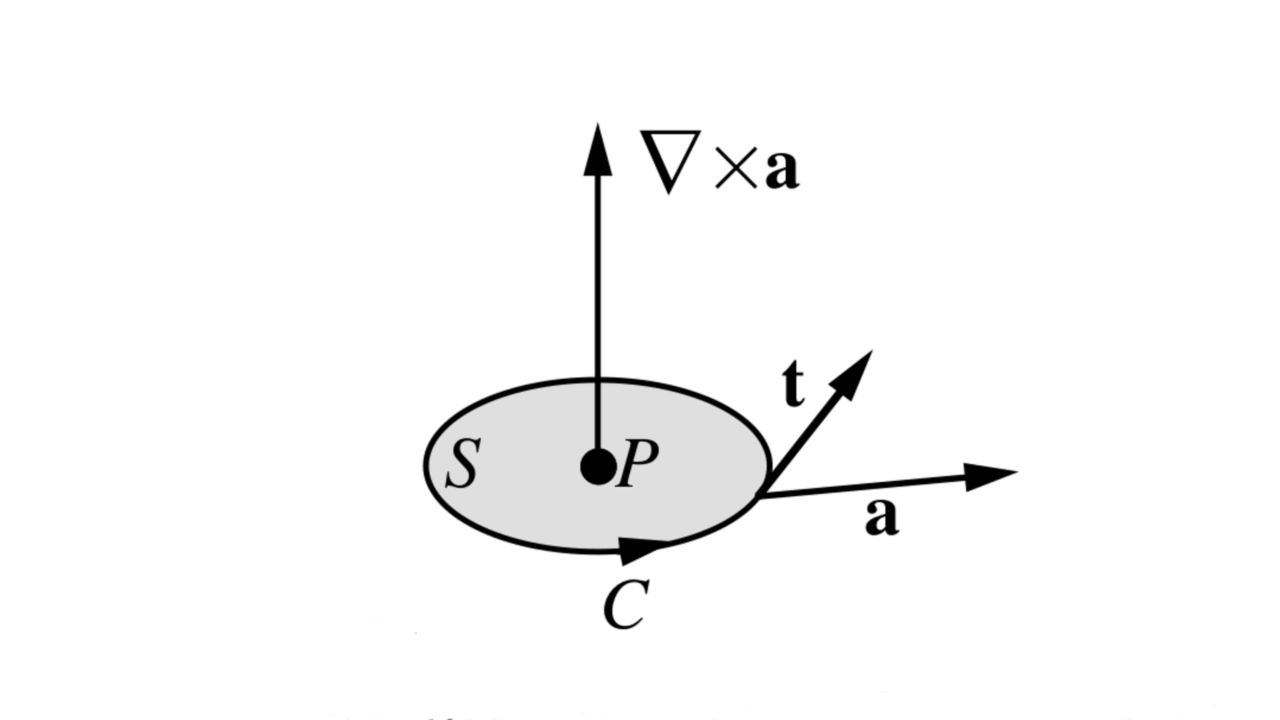
\includegraphics[scale=0.15]{curl.png}
\caption{Curl Geometrically}
\label{curl}
\end{center}
\end{figure}
The curl vector is named so because it has significance with rotations. Think of a fluid that flows in the direction out of the circle(think of that as a cross section of a pipe). If $\curl \vv{F} = 0$, then at that point the fluid is only moving straight, not rotating at all. If it does not, then the fluid particles rotate as well, the direction of the curl vector specifies the direction of rotation(right hand rule).
\subsubsection{Divergence}
Given $\vv{F} = \vl P,Q,R \vr$, and the first partial derivatives exist, then the \textbf{divergence of} $\vv{F}$ is:
\begin{gather*}
    \diver \vv{F} = \frac{\p P}{\p x} + \frac{\p Q}{\p y} + \frac{\p R}{\p z}
\end{gather*}
This notation should make sense since it's just a dot product of the operator $\n$ and the vector field, which produces a \textit{scalar field}.

If the second order partial derivatives are continuous, then we can say that:
\begin{gather*}
    \diver(\curl \vv{F}) = 0
\end{gather*}
This can easily be proved by applying the definitions of the two operations and the terms will cancel out because of Clairaut's Theorem.

The physical interpretation of this would be the change in the mass of a fluid per unit volume at a point. In other words, it measures the \textbf{compressibility}, or the tendency of the fluid to diverge from the point. So if $\diver \vv{F} = 0$, then we can say that the fluid is \textbf{incompressible}.

If you try to take the divergence of a graident you get:
\begin{gather*}
    \diver \n f = \frac{\p^2 f}{\p x^2} + \frac{\p^2 f}{\p y^2} + \frac{\p^2 f}{\p z^2}
\end{gather*}
We have seen this before, in the \textbf{Laplacian} operator, which works with the notation, since $\n^2 f = \n \vdot \n$.
\subsubsection{Vector Forms of Green's Theorem}
These two new operators allow us to rewrite Green's Theorem in a way that is more useful for vector calculus. So starting with the integral:
\begin{gather*}
    \oint_C \vv{F}\,d\vv{r} = \oint_C P\,dx + Q\,dy
\end{gather*}
The curl would be:
\begin{gather*}
    \curl \vv{F} = \begin{bmatrix}
    \hat{i} & \hat{j} & \hat{k}\\
    \vspace{2pt}
    \dfrac{\p}{\p x} & \dfrac{\p}{\p y} & \dfrac{\p }{\p z}\\
    \vspace{5pt}
    P & Q & 0\\
    \end{bmatrix}
    = \bigg(\frac{\p Q}{\p x} - \frac{\p P}{\p y}\bigg)\,\hat{k}\\
    (\curl \vv{F})\vdot \hat{k} = \bigg(\frac{\p Q}{\p x} - \frac{\p P}{\p y}\bigg)\,\hat{k} \vdot \hat{k} = \bigg(\frac{\p Q}{\p x} - \frac{\p P}{\p y}\bigg)
\end{gather*}
Therefore, we can use this in the right side of Green's Theorem:
\begin{gather*}
    \oint_C \vv{F}\,d\vv{r} = \iint_D (\curl \vv{F})\vdot \hat{k}\,dA
\end{gather*}
The above equation uses $d\vv{r}$, the \textbf{tangential} component of $\vv{F}$ along $C$, now we can get a second formula that uses the \textbf{normal} component to $C$:
\begin{gather*}
    C: \vv{r}(t) = x(t)\,\hat{i} + y(t)\,\hat{j}\\
    \vv{T}(t) = \frac{x'(t)}{|\vv{r}'(t)|}\,\hat{i} + \frac{y'(t)}{|\vv{r}'(t)|}\,\hat{j}
\end{gather*}
So it can be shown that the unit normal vector $\vv{n} = \frac{\vv{T}'(t)}{|\vv{T}'(t)|}$:
\begin{gather*}
    \vv{n} = \frac{y'(t)}{|\vv{r}'(t)|}\,\hat{i} + \frac{x'(t)}{|\vv{r}'(t)|}\,\hat{j}
\end{gather*}
So using $\frac{ds}{dt} = |\vv{r}'(t)|$:
\begin{gather*}
    \oint_C (\vv{F}\vdot \vv{n})\,ds = \int_a^b (\vv{F}\vdot\vv{n})\,|\vv{r}'(t)|\,dt = \int_a^b P(x(t),y(t))\,y'(t) - Q(x(t),y(t))\,x'(t)\,dt \\= \oint_C P\,dx - Q\,dx = \iint_D\bigg(\frac{\p P}{\p x} + \frac{\p Q}{\p y}\bigg)\,dA
\end{gather*}
So this means:
\begin{gather*}
    \oint_C \vv{F}\vdot\vv{n}\,ds = \iint_D \diver \vv{F}(x,y)\,dA
\end{gather*}
This version means that the line integral of the \textbf{normal} component of $\vv{F}$ along $C$ is equal to the double integral of the divergence of $\vv{F}$ over $D$.
\subsection{Parametric Surfaces and Their Areas}
\subsubsection{Parametric Surfaces}
To describe more general surfaces, we can use parametric equations in which case they are called \textbf{parametric surfaces}, which we can use two parameters $u$ and $v$.
\begin{gather*}
    \vv{r}(u,v) = x(u,v)\,\hat{i} + y(u,v)\,\hat{j} + z(u,v)\,\hat{k}
\end{gather*}
As $u$ and $v$ vary, each point will give a point on $S$, which is traced out by $\vv{r}$.
\begin{figure}[H]
\begin{center}
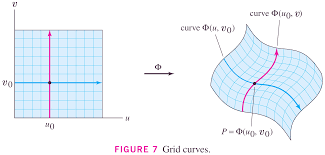
\includegraphics[scale=0.9]{gridcurves.png}
\caption{Grid Curves}
\label{gridcurves}
\end{center}
\end{figure}
There are two useful groups of curves, called \textbf{grid curves} that use constant values of one parameter, say if we make $u = u_0$ and let $v$ vary. This creates a curve given by $\vv{r}(u_0,v)$($\Phi$ in the figure). Parametric equations are useful in order to solve the problem of how to express a surface in terms of equations. Just a note, to express $z = f(x,y)$ in parametric equations, we can just use:
\begin{gather*}
    x = x\hspace{20pt}y=y\hspace{20pt}z= f(x,y)
\end{gather*}
\subsubsection{Surfaces of Revolution}
Let's consider a simple case of rotating the curve $y = f(x)$ around the $x-axis$, where $f(x) \geqslant 0$ for now. Let $\theta$ be the angle of rotation. If $(x,y,z)$ is an arbitrary point,
\begin{gather*}
    x = x\hspace{20pt}y = f(x)\,\cos(\theta)\hspace{20pt}z = f(x)\,\sin(\theta)
\end{gather*}
(because $z$ is the height, etc.)
\subsubsection{Tangent Planes}
Remember the general parametric surface:
\begin{gather*}
    \vv{r}(u,v) = x(u,v)\,\hat{i} + y(u,v)\,\hat{j} + z(u,v)\,\hat{k}
\end{gather*}
At the point ($u_0,v_0$), we can find the tangent vector:
\begin{gather*}
    \vv{r_v} = \frac{\p x}{\p v}\,\hat{i} + \frac{\p y}{\p v}\,\hat{j} + \frac{\p z}{\p v}\,\hat{k}\\
    \vv{r_u} = \frac{\p x}{\p u}\,\hat{i} + \frac{\p y}{\p u}\,\hat{j} + \frac{\p z}{\p u}\,\hat{k}\\
\end{gather*}
If $\vv{r_u} \times \vv{r_v} \neq 0$, then the surface is a \textbf{smooth surface}, and the plane's normal vector is given by that cross product.
\subsubsection{Surface Area}
We can approximate the surface's infinitesimal element as a parallelogram, so the surface area element would be:
\begin{gather*}
    |\vv{r_u} \times \vv{r_v}|\,du\,dv
\end{gather*}
So we can write the surface area of a general parametric surface as:
\begin{gather*}
    A(S) = \iint_D |\vv{r_u} \times \vv{r_v}|\,du\,dv
\end{gather*}
\subsubsection{Infinitestimal Surface Area}
Using this surface area formula, we can express $dA$ as a general expression:
\begin{gather*}
    d\vv{A} = (\vv{r_u} \times \vv{r_v})\,du\,dv
\end{gather*}
This gives us a way to find $d\vv{A}$ in any coordinate system with parameters such as these. In fact, this is an idea that connects to the Jacobian. For example, in cartesian we know that $\vv{r_x} = \hat{i}$ and $\vv{r_y} = \hat{j}$. So the cross product $\hat{i} \times \hat{j} = \hat{k}$. So $d\vv{A}$ in cartesian:
\begin{gather*}
    d\vv{A} = dx\,dy\,\hat{k}
\end{gather*}
We can apply this to any of the other coordinate systems as well. For 3+ parameter systems, we can use the Jacobian to convert.
\subsubsection{Surface Area of the Graph of a Function}
For the special case of $z = f(x,y)$, we can use the parametric equations described previously and solve:
\begin{gather*}
    A(S) = \iint_D \sqrt{1 + \bigg(\frac{\p z}{\p x}\bigg)^2 + \bigg(\frac{\p z}{\p y}\bigg)^2}\,dA
\end{gather*}
To check if this agrees with the single-variable formula for surfaces of revolution, use:
\begin{gather*}
    x=x\hspace{20pt}y = f(x)\,\cos(\theta)\hspace{20pt}z=f(x)\,\sin(\theta)
\end{gather*}
After you perform the cross product and solve, you get:
\begin{gather*}
    A = 2\pi \int_a^b f(x)\,\sqrt{1 + (f'(x))^2}\,dx
\end{gather*}
This is the exact formula used in single-variable calculus, so this does agree.
\subsection{Surface Integrals}
The connection between surface integrals and surface area is similar to line integrals and arc length. The integral is just integrating \textit{something} over the whole space. So the form for the surface integral would be:
\begin{gather*}
    \iint_S f(x,y,z)\,dS = \lim_{m,n \to \infty} \sum_{i = 1}^m \sum_{j = 1}^n f(P_{ij})\,\Delta S
\end{gather*}
\subsubsection{Graphs}
If the surface is a graph with $z = g(x,y)$, you can account for the curvature of that surface by approximating as before. Using the cross product with the parallelogram gets you:
\begin{gather*}
    \iint_S f(x,y,z)\,dS = \iint_D f(x,y,g(x,y)) \sqrt{(g_x)^2 + (g_y)^2 + 1}\,dA
\end{gather*}
Notice how that functions as a correction factor(think like the Jacobian transformation style). You can do this with the $yz$ projection as well by changing the correction factor to have the partials of the variables not used.

The applications of these are similar, for example if I have a thin sheet(thickness is negligible), I can find the total mass of it:
\begin{gather*}
    m = \iint_S \rho(x,y,z)]\,dS
\end{gather*}
This sheet will have \textbf{center of mass}, for example $\bar{x} = \dfrac{1}{m}\iint_S x\rho(x,y,z)\,dS$
\subsubsection{Parametric Surfaces}
We can also apply this idea to parametric surfaces, pretty much the same way as we did for surface area, by applying our correction factor when transforming to the parametric form:
\begin{gather*}
    \iint_S f(x,y,z)\,dS = \iint_D f(\vv{r}(u,v))\,|\vv{r_u}\times\vv{r}_v| \,dA
\end{gather*}
Notice that if you evaluate $\iint_S\,dS$, you get the surface area equation discussed previously. To further show this, if we use the $z = g(x,y)$ in the last subsection, we get
\begin{gather*}
    |\vv{r_x} \times \vv{r_y}| = \sqrt{1 + (g_x)^2 + (g_y)^2}
\end{gather*}
\subsubsection{Oriented Surfaces}
To orient a surface(like we did with a curve) we need to make sure it's possible. For example, the \textbf{Mobius Strip} only has one side and so it's not orientable. But for curves that are, there would be two possible normal vectors from each point, one that goes into the surface and one that goes out, such that $\vv{n_1} = -\vv{n_2}$.

So for a surface given by $z = g(x,y)$ we can find the orientation given by the unit normal vector:
\begin{gather*}
    \vv{n} = \frac{-g_x\hat{i} - g_y\hat{j} + \vv{k}}{\sqrt{1 + (g_x)^2 + (g_y)^2}}
\end{gather*}
Since the $\hat{k}$ part is positive, this is the \textbf{upward orientation} of the surface. For any smooth surface, you can find it's normal orientation:
\begin{gather*}
    \vv{n} = \frac{\vv{r_u} \times \vv{r_v}}{|\vv{r_u} \times \vv{r_v}|}
\end{gather*}
For any \textbf{closed surface}(a solid shape that is closed), the convention for \textbf{positive orientation} is where the normal vector points \textit{outside} the surface.
\subsubsection{Surface Integrals on Vector Fields}
Imagine a surface $S$ with a normal vector $\vv{n}$, if the fluid velocity is given by $\vv{v}$, then we can write:
\begin{gather*}
    \frac{m}{t} = (\rho\vv{v} \vdot \vv{n})A
\end{gather*}
for each point. This works because you can approximate each point on a surface as being nearly planar, so the amount going through would be on the normal vector. This is called the \textbf{flux}, and can be written as:
\begin{gather*}
    \iint_S \vv{F}\vdot d\vv{S} = \iint_S \vv{F} \vdot \vv{n}\,dS
\end{gather*}
This should make sense because the flux through the surface is counted when it goes through in the direction of the normal vector(the stuff going in and out will always point parallel to the normal).
\paragraph{Graphs}
If we apply the formula:
\begin{gather*}
    \iint_S\vv{F}\vdot d\vv{S} = \iint_S \vv{F}\vdot\vv{n}\,dS = \iint_D \vl P,Q,R\vr \vdot \frac{\vl -g_x, -g_y, 1 \vr}{\sqrt{1 + (g_x)^2 + (g_y)^2}} \sqrt{1 + (g_x)^2 + (g_y)^2}\,dA\\
    \iint_S \vv{F}\,d\vv{S} = \iint_D(-P(g_x) - Q(g_y) + R)\,dA
\end{gather*}
If the unit normal vector is downward, then you multiply this by $-1$.
\paragraph{Parametric Surfaces}
Using the same idea:
\begin{gather*}
    \iint_S \vv{F}\vdot d\vv{S} = \iint_S \vv{F}\vdot\frac{\vv{r_u} \times \vv{r_v}}{|{\vv{r_u} \times \vv{r_v}|}}\,dS = \iint_D \bigg[\vv{F}(\vv{r}(u,v))\vdot\frac{\vv{r_u} \times \vv{r_v}}{|{\vv{r_u} \times \vv{r_v}|}}\bigg]|\vv{r_u} \times \vv{r_v}|\,dA\\
    \iint_S \vv{F}\vdot d\vv{S} = \iint_D \vv{F} \vdot (\vv{r_u} \times \vv{r_v})\,dA
\end{gather*}

The idea can be applied to electrostatics, where \textbf{Gauss's Law} states that:
\begin{gather*}
    Q = \varepsilon_0 \iint_S \vv{E}\vdot d\vv{S}
\end{gather*}
Where $\varepsilon_0$ is the permittivity of free space. You can also deal with heat flow:
\begin{gather*}
    \vv{F} = -K\n u
\end{gather*}
where $K$ is the experimentally-determined \textit{conductivity} of the substance, so the rate of heat flow throughout the surface of the body is given by:
\begin{gather*}
    \iint_S \vv{F}\vdot d\vv{S} = -K\iint_S \n u\vdot d\vv{S}
\end{gather*}
This is just found by integrating both sides around the surface to add up the total heat flow on the surface per unit time.
\subsection{Stokes' Theorem}
Green's Theorem can be regarded as just a special case of \textbf{Stokes' Theorem}. Green's Theorem connects the line integral of a boundary to the double integral of the area, while Stokes connects the line integral of the boundary to a \textit{surface integral} of a surface enclosed.

To do this, we need to define the \textbf{positive orientation} of a boundary curve on a surface. If your head points in the direction of the normal vector, the curve orientation is positive if the direction you walk along the curve keeps the surface \textit{to the left of you}. In other words, a surface with upward normal has a CCW curve, downward gives a clockwise curve(relative to the viewer looking at the upside down surface).

If $S$ is a oriented smooth curve that is bounded by a simple, closed, smooth boundary curve $C$ with a positive orientation, and $\vv{F}$ is a vector field that has continuous partial derivatives on an open region that contains $S$, then:
\begin{gather*}
    \oint_C \vv{F}\,d\vv{r} = \iint_S (\curl \vv{F})\,d\vv{S}
\end{gather*}
\begin{proof}
It is difficult to prove this theorem for any surface, but for the graph $z = g(x,y)$ and $\vv{F} = \vl P,Q, R \vr$, we can apply the $-Pg_x - Qg_y +R$ formula but using $\curl \vv{F}$ instead of $\vv{F}$:
\begin{gather*}
    \iint_S (\curl \vv{F})\,d\vv{S} = \iint_D \bigg[-\bigg(\frac{\p R}{\p y} - \frac{\p Q}{\p z}\bigg)\frac{\p z}{\p x} - \bigg(\frac{\p P}{\p z} - \frac{\p R}{\p x}\bigg)\frac{\p z}{\p y} + \bigg(\frac{\p Q}{\p x} - \frac{\p P}{\p y}\bigg)\bigg]\,dA
\end{gather*}
If the parametric equations for the projection of the boundary curve to the $xy$-plane are $x(t),y(t)$, then the actual curve would have $z(t) = g(x(t),y(t))$, so using the chain rule:
\begin{gather*}
    \oint_C\vv{F}\,d\vv{r} = \int_a^b \bigg(P\frac{dx}{dt} + Q\frac{dy}{dt} + R\frac{dz}{dt}\bigg)\,dt = \int_a^b \bigg[P\frac{dx}{dt} + Q\frac{dy}{dt} + R\bigg(\frac{\p z}{\p x}\frac{dx}{dt} + \frac{\p z}{\p y}\frac{dy}{dt}\bigg)\bigg]\,dt\\
    = \int_a^b \bigg[\bigg(P+R\frac{\p z}{\p x}\bigg)\frac{dx}{dt} + \bigg(Q+R\frac{\p z}{\p y}\bigg)\frac{dy}{dt}\bigg]\,dt = \oint_{C_1} \bigg(P+R\frac{\p z}{\p x}\bigg)dx + \bigg(Q+R\frac{\p z}{\p y}\bigg)dy\\
    = \iint_D \bigg[\frac{\p}{\p x}\bigg(Q + R\frac{\p z}{\p y}\bigg) - \frac{\p}{\p y}\bigg(P + R\frac{\p z}{\p x}\bigg)\bigg]\,dA
\end{gather*}
The last step used Green's Theorem. We can use the chain rule again on $P,Q,R$ which are all functions of $x,y,z$. $z$ is also a function of $x,y$. So apply the product rule and then the chain rule:
\begin{gather*}
    \oint_{C} \vv{F}\,d\vv{r} = \iint_D \bigg[\bigg(\frac{\p Q}{\p x} + \frac{\p Q}{\p z}\frac{\p z}{\p x} + \frac{\p R}{\p x}\frac{\p z}{\p y} + \frac{\p R}{\p z}\frac{\p z}{\p x}\frac{\p z}{\p y} + R\frac{\p^2 z}{\p x\p y}\bigg) - \textrm{similar for the partial y part}\bigg]\,dA
\end{gather*}
Four terms will cancel out and the six that are left will resemble the right side of the curl equation, which lets us prove Stokes' theorem.
\end{proof}
This means that the line integral around a boundary curve of the tangential component of $\vv{F}$ is the same as the surface integral of the normal component, because:
\begin{gather*}
    \oint_C \vv{F}\,d\vv{r} = \oint_C \vv{F}\vdot\vv{T}\,ds\hspace{50pt}\iint_S (\curl \vv{F})\vdot\,d\vv{S} = \iint_S (\curl \vv{F}) \vdot \vv{n}\,dS
\end{gather*}
For the special case where $S$ is just flat, the upward orientation gives a unit normal $\vv{n} = \hat{k}$, so:
\begin{gather*}
    \oint_C \vv{F}\,d\vv{r} = \iint_S (\curl \vv{F})\vdot\,d\vv{S} = \iint_S (\curl \vv{F})\vdot\hat{k}\,dA
\end{gather*}
This matches up with the vector form of Green's Theorem.

Stokes' theorem means that two oriented surfaces with the same oriented boundary will have the same curl surface integral. This can possibly help transform a difficult surface integral into an easier one.
\paragraph{The Curl Vector}
Stokes' theorem allows a better physical interpretation of the curl vector. Imagine a fluid velocity field $\vv{v}$, where the line integral:
\begin{gather*}
    \oint_C \vv{v}\,d\vv{r} = \int_C \vv{v}\vdot\vv{T}\,ds
\end{gather*}
$\vv{v}\vdot\vv{T}$(since it is the component of velocity in the $\vv{T}$-direction) means that the integral is just a measure of the tendency of the fluid to move around $C$, which is called the \textbf{circulation}.

If $P_0$ is a point on the fluid and $S_a$ is a small disk with $r = a$ and center $P_0$, then we can assume $(\curl \vv{F})(P) = (\curl \vv{F})(P_0)$ because $S_a$ is small and the curl function is continuous. So using Stokes' theorem:
\begin{gather*}
    \oint_{C_a}\vv{v}\vdot\,d\vv{r} = \iint_{S_a}(\curl \vv{v})\vdot\vv{n}\,dS = (\curl \vv{v}) \vdot \vv{n}(\pi a^2)\implies \textrm{circulation} = \lim_{a \to 0}\frac{1}{\pi a^2}\int_{C_a}\vv{v}\vdot\,d\vv{r}
\end{gather*}
So the circulation is greatest on the axis of the normal and curl vectors.

Stokes' Theorem also lets us see why if $\curl \vv{F} = 0$ on $\mathbb{R}^3$, then $\vv{F}$ is a conservative field, simply because:
\begin{gather*}
    \oint_C \vv{F}\,d\vv{r} = \iint_S (\curl \vv{F})\vdot\,d\vv{S} = 0
\end{gather*}
\subsection{The Divergence Theorem}
In 17.5, we showed how one vector form of Green's Theorem was:
\begin{gather*}
    \oint_C (\vv{F}\vdot\vv{n})\,ds = \iint_D (\diver \vv{F})\,dA
\end{gather*}
So to extend this theorem into 3D, a reasonable guess could be:
\begin{gather*}
    \iint_S (\vv{F}\vdot\vv{n})\,dS = \iint_S \vv{F}\vdot d\vv{S} = \iiint_E (\diver \vv{F})\,dV
\end{gather*}
In fact, this equation is actually true under certain conditions and is called \textbf{The Divergence Theorem}. We can prove this theorem here for \textbf{simple solid surfaces}, those that are of types 1,2 and 3(not bounded by just functions of a 2 variables). Examples are spheres and cubes. The boundary $E$ of a simple closed solid here would be a simple closed surface.
\begin{proof}
\begin{gather*}
    \diver \vv{F} = \frac{\p P}{\p x} + \frac{\p Q}{\p y} + \frac{\p R}{\p z}\\
    \iiint (\diver \vv{F})\,dV = \iiint_E \frac{\p P}{\p x}\,dV + \textrm{y and z integrals}
\end{gather*}
For the left side:
\begin{gather*}
    \iint_S (\vv{F}\vdot \vv{n})\,dS = \iint_S\vl P,Q,R\vr\vdot\vv{n}\,dS = \iint_S P\,\hat{i}\vdot\vv{n}\,dS + \textrm{y and z integrals}
\end{gather*}
So to prove this theorem, we need to prove that each component of the first equation is equal to it's corresponding component in the second.

For now we can just prove one of them:
\begin{gather*}
    \iint_S R\,\hat{k}\vdot\vv{n}\,dS = \iiint_E \frac{\p R}{\p z}\,dV
\end{gather*}
To do this we can think of $E$ as a type 1 region(for now since it's all three types), so it's bounded by two surfaces $u_1(x,y)$ and $u_2(x,y)$.
\begin{gather*}
    \iiint_E \frac{\p R}{\p z}\,dV = \iint_D \bigg[\int_{u_1}^{u_2} \frac{\p R}{\p z}\,dz\bigg]\,dA
\end{gather*}
So using the partial FTC:
\begin{gather*}
= \iint_D R(x,y,u_2) - R(x,y,u_1)\,dA
\end{gather*}
because the two $u$-functions are constants with respect to $z$. If you imagine a type 1 solid, it's boundary consists of the bottom surface $S_1 = u_1$, the top surface $S_2 = u_2$, and possibly the vertical surface in between(think a curtain or the long part of a cylinder). For the vertical surface:
\begin{gather*}
    \iint_{S_3}R\,\hat{k}\vdot\vv{n}\,dS = 0
\end{gather*}
because $\hat{k}$ goes up and $\vv{n}$ goes outward, so they'll always be orthogonal. We can convert from $dS$ to $dA$ using the equation with the partial derivatives of the surface. So for the remaining surfaces:
\begin{gather*}
    \iint_{S_2} R\,\hat{k}\vdot\vv{n}\,dS = \iint_D R(x,y,u_2)\,dA\\
    \iint_{S_3} R\,\hat{k}\vdot\vv{n}\,dS = -\iint_D R(x,y,u_1)\,dA\\
\end{gather*}
The negative sign is because the outward normal vector on the bottom surface needs to point down.
So when you add these two together you get the same $R(u_2) - R(u_1)$ integral. This can also be proved for type 2 and type 1.
\end{proof}
This also works for solid surfaces, where the normal vector needs to point inward on one side and outward on another. This will create a negative sign which is used in the above proof.

Using a similar method to the last section, we can show that the divergence of a point can be expressed as:
\begin{gather*}
    \diver \vv{F}(P_0) = \lim_{a \to 0}\frac{1}{V(B_a)}\iint_{S_a}\vv{F}\,d\vv{S}
\end{gather*}
Where $B_a$ is a small ball and $S_a$ is the outer surface of it. This shows how the divergence is simply the net rate of flux per unit volume(since the integral there is just flux). If it's $> 0$, then we can say that $P_0$ is a \textbf{source}, while if it's less then it is a \textbf{sink}, since it takes in more than it takes out. So if the vectors point inward at a point, then you can say $\diver \vv{F} < 0$, and the opposite for outward flux.
\section{Second-Order Differential Equations}
A \textbf{differential equation} is an equation that contains the derivatives of a function. They have applications in many fields such as harmonic oscillators and electric circuits.
\subsection{Second-Order Linear Equations}
A \textbf{second-order linear differential equation} is one with the form:
\begin{gather*}
    P(x)\frac{d^2y}{dx^2} + Q(x)\frac{dy}{dx} + R(x)y = G(x)
\end{gather*}
If $G(x)=0$ for all $x$, then we can call this equation \textbf{homogeneous}, if not it's \textbf{nonhomogenous}. For equations of this type, we can say that if $y_{1,2}(x)$ is a solution, then all $y(x)$ is a solution if:
\begin{gather*}
    y(x) = c_1y_1(x) + c_2y_2(x)
\end{gather*}
where $y(x)$ is called a \textbf{linear combination}.
\begin{proof}
If $y_1$ and $y_2$ are solutions, then we can write:
\begin{gather*}
    P(x)y_1'' + Q(x)y_1' + R(x)y_1 = 0\\
    P(x)y_2'' + Q(x)y_2' + R(x)y_2 = 0\\
\end{gather*}
So if we attempt to substitute the linear combination:
\begin{gather*}
    P(c_1y_1'' + c_2y_2'') + Q(c_1y_1' + c_2y_2') + R(c_1y_1 + c_2y_2)\\
    = c_1[Py_1'' + Qy_1' + Ry_1] + c_2[Py_2'' + Qy_2' + Ry_2] = c_1(0) + c_2(0) = 0
\end{gather*}
\end{proof}
The next theorem works on \textbf{linearly independent} solutions(meaning that $y_1 \neq c y_2$ and vice versa). So the functions $5x$ and $x$ are dependent while $e^x$ and $xe^x$ are not.

If the solutions are not linearly dependent, and $P(x) \neq 0$, then the \textbf{general solution} is given by:
\begin{gather*}
    y(x) = c_1y_1(x) + c_2y_2(x)
\end{gather*}
This means that if we know two linearly independent solutions then we know all the solutions. However this is difficult, if the coefficients are constants, such that:
\begin{gather*}
    ay'' + by' + cy = 0
\end{gather*}
To do this, we know that $y = e^{rx}$ has a derivative that is just a constant multiple of itself. So if we use $y = e^{rx}$:
\begin{gather*}
    ar^2e^{rx} + bre^{rx} + ce^{rx} = 0 \implies ar^2 + br + c = 0
\end{gather*}
because $e^{rx} \neq 0$(and you can factor it out). This quadratic equation is called the \textbf{auxiliary} equation of the DE.

We know that using the quadratic formula, we can define different cases based on the discriminant $b^2 - 4ac$.
\paragraph{Disc $>$ 0} This means that you have two distinct real solutions and your general solution would then be:
\begin{gather*}
    y = c_1e^{r_1x}+ c_2e^{r_2x}
\end{gather*}
\paragraph{Disc $=$ 0} Then the roots of the equation would be $r = \dfrac{-b}{2a}$(from the quadratic equation this is easy to see). So $2ar + b = 0$. So in this case the general solution is:
\begin{gather*}
    y = c_1 e^{rx} + c_2 xe^{rx}
\end{gather*}
which is just the linear combination of $y_1 = e^{rx}$ and $y_2 = xe^{rx}$. You can verify this by checking that $ay_2'' + by_2' + cy_2 = 0$.
\paragraph{Disc $<$ 0} This means that both roots are complex numbers(both because they occur in conjugate pairs). So:
\begin{gather*}
    r_1 = \alpha + i \beta\hspace{40pt}r_2 = \alpha + i \beta
\end{gather*}
So using $e^{i\theta} = \cos(\theta) + i\sin(\theta)$:
\begin{gather*}
    y = C_1e^{(\alpha + i \beta)x} + C_2e^{(\alpha + i \beta)x} = C_1e^{\alpha x}(\cos(\beta x) + i\sin(\beta x)) + C_2e^{\alpha x}(\cos(\beta x) - i\sin(\beta x))\\
    = e^{\alpha x}[(C_1 + C_2)\cos(\beta x) + i(C_1 - C_2)\sin(\beta x)]\\
    = e^{\alpha x}(c_1\cos(\beta x) + c_2\sin(\beta x))
\end{gather*}
\subsubsection{Initial and Boundary Value Problems}
An \textbf{initial-value problem} consists of finding the solution given the initial conditions:
\begin{gather*}
    y(x_0) = y_0\hspace{30pt}y'(x_0) = y_1
\end{gather*}
If all the coefficient functions are continuous and $P(x) \neq 0$, then there must be a unique solution to this problem. The basic method here is to find the general solution and plug those values in to get a system, and then solve for the constants $c_1$ and $c_2$.

A \textbf{boundary-value problem} is a similar idea, to figure out the system and then solve for the constants, however it's important to note that these problems do not have guaranteed solutions, this time you are given two boundary conditions:
\begin{gather*}
    y(x_0) = y_0\hspace{30pt}y(x_1)=y_1
\end{gather*}
\subsection{Non-homogeneous Linear Equations}
Now we can figure out how to solve \textbf{non-homogeneous} differential equations, of the form:
\begin{gather*}
    ay'' + by + cy = G(x)
\end{gather*}
The corresponding homogeneous equation(same but $G(x) = 0$) is called the \textbf{complementary equation} and is a useful part of solving. The general solution of a non-homogeneous equation is:
\begin{gather*}
    y(x) = y_p(x) + y_c(x)
\end{gather*}
where $y_p$ is the particular solution of the homogeneous one and $y_c$ the general solution of the complementary one(which we know how to solve).
\begin{proof}
We can show this by showing that $y-y_p$ is a solution of the complementary equation(because that's $y_c$):
\begin{gather*}
    ay'' - ay_p'' + by' - by_p' + cy - cy_p = (ay'' + by' + cy) - (ay_p'' + by_p' + cy_p) = 0
\end{gather*}
\end{proof}
There are two methods to determine $y_p$, the method of undetermined coefficients(easier but works on fewer cases) and variation of parameters(harder but works for every function).
\subsubsection{Method of Undetermined Coefficients}
We can solve first for the case where $G(x)$ is a polynomial of degree $n$, and it's reasonable to assume that $y_p$ is also a polynomial of degree $n$ because they need to be equal. So we can do that by substituting into the DE because each differential step removes a degree off the polynomial.
So for degree 2:
\begin{gather*}
    y_p = Ax^2 + Bx + C
\end{gather*}
Then take derivatives and set them equal to the component of the equation. For example, $y_p'' = 2A$, we can substitute  $2A$ in the original equation for $y''$. Then solve for the coefficient values using the fact that corresponding coefficients must be equal.

If $G(x)$ is in the form $G(x) = Ce^{kx}$, try $y_p = Ae^{kt}$, then solve for $A$. If the function is trig, try $A\cos(kx) + B\sin(kx)$. If it's a product of any of the functions we know, then use a product of the trial functions. If $G(x) = x \cos(x)$, then use $y_p = (Ax+B)\cos(x) + (Cx+D)\sin(x)$. If it's a sum of functions split them out and solve the two DEs separately, then add the solutions together according to the \textbf{superposition principle}, which should make sense.

Sometimes the recommended trial solution is a solution of the complementary equation, and so can't be a solution of the real one(because sometimes $G(x) \neq 0$) so then modify the trial equation by multiplying $x$ or $x^2$ in, which should fix the issue.
\subsubsection{Method of Variation of Parameters}
Let's say we already solved the complementary differential equation and found the solution:
\begin{gather*}
    y = c_1y_1(x) + c_2y_2(x)
\end{gather*}
Now we can \textbf{vary parameters} by replacing the constants with variable functions, since we picked two functions, we can impose two conditions on them. One of them is that the DE must equal $G(x)$. The form now looks like:
\begin{gather*}
    y_p = u_1(x)y_1(x) + u_2(x)y_2(x)
\end{gather*}
By taking the derivative and rearranging, we can get:
\begin{gather*}
    y_p' = (u_1'y_1 + u_2'y_2) + (u_1y_1' + u_2y_2')
\end{gather*}
We can set our condition as $(u_1'y_1 + u_2'y_2) = 0$ because then we are left with just derivatives of $y$. We can also take the derivative again:
\begin{gather*}
    y_p'' = u_1'y_1' + u_2'y_2' + u_1y_1'' + u_2y_2''
\end{gather*}
Putting both of these values back in to the DE(remember it's a solution) and rearranging:
\begin{gather*}
    u_1(ay_1'' + by_1' + cy_1) + u_2(ay_2'' + by_2' + cy_2) + a(u_1'y_1' + u_2y_2') = G(x)
\end{gather*}
The first two terms disappear because they are solutions to the complementary equation(which equals $0$).
\begin{gather*}
    a(u_1'y_1' + u_2'y_2') = G(x)
\end{gather*}
We can solve the system given by the condition we set and the equation above, and integrate to solve for $u_1$ and $u_2$.
\subsection{Applications of Second Order Differential Equations}
These equations have many applications, two important ones are vibrating springs(oscillators) and electric circuits.
\subsubsection{Vibrating Springs}
Imagine an object of mass $m$ connected to a spring that is horizontal on a level surface. So we can say according to Hooke's law that $\Sigma F = -kx$, where $k$ is the \textbf{spring constant} for that spring. So using Newton's 2nd Law:
\begin{gather*}
    \Sigma F = ma = m\frac{d^2x}{dt^2} = -kx\implies m\frac{d^2x}{dt^2}+kx = 0
\end{gather*}
So we solve $mr^2 + k = 0$ which gives roots $r = \pm \omega i$, where $\omega = \sqrt{k/m}$, the general solution is:
\begin{gather*}
    x(t) = c_1\cos(\omega t) + c_2\sin(\omega t)\implies A\cos(\omega t + \delta)\\
    \textrm{Frequency }\omega = \sqrt{\frac{k}{m}}\\
    \textrm{Amplitude }A = \sqrt{c_1^2 + c_2^2}\\
    \textrm{Phase angle } \cos(\delta) = \frac{c_1}{A}\hspace{30pt}\sin(\delta) = -\frac{c_2}{A}
\end{gather*}
This type of motion is called \textbf{simple harmonic motion}.
\subsubsection{Damped Vibrations}
Next we can consider spring motion but this time with some kind of friction or opposing force. Forces like friction or a medium are approximately proportional to the velocity and they act against the velocity:
\begin{gather*}
    F_d = -c\frac{dx}{dt}\\
    m\frac{d^2x}{dt^2} = \Sigma F = F_c + F_s = -kx - c\frac{dx}{dt}\\
    m\frac{d^2x}{dt^2}+c\frac{dx}{dt} + kx = 0
\end{gather*}
So we can solve $mr^2 + cr + k = 0$, which gives:
\begin{gather*}
    r = \frac{-c \pm \sqrt{c^2 - 4mk}}{2m}
\end{gather*}
So as in 18.1, we can discuss the different discriminant cases.
\begin{figure}[H]
\begin{center}
\includegraphics[scale=0.7]{damping.png}
\caption{Types of Vibrational Damping}
\label{damping}
\end{center}
\end{figure}
\paragraph{Overdamping/Strong Damping} This happens when the discriminant is greater than zero. Because all the numbers are positive, $\sqrt{c^2 - 4mk} < c$, which means in the quadratic formula this shows both roots will be negative. So this means that $x \to 0$ over time according to the $e^{rt}$ solutions, which is consistent with physical knowledge. Overdamping means that the mass does not really vibrate, it passes through $x = 0$ \textit{at most once}.
\paragraph{Critical Damping} This means that
\begin{gather*}
    r = \frac{-c}{2m}
\end{gather*}
This is the lowest possible fluid viscosity or friction coefficient required to maintain damping, meaning that no vibration will occur and only passing equilibrium once. Any decrease in viscosity or friction will allow vibration to occur.
\paragraph{Underdamping} This means that we have complex roots:
\begin{gather*}
    r = \frac{-c}{2m} \pm \omega i\\
    \omega = \frac{\sqrt{4mk - c^2}}{2m}
\end{gather*}
Because we have all positive variables here, $-c/2m < 0$ and so $e^{rt} \to 0$. We have vibration but it slows down until it stops moving eventually. The two gray curves which bound the underdamping are $x = \pm Ae^{(-c/2m)t}$.
\subsubsection{Forced Vibration}
Now imagine if we have another external force affecting all of this, in which case when can modify our general equation:
\begin{gather*}
    m\frac{d^2x}{dt^2} + c\frac{dx}{dt} + kx = F(t)
\end{gather*}
This is no longer homogenous so it's harder to solve. A common type of force is the periodic force: $F(t) = F_0\cos(\omega_0 t)$ where $\omega_0 \neq \omega$, where in this case $\omega = \sqrt{k/m}$. If it is equal, it's called \textbf{resonance} where we have constructive frequency interference which creates large wave amplitude. Using undetermined coefficients, an undamped solution would be:
\begin{gather*}
    x(t) = c_1\cos(\omega t) + c_2\sin(\omega t) + \frac{F_0}{m(\omega^2 - \omega_0^2)}\cos(\omega_0 t)
\end{gather*}
\subsubsection{Electric Circuits}
Using second order linear differential equations, we can now solve RLC circuits, consisting of a resistor, capacitor, and inductor in series. If the charge on the capacitor is $Q(t)$, then the current is just $dQ/dt$, and we know the voltage drops on the circuit are equal to the battery.
\begin{gather*}
    E = V_l + V_r + V_c = L\frac{dI}{dt} + IR + Q/C\\
    L\frac{d^2Q}{dt^2} + R\frac{dQ}{dt} + \frac{1}{C}Q = E(t)
\end{gather*}
We can also have the initial charge $Q(0)$ and the initial current $Q'(0)$ to solve initial and boundary problems. If you take the derivative of that equation, you can get a second order equation in $I$:
\begin{gather*}
    L\frac{d^2I}{dt^2} = R\frac{dI}{dt} + \frac{1}{C}I = E'(t)
\end{gather*}
The solution to a differential equation in $Q$ consists of the complementary solution which goes to zero as $t \to \infty$ and a particular solution, called the \textbf{steady state solution}, which becomes more and more accurate after a long time, and describes the circuit after a long time.

Overall, there are many analogies between spring vibration and electric circuits. Some are obvious, like displacement vs. charge. But you also have the resistance $R$ and the damping $c$, and the voltage $E(t)$ vs the external force $F(t)$.
\subsection{Series Solutions}
Many differential equations cannot be solved by explicitly writing them as combinations of simple functions, instead we could write them in a power series:
\begin{gather*}
    y = f(x) = \sum_{n = 0}^\infty c_nx^n = c_0 + c_1x + c_2x^2 + c_3x^3...
\end{gather*}
Write and differentiate the general power series like so:
\begin{gather*}
    y' = c_1 + 2c_2x + 3c_3x^2... = \sum_{n=1}^\infty nc_nx^{n-1}\\
    y'' = 2c^2 + 2*3c_3x... = \sum_{n=2}^\infty n(n-1)c_nx^{n-2} = \sum_{n=0}^\infty (n+2)(n+1)c_{n+2}x^n
\end{gather*}
The last one changed the starting $n$ to $0$ from $2$, so everything with an $n$ got a $+2$ boost. Next, put this into your differential equation, and equate coefficients. Then you can solve a \textbf{recursion relation} which gives $c_{n+p}$ in terms of $c_n$, and you should be able to see a pattern and write it in a more general form(not always possible). This is your solution, you can solve initial value problems by just plugging in for $x$ as you normally would.
\part{Linear Algebra}
\setcounter{section}{0}
\section{Vectors}
\subsection{The Geometry and Algebra of Vectors}
A \textbf{vector} $\vv{AB}$ is a line segment with a direction starting from \textbf{initial point} $A$ to \textbf{terminal point} $B$. For every point $B$ there is a vector $\vv{OB}$ that corresponds to the displacement from $O$ to $B$, where $O$ is the origin. \textit{Refer to MC notes for more on vectors, this is mainly a recap and summarization}.
\subsubsection{Vector Representations}
There are two main ways to represent vectors, the first is a simple \textbf{row vector} while the second is a \textbf{column vector}:
\begin{gather*}
    \vv{v} = \ve{v_x,v_y,v_z...v_n}\\
    \vv{v} = \begin{bmatrix}
    v_x\\
    v_y\\
    v_z\\
    \vdots\\
    v_n
    \end{bmatrix}
\end{gather*}
Two vectors are \textbf{equal} if they have the same components, or if they have the same length(magnitude) and direction. Vectors normally start in the \textbf{standard position}, with the tail at the origin. However, even if a vector is \textit{translated} away, equality does not depend on position.

Vector addition and subtraction are covered in MC notes.
\subsubsection{Linear Combinations}
A vector $\vv{v}$ is a \textbf{linear combination} of vectors $\vv{v_1}, \vv{v_2},\vv{v_3}...\vv{v_k}$ if there are scalars $c_1,c_2,c_3...c_k$ which \textit{combine} to form $\vv{v} = c_1\vv{v_1} + v_2\vv{v_2} + c_3\vv{v_3}...c_k\vv{v_k}$. The scalars are called the \textbf{coefficients} of linear combinations.

If $\vv{v}$ is a linear combination of vectors $\vv{v_1} \textrm{ and } \vv{v_2}$, then the coordinates of $\vv{v}$ with respect to $\vv{v_1},\vv{v_2}$ are $c_1$ and $c_2$.
\subsubsection{Binary Vectors and Modular Arithmetic}
Computers use \textit{binary} to communicate, a language made up of only $0$ and $1$. \textbf{Binary Vectors} are vectors that only have components $0$ or $1$. Using this, the rules of normal math operations must be changed so that whenever a number gets above $1$ it has to be reset down. For example, $3 \implies 1$, and $6 \implies 0$. Basically, any odd number is $1$ and even number is $0$. This binary space is denoted by $\mathbb{Z}_2$. If these vectors all have $n$ components then the space consisting of all of them is $\mathbb{Z}_2^n$, where $n$ is called the \textit{length} of the vector. Be careful not to confuse length in $\mathbb{R}$ with length in $\mathbb{Z}$.

In a similar way, the vectors in $\mathbb{Z}_3$ reset every $3$. So to find a mathematical sum of vectors in this space, add up their components and divide by $3$ and their remainder is the correct value to use. This idea is similar to a clock or a periodic function that repeats.
\subsection{Length and Angle: The Dot Product}
Note: MC notes section 13.3 goes into much more depth for the Dot Product.
\subsubsection{The Dot Product}
If $\vv{u} = \ve{u_1,u_2...u_n}$ and $\vv{v} = \ve{v_1,v_2...v_n}$, then the \textit{scalar }\textbf{dot product} of the two vectors is:
\begin{gather*}
    \vv{u} \vdot \vv{v} = u_1v_1 + u_2v_2 + ...u_nv_n
\end{gather*}
There are many important properties of the dot product, which are easily proved by expanding out the components and manipulating them. These are seen in 13.3 of MC notes. One example is $\vv{v} \vdot \vv{v} \geqslant 0$, which is true since multiplying any component(any number) by itself never yields a negative.
\subsubsection{Vector Length}
In $\mathbb{R}_2$, the distance between the origin and the point $(a,b)$ is the same as the length of the vector $\vv{v} = \ve{a,b}$, which is given by the Pythagorean Theorem, $|\vv{v}| = \sqrt{a^2 + b^2}$. Also note that $a^2 + b^2$ is the same thing as $\vv{v} \vdot \vv{v}$. So $|\vv{v}| = \sqrt{\vv{v} \vdot \vv{v}}$, which is always defined since $\vv{v} \vdot \vv{v} \geqslant 0$. This also implies that $\vv{v} \vdot \vv{v} = |\vv{v}|^2$.
\subsubsection{Unit Vectors}
Any vector with magnitude $1$ is called a unit vector. In fact, the set of all unit vectors in $\mathbb{R}_2$ is a unit circle(all points a distance $1$ from the origin. In $\mathbb{R}_3$ it is a unit sphere. Given any nonzero vector $\vv{v}$, the \textbf{unit vector} $\hat{v}$ in the $v$ direction is just the vector:
\begin{gather*}
    \hat{v} = \bigg[\dfrac{1}{|\vv{v}|}\bigg]\vv{v} = \dfrac{\vv{v}}{|\vv{v}|}
\end{gather*}
A special set of unit vectors is called the \textbf{standard unit vectors}. This set consist of all the unit vectors in $\mathbb{R}^n$ where each unit vector $\hat{e}_i$ has $i^{th}$ component $1$ and all other components $0$. In other words, all the unit vectors along the "axes" are standard unit vectors. Examples include $\hat{i},\hat{j},\hat{k}$ in $\mathbb{R}_3$.
\subsubsection{Distance}
On a number line, the distance between two points $a$ and $b$ is just $|a-b|$, the absolute value lets us ignore which is greater. This can be rewritten as $\sqrt{(a-b)^2}$ In two dimensions this formula is $\sqrt{(a_x-b_x)^2 + (a_y-b_y)^2}$. In general, this formula can be extended to $n$-dimensions:
\begin{gather*}
    \textrm{In } \mathbb{R}_n, d = \sqrt{(a_x-b_x)^2 + (a_y -b_y)^2 + (a_z-b_z)^2 +...(a_n-b_n)^2}
\end{gather*}
In terms of vectors, $d$ is just the length of $\vv{a} - \vv{b}$, which makes sense because taking $|\vv{a-b}|$ is just the square of the difference between each component of $\vv{a}$ and $\vv{b}$.
\subsubsection{Angles}
Refer to MC notes for notes on angles and direction cosines. Also, the Cauchy-Schwarz equality:
\begin{gather*}
    \vv{u} \vdot \vv{v} \leqslant |\vv{u}||\vv{v}|
\end{gather*}
This might seem easy to prove, using the cosine definition of the dot product, but note that that definition is proved using the Law of Cosines, which holds true for dimensions $n \leqslant 3$. This equality is not proved right now, but it does explain why the cosine definition works past three dimensions.

\subsubsection{Projections}
Projections and Components in MC chapter 13
\subsection{Lines and Planes}
\subsubsection{Lines}
The equation of a line in a plane is $ax +by = c$, which becomes $y = -\frac{a}{b}x + \frac{c}{b}$. Now to use vectors, we define a vector $\vv{n}$:
\begin{gather*}
    \vv{n} = \ve{a,b}\hspace{20pt}\vv{x} = \ve{x,y}\\
    \vv{n} \vdot \vv{x} = 0
\end{gather*}
The last statement is true because $\vv{n}$ represents a vector with slope that is the negative reciprocal of the line's slope: $-\frac{a}{b}$. Another way to do this is to use a \textit{parallel vector} $\vv{d} = \ve{1,-2}$. This allows us to rewrite the line's equation as:
\begin{gather*}
    \vv{x} = \vv{d}t
\end{gather*}
If the line does not pass through the origin, this equation can be modified by adding a position vector $\vv{p} = \ve{x_0,y_0,z_0}$ that gives the line's position.
\begin{gather*}
    \vv{x} = \vv{p} + \vv{d}t\\
    \vv{n} \vdot (\vv{x} - \vv{p}) = 0
\end{gather*}
Equating components gives the parametric equations of the line.
\subsubsection{Planes}
To generalize this to planes, we can defined a normal vector in $\mathbb{R}_3$ so that $\vv{n} = \ve{a,b,c}$. This also lets the following happen:
\begin{gather*}
    \vv{n} \vdot (\vv{x} - \vv{p}) = 0\\
    ax + by + cz = d
\end{gather*}
To understand why this works, imagine a line in $\mathbb{R}_2$. It can be defined by a vector perpendicular to it, which gives the slope of the line, and a point to show the line's position. Similarly in $\mathbb{R}_3$, a plane can be defined by a vector perpendicular to it, which gives all the vectors that are perpendicular to it. A point also gives the position here, however note how in 3D the combination of all vectors $\perp$ forms a flat surface, or a plane.

It is obvious that parallel planes will have the same normal vector, which implies that the $ax + by + cz$ coefficients will be multiples of each other. However $d$ will be different so they don't define the same plane, similar to how the y-intercept of parallel lines are different.

It is also possible to define vector(and so parametric) equations for a plane. First take a position vector $\vv{p}$ representing a point on the plane, and two non-parallel direction vectors $\vv{u}$ and $\vv{v}$ that aren't parallel to each other but are parallel to the plane.

\begin{figure}[H]
\begin{center}
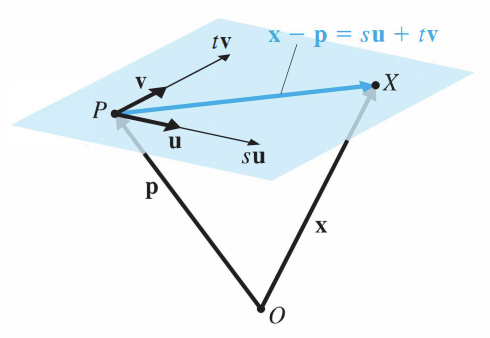
\includegraphics[scale=0.7]{VecPlane.png}
\caption{Defining a Plane with Vectors}
\label{vecplane}
\end{center}
\end{figure}
If we define the vectors as in Figure \ref{vecplane}, we can see that the distance from any general point $\vv{x}$ and $\vv{p}$ is just $\vv{x-p}$. Now notice how we can choose scalars $t$ and $s$ so that $s\vv{u} + t\vv{v} = \vv{x-p}$. Combining every possible combination of this defines the flat surface that is a plane. It follows that:
\begin{gather*}
    \vv{x} = \vv{p} + s\vv{u} + t\vv{v}
\end{gather*}
Looking at the figure, it makes sense why a single plane can't be defined with parallel direction vectors, since more than one plane could fit those conditions. Also note that plane is a 2 dimensional object, and requires two parameters to fully define it. For example, the parametric equation for $y$:
\begin{gather*}
    y = \vv{x_y} = \vv{p_y} + s\vv{u_y} + t\vv{v_y}
\end{gather*}
Since there are infinitely many lines in a plane, a line cannot be defined this way either. However, with two nonparallel normal vectors and a point, a line can defined as the set of points through $P$ perpendicular to $\vv{n}_1 $ and $\vv{n}_2$. Imagine a line being the $z$-axis, defined by two normal vectors off the $x$ and $y$ axis, with the point being the origin. Each normal vector can define it's own plane, so:
\begin{gather*}
    a_1x + b_1y + c_1z = d_1\\
    a_2x + b_2y + c_2z = d_2
\end{gather*}
The set of all $x,y,z$ that satisfy these two equations forms a line. Geometrically, this shows that the intersection of two planes forms a line.

Notice that a single equation of this type defines a different object as you increase dimensions. In $\mathbb{R}_2$, it defined a line. In $\mathbb{R}_3$, a plane, and in $R_n$, an $n-1$ dimension object called a \textit{hyperplane}. The relation between the dimension of an object $D_o$, the number of general equations required $E_o$, and the dimension of the space($D_s$) it is in:
\begin{gather*}
    D_o + E_o = D_s
\end{gather*}
This explains why the hyperplane defined by one equation is always one dimension lower than the space. It also explains why a line needs only one equation in $\mathbb{R}_2$ but two in $\mathbb{R}_3$.
\section{Systems of Linear Equations}
\subsection{Systems of Linear Equations}
A \textbf{linear equation} of $n$ variables $x_1,x_2...x_n$ is an equation that can be rewritten in the form:
\begin{gather*}
    a_1x_1 + a_2x_2 + ... a_nx_n = b
\end{gather*}
where all \textbf{coefficients} $a$ are and the \textbf{constant term} $b$ are constants. Note how the variable coefficients are all constants and not functions of $x$ or any other variable.

A \textbf{solution} of a linear equation is a vector $\ve{s_1,s_2...s_n}$ whose components satisfy the equation when the substitution $s_1 \implies x_1, s_2 \implies x_2...s_n \implies x_n$ is made.

A \textbf{system of linear equations} is a finite set of linear equations in the same variables, and its solution is a vector that is a solution to all equations in the system. The \textbf{solution set} of a system is the set of all vector solutions to that system.

A system is \textbf{consistent} if it has at least one solution and \textbf{inconsistent} if not. There are only three possibilities with linear systems, because they are lines geometrically and the line intersects are solutions.
\begin{enumerate}
    \item A single unique solution(consistent)
    \begin{itemize}
        \item Two non-parallel lines that intersect.
    \end{itemize}
    \item Infinitely many solutions(consistent)
    \begin{itemize}
        \item Two non-parallel lines that coincide(share all points).
    \end{itemize}
    \item No Solutions at all
    \begin{itemize}
        \item Two parallel lines that never intersect.
    \end{itemize}
\end{enumerate}
Two linear systems are \textbf{equivalent} if they have the same solutions(this makes sense because they can effectively be merged). One useful approach to solve is to transform equations in the system into equivalent ones that are easier to deal with.

Sometimes it is easier to solve systems by writing their coefficients into a matrix, since all their variables are the same(between equations). This matrix is called the \textbf{augmented matrix} of the system. For example:
\begin{gather*}
    x - y - z = 2\\
    3x - 3y + 2z = 16\\
    2x - y + z = 9\\
    \begin{bmatrix}
    \begin{array}{ccc|c}
    1 & -1 & -1 &2 \\
    3 & -3 & 2 & 16\\
    2 & -1 & 1 & 9
    \end{array}
    \end{bmatrix}
\end{gather*}
\subsection{Direct Methods to Solve Linear Systems}
\subsubsection{Echelon Form}
In a matrix if a variable is not present in the equation, that position is shown by $0$, for $0x$. Denoting a linear matrix by $A$ and a column vector $\vv{b}$ of constant terms of the system, the augmented matrix can be written as $[A|\vv{b}]$. A general method for solving matrices involves reducing the matrix to an \textbf{echelon form}, a sort of staircase form where the last row will hold the key to solving the entire thing.

A matrix is in \textbf{echelon form} if:
\begin{enumerate}
    \item Any all-zero rows are at the bottom
    \item In each nonzero row, the first nonzero item(the \textbf{leading entry}) is in the column to the left of any leading entries below.
\end{enumerate}
These conditions guarantee that the leading entries will form a staircase or triangle pattern, such that any column contains one or less leading entries. Once a matrix is in echelon form, it is very easy to solve and establish the number of solutions of the system.
\subsubsection{Elementary Row Operations}
Just like algebraic operations reduce an equation to equivalent equations until the variable is isolated, \textbf{elementary row operations} are operations that can transform a matrix to an equivalent \textit{reduced} matrix that is easier to work with.

These elementary row operations result in an equivalent matrix:
\begin{enumerate}
    \item Switch two rows(switch their position)
    \item Multiple any row by a nonzero constant(division implied too)
    \item Add a multiple of one row to another row(subtraction implied too)
\end{enumerate}
The process of solving a matrix by applying these operations to bring it into echelon form is called \textbf{reduction}.

Normally, you work from left to right and top down to choose a leading entry as a \textbf{pivot} and zero out(by multiplying and eliminating) the lower columns. Switching rows can make this easier. Most of the time it is easier to make the leading entry $1$. The interesting thing is that reducing a matrix into echelon form is not unique, there are many different valid echelon forms.

Elementary row operations are \textit{reversible}, such that they can be undone in the opposite direction. Rows can be switched back, added multiples can be subtracted and multiplied rows can be divided out. This leads to:

Two matrices $A$ and $B$ are equivalent if and only if there exist a sequence of elementary row operations that converts $A$ to $B$, which implies that if $A$ and $B$ can be reduced to the same echelon form then they are equivalent.

\subsubsection{Gaussian Elimination}
This entire process of reducing and solving a matrix is called \textbf{Gaussian Elimination}(though he didn't come up with it).
\begin{enumerate}
    \item Write the augmented matrix for the system
    \item Use elementary row operations to reduce into echelon form
    \item Use back substitution to solve the system
\end{enumerate}
Note that step 2 can be performed in many ways. Sometimes when solving systems this way there are more variables than equations(rows) in echelon form, which means there are infinitely many solutions. This is because the \textbf{free variables} can vary and still satisfy the equations(think of the equations as \textit{constraints} to the solution set). The non-free variables are called the \textbf{leading variables} which are the variables in the leading spot in the matrix rows.

When dealing with infinitely many solutions, they still need to be defined. If $w$ and $y$ are the leading variables and $x$ and $z$ are free, the solution set(a vector) can be written by making the substitution $x = s$ and $z = t$.
\begin{gather*}
    \begin{bmatrix}
    w\\
    x\\
    y\\
    z
    \end{bmatrix}
     = \begin{bmatrix}
     w(s)\textrm{ or }w(t)\\
     s\\
     y(s)\textrm{ or }y(t)\\
     t
     \end{bmatrix}
\end{gather*}
Since the number of leading variables is just the same as the number of nonzero rows, the number of free variables(also parameters $s$ and $t$) can be predicted before actually solving. The number of nonzero rows in an echelon form of a matrix is the same(proved later). This number is called the \textbf{rank} of the matrix. This implies that in an linear consistent system $A$ of $n$ variables:
\begin{gather*}
    \textrm{num of free variables = } n - \textrm{rank of $A$}
\end{gather*}
\subsubsection{Gauss-Jordan Elimination}
A matrix is in \textbf{reduced echelon form} if:
\begin{enumerate}
    \item It is in row echelon form
    \item The leading entry in echelon row is a $1$
    \item Each column containing a leading $1$ has zeros in all other rows
\end{enumerate}
It is not really apparent but the reduced echelon form of a matrix is unique to equivalent matrices. So every equivalent matrix has the exact same reduced form(not proved here). Many problems in geometry can be solved using a linear system.

\subsubsection{Homogeneous Systems}
There is one type of system that always has at least one solution, the \textbf{homogeneous system} where the constant term vector is always $\vv{b} = \ve{0,0,0...0}$. This means that there will always be at least one solution, where every variable is 0. It will either have the one zero solution or infinitely many solutions(a property of lines).

If there are more variables than equations in a homogeneous system then the system has an infinite number of solutions.
\begin{proof}
Since the system has one solution at least, rank($A) \leqslant m$, where $m$ is the number of equations, which is true because the number of equations is less than the number of variables. So,
\begin{gather*}
    \textrm{num of free variables} = n - \textrm{rank}(A) \geqslant n - m > 0
\end{gather*}
This shows that there is at least one free variable and there are infinite solutions.
\end{proof}
\subsubsection{Linear Systems on $\mathbb{Z}_p$}
When $p$ is a prime number, we can solve system using elimination on $\mathbb{Z}_p$. For example $x + y + z = 1$ has exactly four solutions when $p = 2$. There are three cases when one variables is $1$ and all the others are $0$. The last case arises when all variables are $1$ since $1 + 1 + 1 = 1$. You don't need to use trial and error, since elimination works on these fields just as well as in $\mathbb{R}$.
\subsection{Spanning Sets and Linear Independence}
One question: How do you find if a given vector is a linear combination of some other vectors?(see 1.1 for linear combination)

For example, imagine these three vectors:
\begin{gather*}
    \vv{a} =
    \begin{bmatrix}
        a_x\\
        a_y\\
        a_z
    \end{bmatrix}\hspace{30pt}
    \vv{b} =
    \begin{bmatrix}
        b_x\\
        b_y\\
        b_z
    \end{bmatrix}\hspace{30pt}
    \vv{d} =
    \begin{bmatrix}
        d_x\\
        d_y\\
        d_z
    \end{bmatrix}
\end{gather*}
We want to find out if $\vv{a}$ is a linear combination of $\vv{b}$ and $\vv{d}$, which means:
\begin{gather*}
    \begin{bmatrix}
        a_x\\
        a_y\\
        a_z
    \end{bmatrix}
    = c_1
    \begin{bmatrix}
        b_x\\
        b_y\\
        b_z
    \end{bmatrix}
    + c_2
    \begin{bmatrix}
        d_x\\
        d_y\\
        d_z
    \end{bmatrix}
\end{gather*}
for scalars $c_1,c_2$. This is easy though, by constructing a system of equations and using elimination on the matrix where $c_1,c_2$ are actually the \textit{variables} being solved for. If there are no solutions, then $\vv{a}$ is not a linear combination of the other two.

So, a system of linear equations $[A|\vv{b}]$ is consistent if and only if $\vv{v}$ is a linear combination of the vectors formed on the columns of $A$.

That should make sense, as it is saying there must be some values that satisfy the system, which is exactly what a consistent system is!
\subsubsection{Spanning Sets}
If $S = \{\vv{v_1},\vv{v_2}...\vv{v_k}\}$ is a set of vectors in $\mathbb{R}^n$, then the set of all the possible linear combinations of the vectors in $S$ is called the \textbf{span} of $S$. If span$(S) = \mathbb{R}^n$, then $S$ is a \textbf{spanning set} of $\mathbb{R}^n$.

Because you can multiply an extra vector by the scalar $0$, any set that \textit{contains} a spanning set is also a spanning set. An easy spanning set is the unit vectors, since they can combine in varying amounts to produce a space.
\subsubsection{Linear Independence}
This is important because we can define \textbf{linear dependence} as when a vector is a linear combination of some other vectors. For example, $\vv{v}$ is dependent on $\vv{a}$ and $\vv{b}$:
\begin{gather*}
    \vv{v} = c_1\vv{a} + c_2\vv{b}
\end{gather*}
for scalars $c_1$ and $c_2$.
However, in order for a \textit{set} of vectors to be linearly dependent, we have to define it differently, since which vector would be dependent on the rest?

A set $S$ of vectors is \textbf{linearly dependent} if there are some scalars $c$ at least one of which is nonzero such that
\begin{gather*}
    c_1\vv{v_1} + c_2\vv{v_2} + c_k\vv{v_k} = 0
\end{gather*}
If $S$ does not meet these conditions then it is \textbf{linearly independent}.

If all the scalars $c$ were $0$, then all vectors would be dependent. What linear dependence is saying is that the \textit{nontrivial} linear combination must be $0$, and so linear independence means the only way they can make $0$ is if all $c_i = 0$.

This leads to some interesting observations. For example, every vector set containing the zero vector is dependent, because the nonzero scalar could be on the zero vector with all other scalars zero, which would result in a zero(dependent) result.

The only way two vectors can be linearly dependent is if one is a multiple of the other. Why? Assume they are dependent:
\begin{gather*}
    c_1\vv{v} + c_2\vv{w} = 0\\
    \vv{v} = -\dfrac{c_2}{c_1}\vv{w}
\end{gather*}
Another way to check for linear dependence(and to find a dependence relation) is to use a system of equations, with the scalars as variables. If the vectors are columns, then the constant vector is $\vv{b} = 0$, and if there is at least one \textit{nontrivial} solution, then the set of vectors is linearly dependent.

Another method is to treat the vectors as rows of a matrix. Since performing elementary row operations results in an equivalent system, if any operation results in a new zero row, then the set is dependent. This is true because elementary row operations involve multiplying scalars and adding rows together, which is the same as a linear combination(any unused row vectors in the operation can have $c = 0$).

In other words, if the \textit{rank} of the matrix is less than the original number of equations, then the set is dependent.

One really thoughtful method concludes that if there are $m$ vectors in the set in $\mathbb{R}^n$, the set is linearly dependent if $m > n$. This is true because if the matrix form $[A,0]$ has a nontrivial solution, then we have dependence. This will always be true if we have more columns than rows(more variables(vectors) than equations), since the scalar on the "free" variable can balance out the sum of the other ones to make zero. We can always pick a scalar that works here, and so this means that if $m$(variables/num of vectors) is greater than $n$(equations/dimensions of the vector), the set is linearly dependent.
\section{Matrices}
\subsection{Matrices and Matrix Operations}
A \textbf{matrix} is a rectangular array of numbers called \textbf{entries}. A matrix is normally called $m \times n$ if it has $m$ rows and $n$ columns. Any matrix with a single row($1 \times n$) is a row matrix and single column is a column matrix. Double subscript notation(used also with 2D arrays in CS) is used to find a specific matrix element. $A_{23}$ is used to locate the element on the second row and third column of matrix $A$.

The \textbf{diagonal entries} of $A$ can be written as $A_{11}, A_{22},A_{33}...$. If $m = n$ for a matrix the matrix is a \textbf{square matrix}. A square matrix whose entries are nonzero only on the diagonal is called a \textbf{diagonal matrix} and if all those diagonal numbers are the same it's a \textbf{scalar matrix}. Finally, if all those scalars are $1$ then you have an \textbf{identity matrix}.

Two matrices are \textbf{equal} if they have the same size($m$ and $n$), and if their corresponding entries are the same. Note that even if their entries are the same but they have different sizes, they are \textit{not equal}. Even a row matrix and a column matrix with the same numbers are \textit{not equal}.
\subsubsection{Matrix Addition}
The sum of matrices(from vector addition) is just the sum of the corresponding components of the matrices. Note that this means that addition cannot be defined for matrices of different sizes.
\begin{gather*}
    A+B = [A_{ij} + B_{ij}]
\end{gather*}
Also from vectors, a scalar multiplication is carried out by multiplying the entries in the matrix as well. The \textbf{zero matrix} $O$ is a matrix of any size that is filled with just zeroes. It follows that:
\begin{gather*}
    A + O = A\qquad A - A = O
\end{gather*}
\subsubsection{Matrix Multiplication}
Multiplying matrices is a little bit more complicated. This time it's not componentwise, but more of a dot product-type setup. Start from the top left($1,1$) and then multiply each item in the row of $A$ by the corresponding entry but in the \textit{column} of $B$.
\begin{gather*}
    AB = C \implies c_{ij} = a_{i1}b_{1j} + a_{i2}b_{2j}+...
\end{gather*}
This requires that number of columns in $A$ be equal to the number of rows in $B$, and that the final matrix is going to have the number of rows in $A$ and the number of columns in $B$. This form of approaching matrix products has a lot more applications than componentwise.

Interestingly, any linear system can be written in the form of a matrix multiplication of $A\vv{x} = \vv{b}$. For example, the linear system:
\begin{gather*}
    x_1 - 2x_2 + 3x_3 = 5\\
    -x_1 + 3x_2 + x_3 = 1\\
    2x_1 - x_2 + 4x_3 = 14
\end{gather*}
can be written as:
\begin{gather*}
    \begin{bmatrix}
        1 & -2 & 3\\
        -1 & 3 & 1\\
        2 & -1 & 4\\
    \end{bmatrix}
    \begin{bmatrix}
        x_1 \\ x_2 \\ x_3
    \end{bmatrix} =
    \begin{bmatrix}
        5 \\ 1 \\ 14
    \end{bmatrix}
\end{gather*}
In fact, \textit{all} linear systems can be written this way. Of course, the system only has a solution if $\vv{b}$ is a linear combination of the columns of $A$.

An interesting consequence arises when you start to multiply matrices and unit vectors. If you multiply a unit vector by a matrix, then you'll get that row of the matrix. If you multiply in the opposite order you'll get the column of the matrix.
\begin{proof}
Let's prove that $A\hat{q}$ will give the $q$th column of $A$:
\begin{gather*}
    A\hat{q} = 0\vv{a}_1 + 0\vv{a}_2... + 1\vv{a}_q..+0\vv{a}_{q+1} = \vv{a}_q
\end{gather*}
\end{proof}
\subsubsection{Partitioned Matrices}
Sometimes it's more convenient to introduce horizontal and vertical lines into a matrix in order to divide it into matrix \textbf{blocks}. Such a matrix is called a \textbf{partitioned matrix}. There is normally a natural way to do it, as you can spot scalar, identity, diagonal, etc. submatrices inside the larger one. You can treat each submatrix as an entry in the larger matrix, which allows for multiplication and operations.

For example, some natural matrix partitions include \textbf{row-column} representations, where you partition $A$ into $A$ into rows and $B$ into columns. Also there is the \textbf{column-row} representation:
\begin{gather*}
    A = \begin{bmatrix}
        \vv{a_1} & \vv{a_2} & \vv{a_3}
    \end{bmatrix}\quad
    \textrm{as well as:}\quad B = \begin{bmatrix}
        \vv{b_1} \\ \vv{b_2} \\ \vv{b_3}
    \end{bmatrix}
\end{gather*}
Multiplying these yields $AB = \vv{a_1}\vv{b_1} + \vv{a_2}\vv{b_2}...$ which resembles a dot product expansion, this is called an \textbf{outer-product expansion}.
\subsubsection{Matrix Powers}
When $A$ and $B$ are both square matrices of the same size, you can say that $AB$ will also be $n \times n$. When $A = B$, you can define $A^2 = AA$, and $A^k = AAA...A_k$. Also, $A^1 = A$ and $A^0 = I_n$, where $I$ is the identity matrix. Similar exponent rules apply here(power and addition of exponents).
\subsubsection{The Transpose of a Matrix}
The \textbf{transpose} of an $m \times n$ matrix $A$ is the $n \times m$ matrix $A^T$ which is found just be interchanging the rows and columns of $A$.

For example, the matrix $A$:
\begin{gather*}
    A = \begin{bmatrix}
        1 & 3 & 4\\
        2 & 5 & 8
    \end{bmatrix},
    A^T = \begin{bmatrix}
        1 & 2\\
        3 & 5\\
        4 & 8
    \end{bmatrix}
\end{gather*}
In other words $A_{ij} = A^T_{ji}$.

Using this, a square matrix is \textbf{symmetric} if $A = A^T$, if you can transpose the square matrix and leave it unchanged, then the matrix is symmetric. This can be seen if the matrix entries are symmetric around the matrix's diagonal.
\subsection{Matrix Algebra}
All of the properties for the addition and scalar multiplication of vectors also carry over to matrices, including commutativity, associativity, identity, and distributivity.

If we have a set of matrices $A_1,A_2...A_k$ and a set of scalars $c_1,c_2...c_k$, then their \textbf{linear combination} is:
\begin{gather*}
    c_1A_1 + c_2A_2 + c_3A_3...c_kA_k
\end{gather*}
So the \textbf{span} of a set of matrices is the set of all linear combinations of those matrices. Therefore a set of matrices is \textbf{linearly independent} if the only solution to the above is the trivial one.
\subsubsection{Matrix Multiplication}
Matrix multiplication is a little different than real number multiplication. Here associativity holds, and also distributivity is going to hold on the left and right sides(matrix multiplication is not commutative). The identity property is also fine:
\begin{gather*}
    I_mA = A = AI_n
\end{gather*}
for a matrix $A$ with size $m \times n$. To prove these properties, partition the left matrix into rows and the right one into columns and multiply.
\subsubsection{Matrix Transpose}
Transpose properties:
\begin{gather*}
    (A^T)^T = A\qquad(A+B)^T = A^T + B^T\\
    (kA)^T = k(A^T)\qquad (AB)^T = B^TA^T\\
    (A^r)^T = (A^T)^r\textrm{ for all } r \geqslant 0
\end{gather*}
The reason the fourth property exists is because the transposed matrix will have opposite dimensions as the original. So the multiplication needs to be done in reverse for them to have the same size. This is why it's $B^TA^T$ and not the other way around.

\subsection{The Inverse of a Matrix}
Going back to the general equation of a linear system: $A\vv{x} = \vv{b}$, we can see that the solution would require a division. For example, the normal equation $ax = b$ can be solved to $x = \frac{b}{a}$ for $a \neq 0$. However, it isn't that easy for matrices. In fact, we need to find a matrix $A'$ such that $AA'$ and $A'A$ are both equal to $I$(the identity matrix, the $1$ of matrix algebra). Of course, for both products to be defined, both matrices must be square in the same dimensions. For example:
\begin{gather*}
    A = \begin{bmatrix}
        2 & 5 \\ 1 & 3
    \end{bmatrix}
    \quad A' = \begin{bmatrix}
        3 & -5 \\ -1 & 2
    \end{bmatrix}
\end{gather*}
Multiply these two in any order will yield $I_2$. Interesting consequence here: the zero matrix in any dimensions doesn't have an inverse, because you can't have $OO' = 1$.

Now this begs the question, can a matrix have multiple inverses? The answer there is no and we can prove it by showing that any general matrices that satisfy the inverse definition are actually the same matrix.
\begin{proof}
\begin{gather*}
    AA' = I = A'A\qquad AA'' = I = A''A\\
    A' = A'I = A'(AA'') = (A'A)A'' = IA'' = A''
\end{gather*}
The above used associativity of multiplication in matrices and the identity property. This shows that any inverses are actually the same inverse.
\end{proof}
The actual notation for this inverse is $A^{-1}$, which should make sense as an inverse. Note that you \textbf{cannot divide by a matrix}, so $A^{-1} \neq \frac{1}{A}$, if you need to divide by a matrix just multiply by it's inverse.

So now we can use matrix inverses in order to solve our original problem. It turns out that if $A$ is invertible and square, then the system $A\vv{x} = \vv{b}$ has a unique solution given by $\vv{x} = A^{-1}\vv{b}$ for any $\vv{b}$ in $\mathbb{R}^n$.
\begin{proof}
\begin{gather*}
    A\vv{x} \Rightarrow A(A^{-1}\vv{b}) \Rightarrow (AA^{-1})\vv{b} \Rightarrow I\vv{b} = \vv{b}
\end{gather*}
To prove this is a unique solution just try this with another vector $\vv{y}$ in place of $\vv{x}$, and multiply both sides of $A\vv{y} = \vv{b}$ by $A^{-1}$ and you'll end up with the same solution. Therefore it must be unique.
\end{proof}
So to actually find the inverse of a matrix, it's a little more complicated. For a $2 \times 2$ matrix, we can derive a pretty simple formula:
\begin{gather*}
    A^{-1} = \frac{1}{ad - bc}\begin{bmatrix}
        d & -b \\ -c & a
    \end{bmatrix} = \frac{1}{\det A}\begin{bmatrix}
        d & -b \\ -c & a
    \end{bmatrix}
\end{gather*}
Where $ad - bc$ is the \textbf{determinant} of $A$. Therefore, the inverse exists if and only if the determinant isn't zero. So the inverse is possible when $ad - bc \neq 0$. Later we will see how a determinant can be defined for all square matrices.
\begin{proof}
\begin{gather*}
\begin{bmatrix}
    a & b \\ c & d
\end{bmatrix}
\begin{bmatrix}
    d  & -b \\ -c & a
\end{bmatrix} =
\begin{bmatrix}
    ad - bc & -ab + ba \\ cd - dc & -cb + da
\end{bmatrix} =
\begin{bmatrix}
    ad - bc & 0 \\ 0 & ad - bc
\end{bmatrix} =
\det A
\begin{bmatrix}
    1 & 0 \\ 0 & 1
\end{bmatrix}
\end{gather*}
Now take the starting step and the formed identity matrix and multiply both sides by $\frac{1}{\det A}$, which will show you how you can get $AA^{-1} = I$. If you try it with $\det A = 0$, you'll see that the second row of the matrix would just become a multiple of the first one.
\end{proof}
It might seem like inversion is an easier method to solve systems now, but elimination works for more matrices and is almost always faster than inversion.

\subsubsection{Properties of Invertible Matrices}
\begin{enumerate}
    \item $(A^{-1})^{-1} = A$
    \item $(cA)^{-1} = \frac{1}{c}A^{-1}$
    \item $(AB)^{-1} = B^{-1}A^{-1}$
    \item $(A^T)^{-1} = (A^{-1})^T$
    \item $(A^n)^{-1} = (A^{-1})^n$ for all nonnegative $n$
\end{enumerate}
We can also define negative exponents:
\begin{gather*}
    A^{-n} = (A^{-1})^n = (A^n)^{-1}
\end{gather*}
\subsubsection{Elementary Matrices}
An \textbf{elementary matrix} is any matrix that can be obtained by performing an elementary row operation on an identity matrix. There are three elementary row operations, so there are three types of elementary matrices. This means that performing an elementary row operation is the same as multiplying by an identity matrix that has that operation performed on it. So since elementary row operations can be reversed, it makes sense that these matrices are invertible. Also, any inverted elementary matrix is also an elementary matrix.

This all leads to the \textbf{Fundamental Theorem of Invertible Matrices} whcih is a set of 5 statements which are all \textbf{equivalent}, meaning that they're either all true or all false.
\begin{enumerate}
    \item $A$ is invertible
    \item $A\vv{x} = \vv{b}$ has one unique solution for every $\vv{b}$
    \item $A\vv{x} = \vv{0}$ has only the trivial solution
    \item The reduced row echelon form of $A$ is $I_n$
    \item $A$ is a product of elementary matrices
\end{enumerate}
\begin{proof}
We can prove this by showing that each statement proves the next, so that they are either all true or all false together. Each point will show that if the current point is true, the next one must also be true.
\begin{descenum}
    \item We already showed this earlier.
    \item If we choose $\vv{0}$ as our $\vv{b}$, it only has one solution which means that solution must be the trivial one.
    \item Because the solution will have $x_1,x_2,x_3...=0$, we know that the row reduced form(since it's unique) will be the identity matrix. Think about how you get the solutions from the row reduced form, and think of that in reverse.
    \item Because the row reduced form is the identity matrix(and all elementary row operations are reversible), we can see that by multiplying $I_n$ by some elementary matrices, we get $A$.
    \item Because $A$ is a product of elementary matrices, and all elementary matrices are invertible, we can say that $A$ is also invertible.
\end{descenum}
\end{proof}
If $A$ and $B$ is are square matrices such that either $AB = I$ or $BA = I$, then $A$ is invertible and $B = A^{-1}$.
\begin{proof}
Suppose $BA = I$, then if we think about $A\vv{x} = \vv{0}$, and multiply both sides on the left by $B \Rightarrow BA\vv{x} = B\vv{0} \Rightarrow I\vv{x} = 0$. So because $A\vv{x} = \vv{0}$ only has the trivial solution, $A$ is invertible by $(3)$. If you use $BA = I \Rightarrow BAA^{-1} = A^{-1} \Rightarrow B = A^{-1}$
\end{proof}
Let $A$ be a square matrix, if a sequence of elementary row operations converts $A \Rightarrow I$, then the same sequence applied to $I$ will convert it to $A^{-1}$.
\begin{proof}
This proof is quite simple, just call the sequence of elementary matrices $B$, which gives $BA = I$. As a consequence of the previous theorem, $BI = B = A^{-1}$.
\end{proof}
\subsubsection{The Gauss-Jordan Method}
We can perform row operations on two matrices at the same time by just adjoining them into what's called a "super-augmented matrix" $[A | I]$, which is a combination of $A$ and the identity matrix. Because of the previous theorem, if we row reduce $A$(but apply those operations to the whole matrix, we will end up with $[I | A^{-1}]$. You can also think of this as solving a bunch of linear systems. Since $I = \vv{e}_1, \vv{e}_2...$, you can denote each column of $A$ by $\vv{x}_1, \vv{x}_2...$ which gives you the linear systems:
\begin{gather*}
    A\vv{x}_1 = \vv{e}_1, A\vv{x}_2 = \vv{e}_2...\Rightarrow [A|I_n]
\end{gather*}
\subsection{The LU Factorization}
The LU method is a method of \textit{matrix factorization}, where $U$ is the row reduction of $A$ (not reduced though), and using the elementary matrices we can write:
\begin{gather*}
    E_nE_{n-1}E_{n-2}...E_1A = U
\end{gather*}
Solving for $A$, we get $A = LU$, where $L = E_1^{-1}E_2^{-1}...$ where $U$ is \textbf{upper triangular} and $L$ is \textbf{lower triangular}. Note that because no row reductions were necessary. $A$ has an $LU$ factorization, because all the elementary matrices were lower triangular, and inverses and products of lower triangular matrices are lower triangular.

We can use this so solve $A\vv{x} = \vv{b}$, because if $A = LU$, then $L(U\vv{x}) = \vv{b}$, and we can set $\vv{y} = U\vv{x}$, and solve $L\vv{y} = \vv{b}$ by normal substitution (this is because of the triangular shape of the matrix). Then you can solve $U\vv{x} = \vv{y}$ using the reverse order substitution (back substitution). If we reduce a matrix $A$ without interchanging rows, we can use $R_i - kR_j$ to do all elementary operations, in which case $k$ will be the element $(i,j)$ in $L$. Notice the $-$ sign in the expression.

When doing this, it's important to perform elementary row operations from top to bottom in each column, so that you can use the above property of the multiplier $k$.

An even \textit{faster} way to find $L$ is to use the pivots in each column and construct one column matrices with all the elements on or below the pivot, but normalize them by the pivot. This will give you a lower triangular matrix with the unfilled spaces $0$.

If $A$ is invertible with an $LU$ factorization, then $L$ and $U$ are unique.

\begin{proof}
We can prove uniqueness by proving $A = LU$ and the other $A = L_1U_1$ are indeed the same the matrices. All $L$ are lower triangular and all $U$ are upper triangular. So we know from $A$ that $LU = L_1U_1$ So if we start with:
\begin{gather*}
    L_1^{-1}(LU)U^{-1} = L_1^{-1}(L_1U_1)U^{-1} \implies L_1^{-1}L I = U_1U^{-1}
\end{gather*}
Because all $L$ are lower triangular and all $U$ are upper triangular, the left side is lower and the right side is upper. The only matrix where this works is the identity matrix, which gives $L = L_1$ and $U = U_1$.
\end{proof}
Now we can focus on the case where row switching is actually necessary to reduce (e.g. when the top row has a 0 in the first entry). The elementary matri(ces) corresponding to the needed switching operations can be multiplied into a \textbf{permutation matrix} $P$, and the rest are $E$, such that $EPA = U$, so $A = P^{-1}E^{-1}U = P^{-1}LU$, since $E^{-1} = L$.

If $P$ is a permutation matrix, then $P^{-1} = P^T$.
\begin{proof}
We need to prove that $PP^T = I$, but any row of $P$ is just a column of $P^T$, which are both the same unit vector. Since matrix multiplication is the same as multiplying the rows of the first vector by the columns of the second is just dot product of the same unit vector, or $1$. Multiplying the wrong unit vectors together gives $0$, which gives the final identity matrix.
\end{proof}
\end{document}
